\documentclass[12pt,]{article}
\usepackage{lmodern}
\usepackage{amssymb,amsmath}
\usepackage{ifxetex,ifluatex}
\usepackage{fixltx2e} % provides \textsubscript
\ifnum 0\ifxetex 1\fi\ifluatex 1\fi=0 % if pdftex
  \usepackage[T1]{fontenc}
  \usepackage[utf8]{inputenc}
\else % if luatex or xelatex
  \ifxetex
    \usepackage{mathspec}
  \else
    \usepackage{fontspec}
  \fi
  \defaultfontfeatures{Ligatures=TeX,Scale=MatchLowercase}
    \setmainfont[]{Times New Roman}
\fi
% use upquote if available, for straight quotes in verbatim environments
\IfFileExists{upquote.sty}{\usepackage{upquote}}{}
% use microtype if available
\IfFileExists{microtype.sty}{%
\usepackage{microtype}
\UseMicrotypeSet[protrusion]{basicmath} % disable protrusion for tt fonts
}{}
\usepackage[margin=2.54cm]{geometry}
\usepackage{hyperref}
\hypersetup{unicode=true,
            pdftitle={The Effect of Water Quality Parameters on Dissolved Oxygen Concentrations in Oahu},
            pdfauthor={Gaby Garcia},
            pdfborder={0 0 0},
            breaklinks=true}
\urlstyle{same}  % don't use monospace font for urls
\usepackage{color}
\usepackage{fancyvrb}
\newcommand{\VerbBar}{|}
\newcommand{\VERB}{\Verb[commandchars=\\\{\}]}
\DefineVerbatimEnvironment{Highlighting}{Verbatim}{commandchars=\\\{\}}
% Add ',fontsize=\small' for more characters per line
\usepackage{framed}
\definecolor{shadecolor}{RGB}{248,248,248}
\newenvironment{Shaded}{\begin{snugshade}}{\end{snugshade}}
\newcommand{\KeywordTok}[1]{\textcolor[rgb]{0.13,0.29,0.53}{\textbf{#1}}}
\newcommand{\DataTypeTok}[1]{\textcolor[rgb]{0.13,0.29,0.53}{#1}}
\newcommand{\DecValTok}[1]{\textcolor[rgb]{0.00,0.00,0.81}{#1}}
\newcommand{\BaseNTok}[1]{\textcolor[rgb]{0.00,0.00,0.81}{#1}}
\newcommand{\FloatTok}[1]{\textcolor[rgb]{0.00,0.00,0.81}{#1}}
\newcommand{\ConstantTok}[1]{\textcolor[rgb]{0.00,0.00,0.00}{#1}}
\newcommand{\CharTok}[1]{\textcolor[rgb]{0.31,0.60,0.02}{#1}}
\newcommand{\SpecialCharTok}[1]{\textcolor[rgb]{0.00,0.00,0.00}{#1}}
\newcommand{\StringTok}[1]{\textcolor[rgb]{0.31,0.60,0.02}{#1}}
\newcommand{\VerbatimStringTok}[1]{\textcolor[rgb]{0.31,0.60,0.02}{#1}}
\newcommand{\SpecialStringTok}[1]{\textcolor[rgb]{0.31,0.60,0.02}{#1}}
\newcommand{\ImportTok}[1]{#1}
\newcommand{\CommentTok}[1]{\textcolor[rgb]{0.56,0.35,0.01}{\textit{#1}}}
\newcommand{\DocumentationTok}[1]{\textcolor[rgb]{0.56,0.35,0.01}{\textbf{\textit{#1}}}}
\newcommand{\AnnotationTok}[1]{\textcolor[rgb]{0.56,0.35,0.01}{\textbf{\textit{#1}}}}
\newcommand{\CommentVarTok}[1]{\textcolor[rgb]{0.56,0.35,0.01}{\textbf{\textit{#1}}}}
\newcommand{\OtherTok}[1]{\textcolor[rgb]{0.56,0.35,0.01}{#1}}
\newcommand{\FunctionTok}[1]{\textcolor[rgb]{0.00,0.00,0.00}{#1}}
\newcommand{\VariableTok}[1]{\textcolor[rgb]{0.00,0.00,0.00}{#1}}
\newcommand{\ControlFlowTok}[1]{\textcolor[rgb]{0.13,0.29,0.53}{\textbf{#1}}}
\newcommand{\OperatorTok}[1]{\textcolor[rgb]{0.81,0.36,0.00}{\textbf{#1}}}
\newcommand{\BuiltInTok}[1]{#1}
\newcommand{\ExtensionTok}[1]{#1}
\newcommand{\PreprocessorTok}[1]{\textcolor[rgb]{0.56,0.35,0.01}{\textit{#1}}}
\newcommand{\AttributeTok}[1]{\textcolor[rgb]{0.77,0.63,0.00}{#1}}
\newcommand{\RegionMarkerTok}[1]{#1}
\newcommand{\InformationTok}[1]{\textcolor[rgb]{0.56,0.35,0.01}{\textbf{\textit{#1}}}}
\newcommand{\WarningTok}[1]{\textcolor[rgb]{0.56,0.35,0.01}{\textbf{\textit{#1}}}}
\newcommand{\AlertTok}[1]{\textcolor[rgb]{0.94,0.16,0.16}{#1}}
\newcommand{\ErrorTok}[1]{\textcolor[rgb]{0.64,0.00,0.00}{\textbf{#1}}}
\newcommand{\NormalTok}[1]{#1}
\usepackage{graphicx,grffile}
\makeatletter
\def\maxwidth{\ifdim\Gin@nat@width>\linewidth\linewidth\else\Gin@nat@width\fi}
\def\maxheight{\ifdim\Gin@nat@height>\textheight\textheight\else\Gin@nat@height\fi}
\makeatother
% Scale images if necessary, so that they will not overflow the page
% margins by default, and it is still possible to overwrite the defaults
% using explicit options in \includegraphics[width, height, ...]{}
\setkeys{Gin}{width=\maxwidth,height=\maxheight,keepaspectratio}
\IfFileExists{parskip.sty}{%
\usepackage{parskip}
}{% else
\setlength{\parindent}{0pt}
\setlength{\parskip}{6pt plus 2pt minus 1pt}
}
\setlength{\emergencystretch}{3em}  % prevent overfull lines
\providecommand{\tightlist}{%
  \setlength{\itemsep}{0pt}\setlength{\parskip}{0pt}}
\setcounter{secnumdepth}{5}
% Redefines (sub)paragraphs to behave more like sections
\ifx\paragraph\undefined\else
\let\oldparagraph\paragraph
\renewcommand{\paragraph}[1]{\oldparagraph{#1}\mbox{}}
\fi
\ifx\subparagraph\undefined\else
\let\oldsubparagraph\subparagraph
\renewcommand{\subparagraph}[1]{\oldsubparagraph{#1}\mbox{}}
\fi

%%% Use protect on footnotes to avoid problems with footnotes in titles
\let\rmarkdownfootnote\footnote%
\def\footnote{\protect\rmarkdownfootnote}

%%% Change title format to be more compact
\usepackage{titling}

% Create subtitle command for use in maketitle
\providecommand{\subtitle}[1]{
  \posttitle{
    \begin{center}\large#1\end{center}
    }
}

\setlength{\droptitle}{-2em}

  \title{The Effect of Water Quality Parameters on Dissolved Oxygen
Concentrations in Oahu}
    \pretitle{\vspace{\droptitle}\centering\huge}
  \posttitle{\par}
  \subtitle{\url{https://github.com/gdg12/FinalDataAnalyticsProject}}
  \author{Gaby Garcia}
    \preauthor{\centering\large\emph}
  \postauthor{\par}
    \date{}
    \predate{}\postdate{}
  

\begin{document}
\maketitle
\begin{abstract}
Water bodies with higher concentrations of dissolved oxygen tend to have
more diverse and stable aquatic ecossytems. This data analysis focuses
on the water quality parameters that have statistical significance on
dissolved oxygen concentrations at coastal monitoring locations on the
island of Oahu. A multiple linear regression was performed encompassing
all continuous water quality parameters that were not multicollineated
with dissolved oxygen. The analysis demonstrates that enterococcus,
temperature, pH, and salinity are statistically significant explanatory
variables for dissolved oxygen concentrations in Oahu. A spatial
analysis of dissolved oxygen concentrations was performed for the North,
South, East, and West coasts of Oahu; however, no trend was apparent. A
temporal analysis of dissolved oxygen was performed; dissolved oxygen
concentrations were lowest in the summer months and highest in the
winter months.
\end{abstract}

\newpage

\tableofcontents 

\section{Setup}\label{setup}

\section{Research Question and
Rationale}\label{research-question-and-rationale}

\section{Dataset Information}\label{dataset-information}

\section{Exploratory Data Analysis and
Wrangling}\label{exploratory-data-analysis-and-wrangling}

\section{Analysis}\label{analysis}

\section{Summary and Conclusions}\label{summary-and-conclusions}

\newpage

\listoftables 

\subsection{\texorpdfstring{``The Effect of Water Temperature on DO
Concentrations across
Oahu''}{The Effect of Water Temperature on DO Concentrations across Oahu}}\label{the-effect-of-water-temperature-on-do-concentrations-across-oahu}

\subsection{\texorpdfstring{``The Effect of pH on DO Concentrations
across
Oahu''}{The Effect of pH on DO Concentrations across Oahu}}\label{the-effect-of-ph-on-do-concentrations-across-oahu}

\subsection{\texorpdfstring{``The Effect of Turbidity on DO
Concentrations across
Oahu''}{The Effect of Turbidity on DO Concentrations across Oahu}}\label{the-effect-of-turbidity-on-do-concentrations-across-oahu}

\subsection{\texorpdfstring{``The Effect of Salinity on DO
Concentrations across
Oahu''}{The Effect of Salinity on DO Concentrations across Oahu}}\label{the-effect-of-salinity-on-do-concentrations-across-oahu}

\subsection{\texorpdfstring{``Correlation of Oahu Water Quality
Parameters''}{Correlation of Oahu Water Quality Parameters}}\label{correlation-of-oahu-water-quality-parameters}

\subsection{\texorpdfstring{``Effect of Region on Range of Dissolved
Oxygen Concentrations in
Oahu''}{Effect of Region on Range of Dissolved Oxygen Concentrations in Oahu}}\label{effect-of-region-on-range-of-dissolved-oxygen-concentrations-in-oahu}

\subsection{\texorpdfstring{``The Effect of Sample Date on Dissolved
Oxygen Concentrations in North
Oahu''}{The Effect of Sample Date on Dissolved Oxygen Concentrations in North Oahu}}\label{the-effect-of-sample-date-on-dissolved-oxygen-concentrations-in-north-oahu}

\subsection{\texorpdfstring{``The Effect of Sample Date on Dissolved
Oxygen Concentrations in South
Oahu''}{The Effect of Sample Date on Dissolved Oxygen Concentrations in South Oahu}}\label{the-effect-of-sample-date-on-dissolved-oxygen-concentrations-in-south-oahu}

\subsection{\texorpdfstring{``The Effect of Sample Date on Dissolved
Oxygen Concentrations in West
Oahu''}{The Effect of Sample Date on Dissolved Oxygen Concentrations in West Oahu}}\label{the-effect-of-sample-date-on-dissolved-oxygen-concentrations-in-west-oahu}

\subsection{\texorpdfstring{``The Effect of Sample Date on Dissolved
Oxygen Concentrations in East
Oahu''}{The Effect of Sample Date on Dissolved Oxygen Concentrations in East Oahu}}\label{the-effect-of-sample-date-on-dissolved-oxygen-concentrations-in-east-oahu}

\subsection{\texorpdfstring{``The Effect of Sample Date on Dissolved
Oxygen Concentrations in
Oahu''}{The Effect of Sample Date on Dissolved Oxygen Concentrations in Oahu}}\label{the-effect-of-sample-date-on-dissolved-oxygen-concentrations-in-oahu}

\subsection{\texorpdfstring{``The Effect of Sample Date on Water
Temperatures in
Oahu''}{The Effect of Sample Date on Water Temperatures in Oahu}}\label{the-effect-of-sample-date-on-water-temperatures-in-oahu}

\subsection{\texorpdfstring{``The Effect of Sample Date on pH in
Oahu''}{The Effect of Sample Date on pH in Oahu}}\label{the-effect-of-sample-date-on-ph-in-oahu}

\subsection{\texorpdfstring{``The Effect of Sample Date on Salinity in
Oahu''}{The Effect of Sample Date on Salinity in Oahu}}\label{the-effect-of-sample-date-on-salinity-in-oahu}

\newpage

\listoffigures  \newpage

tbls= \#Setup

\begin{Shaded}
\begin{Highlighting}[]
\KeywordTok{setwd}\NormalTok{(}\StringTok{"~/Desktop/Environmental Data Analytics/Environmental_Data_Analytics/Final Project/Raw Data"}\NormalTok{)}
\NormalTok{OahuData<-}\KeywordTok{read.csv}\NormalTok{(}\StringTok{'OahuData.csv'}\NormalTok{)}
\end{Highlighting}
\end{Shaded}

\subsection{Load Necessary Packages}\label{load-necessary-packages}

\begin{Shaded}
\begin{Highlighting}[]
\KeywordTok{library}\NormalTok{(tidyverse)}
\KeywordTok{library}\NormalTok{(tidyr)}
\KeywordTok{library}\NormalTok{(ggplot2)}
\KeywordTok{library}\NormalTok{(GGally)}
\KeywordTok{library}\NormalTok{(dplyr)}
\KeywordTok{library}\NormalTok{(plyr)}
\KeywordTok{library}\NormalTok{(lubridate)}
\KeywordTok{library}\NormalTok{(viridis)}
\KeywordTok{library}\NormalTok{(RColorBrewer)}
\KeywordTok{library}\NormalTok{(colormap)}
\KeywordTok{library}\NormalTok{(gridExtra)}
\KeywordTok{library}\NormalTok{(corrplot)}
\KeywordTok{library}\NormalTok{(nlme)}
\KeywordTok{library}\NormalTok{(lsmeans)}
\KeywordTok{library}\NormalTok{(multcompView)}
\KeywordTok{library}\NormalTok{(trend)}
\KeywordTok{library}\NormalTok{(mapview)}
\KeywordTok{library}\NormalTok{(leaflet)}
\KeywordTok{library}\NormalTok{(sf)}
\KeywordTok{library}\NormalTok{(car)}
\KeywordTok{library}\NormalTok{(stats)}
\KeywordTok{library}\NormalTok{(wesanderson)}
\KeywordTok{library}\NormalTok{(scales)}
\KeywordTok{library}\NormalTok{(extrafont)}
\end{Highlighting}
\end{Shaded}

\subsection{Set GGPlot Theme}\label{set-ggplot-theme}

\begin{Shaded}
\begin{Highlighting}[]
\NormalTok{gabytheme <-}\StringTok{ }\KeywordTok{theme_bw}\NormalTok{(}\DataTypeTok{base_size =} \DecValTok{14}\NormalTok{) }\OperatorTok{+}\StringTok{ }
\StringTok{  }\KeywordTok{theme}\NormalTok{(}\DataTypeTok{plot.title=}\KeywordTok{element_text}\NormalTok{(}\DataTypeTok{face=}\StringTok{"bold"}\NormalTok{, }\DataTypeTok{size=}\StringTok{"15"}\NormalTok{, }\DataTypeTok{color=}\StringTok{"Indianred4"}\NormalTok{, }\DataTypeTok{hjust=}\FloatTok{0.5}\NormalTok{),}
        \DataTypeTok{axis.title=}\KeywordTok{element_text}\NormalTok{(}\DataTypeTok{face=}\StringTok{"bold.italic"}\NormalTok{, }\DataTypeTok{size=}\DecValTok{11}\NormalTok{, }\DataTypeTok{color=}\StringTok{"black"}\NormalTok{),}
\DataTypeTok{axis.text =} \KeywordTok{element_text}\NormalTok{(}\DataTypeTok{face=}\StringTok{"bold"}\NormalTok{, }\DataTypeTok{size=}\DecValTok{10}\NormalTok{, }\DataTypeTok{color =} \StringTok{"black"}\NormalTok{), }
\DataTypeTok{panel.background=}\KeywordTok{element_rect}\NormalTok{(}\DataTypeTok{fill=}\StringTok{"white"}\NormalTok{, }\DataTypeTok{color=}\StringTok{"darkblue"}\NormalTok{), }
\DataTypeTok{panel.border =} \KeywordTok{element_rect}\NormalTok{(}\DataTypeTok{color =} \StringTok{"black"}\NormalTok{, }\DataTypeTok{size =} \DecValTok{2}\NormalTok{),}
\DataTypeTok{legend.position =} \StringTok{"top"}\NormalTok{, }\DataTypeTok{legend.background =} \KeywordTok{element_rect}\NormalTok{(}\DataTypeTok{fill=}\StringTok{"white"}\NormalTok{, }\DataTypeTok{color=}\StringTok{"black"}\NormalTok{),}
            \DataTypeTok{legend.key =} \KeywordTok{element_rect}\NormalTok{(}\DataTypeTok{fill=}\StringTok{"transparent"}\NormalTok{, }\DataTypeTok{color=}\StringTok{"NA"}\NormalTok{))}
\KeywordTok{theme_set}\NormalTok{(gabytheme)}
\end{Highlighting}
\end{Shaded}

\section{Research Question and
Rationale}\label{research-question-and-rationale-1}

The economic well being of island states such as Hawaii partially
depends on thriving coastal ecosystems. Therefore, it is important to
analyze time series water quality data featuring parameters such as
dissolved oxygen. Dissolved oxygen (DO) is one of the best indicators of
a water body's health. Water bodies with higher DO concentrations are
healthier and support diverse aquatic plants and animals. Water bodies
with low DO concentrations are often severely polluted. The amount of
dissolved oxygen that a specific water body can hold is a function of
altitude (atmospheric pressure), volume of water, amount of nutrients in
the water, aquatic organisms in the water, salinity, water temperature,
and the amount of other substances dissolved in the water, in addition
to more parameters. Cool water can hold more oxygen than warm water,
with variations ranging from seasonal to time of day or night. Water
with higher salinity has a lower DO concentration than water with lower
salinity at the same temperature. I am interested in examining what
water quality parameters affects dissolved oxygen concentrations in
Hawaii.

After some searching for water quality data on data.gov, I found a
dataset from the Monitoring Section of the State of Hawaii, Department
of Health, Clean Water Branch (CWB). The CWB collected water quality
field parameters at over 300 coastal monitoring locations in all of
Hawaii's islands using well-established instruments and methodologies.
The original dataset I found on data.gov spanned 1999-2006. Because I
wanted to account for more recent data, I found the complete dataset
spanning through 2019 on the Hawaii Clean Water Branch's website. The
complete list of relevant parameters are: Location Identifier, Location
Name, Island, Latitude of Sample, Longitude of Sample, Sample Number,
Date Sample was Collected, Time Sample was collected, Enterococci,
Temperature, Salinity, Dissolved Oxygen, Percent Saturation of Dissolved
Oxygen, pH, turbidity, Specific Heat of Water (Cp), and relevant
comments about water/weather conditions (if applicable). I decided to
filter the data for the island of Oahu only because the original dataset
included data for all of the islands, and Oahu is home to two-thirds of
Hawaii's population and hosts Honolulu, the capital. My reasoning was
that a higher island population could lead to more water body pollution.
In addition, I left out Percent Saturation of Dissolved Saturation as an
explanatory variable because

The null hypothesis of this statistical test is that pH, turbidity,
salinity, temperature, enterococcus concentrations, and specific heat
have no effect on the dissolved oxygen concentrations in Oahu. This
would be represented by the equation xYi=Bo+Ei. The alternative
hypothesis is that at least one of the predictor variables have an
effect on dissolved oxygen concentrations in Oahu, which would be
represented by the equation xYi=Bo +B1X1 +BnXn+\ldots{} +Ei. My research
questions are: 1.) Which of the parameters have a statistically
significant relationship with dissolved oxygen concentrations? Of these
relevant parameters, which of them have the most significant effect on
dissolved oxygen concentrations over time? What is the magnitude and
direction of any effects? 2. Do dissolved oxygen concentrations vary
spatially across the island of Oahu?

\newpage

\section{Dataset Information}\label{dataset-information-1}

Water Quality Data was sampled by the State of Hawaii Department of
Health Clean Water Branch (specifically, their Beach Monitoring
Program).The dataset contains data from the Statewide Water Quality
Sampling Dataset from 373 coastal monitoring sites in Hawaii from
1999-2019. All sampling and testing was done in accordance with test
procedures approved under 40 CFR Part 136 unless other test procedures
have been specified in the permit or approved by the director.

Data only from the Island of Oahu was selected from 01/01/1999 to
04/12/2019.

\subsection{Omit NA's from Data (GLM 12 lesson says to do
so)}\label{omit-nas-from-data-glm-12-lesson-says-to-do-so}

\begin{Shaded}
\begin{Highlighting}[]
\NormalTok{OahuDataClean<-}\StringTok{ }\KeywordTok{na.omit}\NormalTok{(OahuData) }
\end{Highlighting}
\end{Shaded}

\subsection{Change Date from Factor to Date
Object}\label{change-date-from-factor-to-date-object}

\begin{Shaded}
\begin{Highlighting}[]
\NormalTok{OahuDataClean}\OperatorTok{$}\NormalTok{Date<-}\KeywordTok{as.Date}\NormalTok{(OahuDataClean}\OperatorTok{$}\NormalTok{Date, }\DataTypeTok{format =} \StringTok{"%m/%d/%y"}\NormalTok{) }
\end{Highlighting}
\end{Shaded}

\subsubsection{Add a Week, Month, and Year Column to Dataframe Using
Mutate
Function}\label{add-a-week-month-and-year-column-to-dataframe-using-mutate-function}

\begin{Shaded}
\begin{Highlighting}[]
\NormalTok{OahuDataClean<-}\KeywordTok{mutate}\NormalTok{(OahuDataClean, }\DataTypeTok{Week =} \KeywordTok{week}\NormalTok{(Date))}
\NormalTok{OahuDataClean<-}\StringTok{ }\KeywordTok{mutate}\NormalTok{(OahuDataClean, }\DataTypeTok{Month =} \KeywordTok{month}\NormalTok{(Date))}
\NormalTok{OahuDataClean<-}\StringTok{ }\KeywordTok{mutate}\NormalTok{(OahuDataClean, }\DataTypeTok{Year =} \KeywordTok{year}\NormalTok{(Date))}
\end{Highlighting}
\end{Shaded}

\subsection{Create Data Structure
Table}\label{create-data-structure-table}

\begin{Shaded}
\begin{Highlighting}[]
\NormalTok{OahuDataCleanSummary<-OahuDataClean}\OperatorTok
\StringTok{  }\KeywordTok{group_by}\NormalTok{(Month)}\OperatorTok
\StringTok{ }\KeywordTok{summarize}\NormalTok{(}\DataTypeTok{MeanDO=}\KeywordTok{mean}\NormalTok{(DO, }\DataTypeTok{na.rm=}\OtherTok{TRUE}\NormalTok{), }\DataTypeTok{MeanDOPercentSaturation=}\KeywordTok{mean}\NormalTok{(DissolvedOxygenSaturation, }\DataTypeTok{na.rm=}\OtherTok{TRUE}\NormalTok{), }\DataTypeTok{MeanWaterTemperature=}\KeywordTok{mean}\NormalTok{(Temperature, }\DataTypeTok{na.rm=}\OtherTok{TRUE}\NormalTok{) , }\DataTypeTok{MeanSalinity=}\KeywordTok{mean}\NormalTok{(Salinity,}\DataTypeTok{na.rm=}\OtherTok{TRUE}\NormalTok{), }\DataTypeTok{MeanTurbidity=}\KeywordTok{mean}\NormalTok{(Turbidity,}\DataTypeTok{na.rm=}\OtherTok{TRUE}\NormalTok{), }\DataTypeTok{MeanpH=}\KeywordTok{mean}\NormalTok{(pH,}\DataTypeTok{na.rm=}\OtherTok{TRUE}\NormalTok{), }\DataTypeTok{MeanEnterococcus=}\KeywordTok{mean}\NormalTok{(Enterococcus,}\DataTypeTok{na.rm=}\OtherTok{TRUE}\NormalTok{), }\DataTypeTok{meanCP=}\KeywordTok{mean}\NormalTok{(CP.Result, }\DataTypeTok{na.rm=}\OtherTok{TRUE}\NormalTok{))}
\end{Highlighting}
\end{Shaded}

\newpage

\section{Exploratory Data Analysis and
Wrangling}\label{exploratory-data-analysis-and-wrangling-1}

They only want to see code for data exploration and wrangling, not for
data visualization Make sure to write a paragraph discussing whatI did
to wrangle my data

• Your data exploration section should contain at least five lines of
code that generate summary information about your dataset (or components
therein) • Your data exploration section should contain at least three
graphs • Your statistical modeling section should contain at least three
tests, including the rationale why you took the approach you did. Ensure
you have met assumptions of tests or that you justify moving forward
without meeting assumptions. • Your data visualization section should
contain at least three graphs.

\subsection{Structure of Water Data}\label{structure-of-water-data}

\begin{Shaded}
\begin{Highlighting}[]
\KeywordTok{str}\NormalTok{(OahuDataClean)}
\end{Highlighting}
\end{Shaded}

\begin{verbatim}
## 'data.frame':    22991 obs. of  22 variables:
##  $ LocationIdentifier       : int  177 253 263 289 265 171 249 273 233 250 ...
##  $ LocationName             : Factor w/ 166 levels "Ala Moana Lagoon",..: 134 85 150 128 135 31 101 137 114 151 ...
##  $ Island                   : Factor w/ 1 level "Oahu": 1 1 1 1 1 1 1 1 1 1 ...
##  $ LatDecDeg                : num  21.6 21.6 21.7 21.7 21.6 ...
##  $ LongDecDeg               : num  -158 -158 -158 -158 -158 ...
##  $ CP                       : Factor w/ 13 levels "","<",">","E",..: 2 1 2 2 2 2 2 2 1 2 ...
##  $ CP.Result                : num  1 1 1 1 1 1 1 1 1 1 ...
##  $ Ent                      : Factor w/ 14 levels "","<","<\xca",..: 1 1 1 1 1 1 1 1 1 1 ...
##  $ Enterococcus             : num  10 2.3 10 64 2.3 2.3 2.3 2.3 2.3 2.3 ...
##  $ Sample.No                : Factor w/ 23807 levels "AJ01071501","AJ01071502",..: 9383 9384 9385 9386 9387 9388 12865 12866 12867 12868 ...
##  $ Date                     : Date, format: "2019-04-09" "2019-04-09" ...
##  $ Time                     : Factor w/ 351 levels "","1:32 PM","10:00 AM",..: 242 273 313 343 19 43 312 337 18 48 ...
##  $ Temperature              : num  24.2 24.6 24.5 24.8 24.9 26.4 25.3 25 25.4 25.7 ...
##  $ Salinity                 : num  32 34.7 34.8 35.1 35 ...
##  $ DO                       : num  5.91 6.38 6.44 6.33 6.23 8.35 7.49 6.81 6.56 6.53 ...
##  $ DissolvedOxygenSaturation: num  84.6 93.4 94.1 93.1 91.8 ...
##  $ pH                       : num  8.05 8.11 8.19 8.16 8.15 8.29 8.07 8.06 8.07 8.06 ...
##  $ Turbidity                : num  4.39 4.09 1.05 1.33 1.52 2.19 2.13 2.53 5.28 3.58 ...
##  $ Comments                 : Factor w/ 11294 levels "","(1) kayaker, (1) paddleboarder, swimmers, sunbathers, water turbid, sunny",..: 5870 5869 5867 5872 5871 7878 2438 2438 2438 2483 ...
##  $ Week                     : num  15 15 15 15 15 15 15 15 15 15 ...
##  $ Month                    : num  4 4 4 4 4 4 4 4 4 4 ...
##  $ Year                     : num  2019 2019 2019 2019 2019 ...
##  - attr(*, "na.action")= 'omit' Named int  20 39 52 66 139 143 168 193 194 196 ...
##   ..- attr(*, "names")= chr  "20" "39" "52" "66" ...
\end{verbatim}

\subsection{Summary of Water Data}\label{summary-of-water-data}

\begin{Shaded}
\begin{Highlighting}[]
\KeywordTok{summary}\NormalTok{(OahuDataClean)}
\end{Highlighting}
\end{Shaded}

\begin{verbatim}
##  LocationIdentifier                    LocationName    Island     
##  Min.   :152.0      Kahanamoku Beach, Waikiki: 1001   Oahu:22991  
##  1st Qu.:176.0      Ala Moana Lagoon         :  994               
##  Median :201.0      Ala Moana Park, D.H.     :  978               
##  Mean   :205.4      Kuhio Beach, Waikiki     :  965               
##  3rd Qu.:225.0      Sans Souci               :  937               
##  Max.   :416.0      Hanauma Beach Park       :  893               
##                     (Other)                  :17223               
##    LatDecDeg       LongDecDeg           CP          CP.Result      
##  Min.   : 0.00   Min.   :-158.2          :11534   Min.   :  0.000  
##  1st Qu.:21.28   1st Qu.:-158.0   <      :11393   1st Qu.:  1.000  
##  Median :21.30   Median :-157.8   >      :   32   Median :  1.000  
##  Mean   :21.33   Mean   :-157.6   E      :    7   Mean   :  2.558  
##  3rd Qu.:21.44   3rd Qu.:-157.8   EST.   :    7   3rd Qu.:  2.000  
##  Max.   :21.71   Max.   :   0.0   EST. > :    6   Max.   :400.000  
##                                   (Other):   12                    
##       Ent         Enterococcus           Sample.No    
##         :18832   Min.   :    0.30   AJ01071501:    1  
##  \xca<  : 2064   1st Qu.:    2.30   AJ01071502:    1  
##  <      : 2009   Median :    2.30   AJ01071503:    1  
##  >      :   27   Mean   :   22.63   AJ01071504:    1  
##  EST.   :   26   3rd Qu.:   10.00   AJ01071505:    1  
##  <\xca  :   21   Max.   :24196.00   AJ01071506:    1  
##  (Other):   12                      (Other)   :22985  
##       Date                 Time        Temperature       Salinity    
##  Min.   :2004-12-27   8:00 AM:  531   Min.   : 0.00   Min.   : 0.00  
##  1st Qu.:2007-04-04   8:30 AM:  506   1st Qu.:23.80   1st Qu.:34.86  
##  Median :2009-02-25   7:40 AM:  490   Median :24.90   Median :35.20  
##  Mean   :2010-08-07   7:30 AM:  470   Mean   :24.81   Mean   :34.75  
##  3rd Qu.:2014-07-23   8:10 AM:  466   3rd Qu.:25.93   3rd Qu.:35.48  
##  Max.   :2019-04-09   7:45 AM:  457   Max.   :35.27   Max.   :38.13  
##                       (Other):20071                                  
##        DO         DissolvedOxygenSaturation       pH        
##  Min.   : 0.000   Min.   :  0.00            Min.   : 0.000  
##  1st Qu.: 5.480   1st Qu.: 83.30            1st Qu.: 8.000  
##  Median : 5.890   Median : 88.70            Median : 8.080  
##  Mean   : 5.723   Mean   : 85.74            Mean   : 7.962  
##  3rd Qu.: 6.210   3rd Qu.: 92.50            3rd Qu.: 8.150  
##  Max.   :91.400   Max.   :155.50            Max.   :78.900  
##                                                             
##    Turbidity      
##  Min.   :  0.000  
##  1st Qu.:  1.930  
##  Median :  3.580  
##  Mean   :  5.704  
##  3rd Qu.:  6.860  
##  Max.   :315.000  
##                   
##                                               Comments          Week      
##  sunny, light breeze                              :  409   Min.   : 1.00  
##  \xcasunny, light breeze, swimmers                :  394   1st Qu.:13.00  
##  sunny, light breeze, swimmers                    :  308   Median :26.00  
##  \xcasunny, light breeze                          :  241   Mean   :25.85  
##  partly cloudy, lt winds, sm surf, swimmers, beach:  195   3rd Qu.:38.00  
##  partly cloudy, mod winds, sm surf, beach walkers,:  148   Max.   :52.00  
##  (Other)                                          :21296                  
##      Month             Year     
##  Min.   : 1.000   Min.   :2004  
##  1st Qu.: 3.000   1st Qu.:2007  
##  Median : 6.000   Median :2009  
##  Mean   : 6.352   Mean   :2010  
##  3rd Qu.: 9.000   3rd Qu.:2014  
##  Max.   :12.000   Max.   :2019  
## 
\end{verbatim}

\subsection{Dimensions of Data}\label{dimensions-of-data}

\begin{Shaded}
\begin{Highlighting}[]
\KeywordTok{dim}\NormalTok{(OahuDataClean)}
\end{Highlighting}
\end{Shaded}

\begin{verbatim}
## [1] 22991    22
\end{verbatim}

\subsection{View First 10 Rows of Data
Frame}\label{view-first-10-rows-of-data-frame}

\begin{Shaded}
\begin{Highlighting}[]
\KeywordTok{head}\NormalTok{(OahuDataClean, }\DecValTok{10}\NormalTok{)}
\end{Highlighting}
\end{Shaded}

\begin{verbatim}
##    LocationIdentifier            LocationName Island LatDecDeg LongDecDeg
## 1                 177      Punaluu Beach Park   Oahu  21.57703  -157.8817
## 2                 253               Kokololio   Oahu  21.62517  -157.9197
## 3                 263              Turtle Bay   Oahu  21.70403  -157.9986
## 4                 289                Pipeline   Oahu  21.66447  -158.0525
## 5                 265 Pupukea at Shark's Cove   Oahu  21.64608  -158.0637
## 6                 171      Haleiwa Beach Park   Oahu  21.59840  -158.1036
## 7                 249         Maipalaoa Beach   Oahu  21.40469  -158.1777
## 8                 273          Puuohulu Beach   Oahu  21.39647  -158.1637
## 9                 233             Nanaikapono   Oahu  21.38639  -158.1514
## 10                250           Ulehawa Beach   Oahu  21.38246  -158.1473
##    CP CP.Result Ent Enterococcus   Sample.No       Date     Time
## 1   <         1             10.0  JL04091901 2019-04-09  8:10 AM
## 2             1              2.3  JL04091902 2019-04-09  8:41 AM
## 3   <         1             10.0  JL04091903 2019-04-09  9:21 AM
## 4   <         1             64.0  JL04091904 2019-04-09  9:51 AM
## 5   <         1              2.3  JL04091905 2019-04-09 10:16 AM
## 6   <         1              2.3  JL04091906 2019-04-09 10:40 AM
## 7   <         1              2.3 MLH04091901 2019-04-09  9:20 AM
## 8   <         1              2.3 MLH04091902 2019-04-09  9:45 AM
## 9             1              2.3 MLH04091903 2019-04-09 10:15 AM
## 10  <         1              2.3 MLH04091904 2019-04-09 10:45 AM
##    Temperature Salinity   DO DissolvedOxygenSaturation   pH Turbidity
## 1         24.2    32.04 5.91                      84.6 8.05      4.39
## 2         24.6    34.73 6.38                      93.4 8.11      4.09
## 3         24.5    34.80 6.44                      94.1 8.19      1.05
## 4         24.8    35.15 6.33                      93.1 8.16      1.33
## 5         24.9    35.01 6.23                      91.8 8.15      1.52
## 6         26.4    34.04 8.35                     125.5 8.29      2.19
## 7         25.3    35.16 7.49                     111.2 8.07      2.13
## 8         25.0    35.11 6.81                     100.7 8.06      2.53
## 9         25.4    34.96 6.56                      97.5 8.07      5.28
## 10        25.7    35.16 6.53                      97.7 8.06      3.58
##                                                          Comments Week
## 1       mostly cloudy; light wind; stream flowing (right); debris   15
## 2                    mostly cloudy; light wind; small shore break   15
## 3  mostly cloudy; light wind; shallow, tidepool area; beach goers   15
## 4          mostly cloudy; light wind; waves; surfers; beach goers   15
## 5                   mostly cloudy; light wind; waves; beach goers   15
## 6        partly cloudy/sunny; shallow, tidepool area; beach goers   15
## 7                                           \xcasunny, light wind   15
## 8                                           \xcasunny, light wind   15
## 9                                           \xcasunny, light wind   15
## 10                             \xcasunny, light wind, wave action   15
##    Month Year
## 1      4 2019
## 2      4 2019
## 3      4 2019
## 4      4 2019
## 5      4 2019
## 6      4 2019
## 7      4 2019
## 8      4 2019
## 9      4 2019
## 10     4 2019
\end{verbatim}

\subsection{View all Column Names}\label{view-all-column-names}

\begin{Shaded}
\begin{Highlighting}[]
\KeywordTok{colnames}\NormalTok{(OahuDataClean)}
\end{Highlighting}
\end{Shaded}

\begin{verbatim}
##  [1] "LocationIdentifier"        "LocationName"             
##  [3] "Island"                    "LatDecDeg"                
##  [5] "LongDecDeg"                "CP"                       
##  [7] "CP.Result"                 "Ent"                      
##  [9] "Enterococcus"              "Sample.No"                
## [11] "Date"                      "Time"                     
## [13] "Temperature"               "Salinity"                 
## [15] "DO"                        "DissolvedOxygenSaturation"
## [17] "pH"                        "Turbidity"                
## [19] "Comments"                  "Week"                     
## [21] "Month"                     "Year"
\end{verbatim}

\subsection{Omit NA's from Data}\label{omit-nas-from-data}

\begin{Shaded}
\begin{Highlighting}[]
\NormalTok{OahuDataClean<-}\StringTok{ }\KeywordTok{na.omit}\NormalTok{(OahuData) }
\end{Highlighting}
\end{Shaded}

\subsection{Attach Oahu Data Clean}\label{attach-oahu-data-clean}

\begin{Shaded}
\begin{Highlighting}[]
\KeywordTok{attach}\NormalTok{(OahuDataClean)}
\end{Highlighting}
\end{Shaded}

\section{Recoding Geographical Observations to Regions in
Oahu}\label{recoding-geographical-observations-to-regions-in-oahu}

\subsection{Convert Location Identifier from number to
factor}\label{convert-location-identifier-from-number-to-factor}

\begin{Shaded}
\begin{Highlighting}[]
\NormalTok{OahuDataClean}\OperatorTok{$}\NormalTok{LocationIdentifier<-}\KeywordTok{as.factor}\NormalTok{(OahuDataClean}\OperatorTok{$}\NormalTok{LocationIdentifier)}
\end{Highlighting}
\end{Shaded}

\subsection{Use Revalue function to recode Station Numbers into
Geographical
Regions}\label{use-revalue-function-to-recode-station-numbers-into-geographical-regions}

\begin{Shaded}
\begin{Highlighting}[]
\KeywordTok{library}\NormalTok{(plyr)}
\NormalTok{OahuDataClean}\OperatorTok{$}\NormalTok{Region<-}\KeywordTok{revalue}\NormalTok{(OahuDataClean}\OperatorTok{$}\NormalTok{LocationIdentifier, }\KeywordTok{c}\NormalTok{(}\StringTok{'152'}\NormalTok{=}\StringTok{'South'}\NormalTok{, }\StringTok{'153'}\NormalTok{=}\StringTok{'South'}\NormalTok{, }\StringTok{'154'}\NormalTok{=}\StringTok{'South'}\NormalTok{,  }\StringTok{'155'}\NormalTok{=}\StringTok{'South'}\NormalTok{, }\StringTok{'156'}\NormalTok{=}\StringTok{'South'}\NormalTok{, }\StringTok{'157'}\NormalTok{=}\StringTok{'South'}\NormalTok{, }\StringTok{'158'}\NormalTok{=}\StringTok{'South'}\NormalTok{, }\StringTok{'159'}\NormalTok{=}\StringTok{'South'}\NormalTok{, }\StringTok{'160'}\NormalTok{=}\StringTok{'South'}\NormalTok{,}\StringTok{'161'}\NormalTok{=}\StringTok{'South'}\NormalTok{, }\StringTok{'162'}\NormalTok{=}\StringTok{'South'}\NormalTok{, }\StringTok{'165'}\NormalTok{=}\StringTok{'South'}\NormalTok{, }\StringTok{'169'}\NormalTok{=}\StringTok{'North'}\NormalTok{, }\StringTok{'170'}\NormalTok{=}\StringTok{'North'}\NormalTok{, }\StringTok{'171'}\NormalTok{=}\StringTok{'North'}\NormalTok{,}\StringTok{'172'}\NormalTok{=}\StringTok{'North'}\NormalTok{,}\StringTok{'173'}\NormalTok{=}\StringTok{'North'}\NormalTok{,   }\StringTok{'175'}\NormalTok{=}\StringTok{'East'}\NormalTok{, }\StringTok{'176'}\NormalTok{=}\StringTok{'East'}\NormalTok{, }\StringTok{'177'}\NormalTok{=}\StringTok{'East'}\NormalTok{, }\StringTok{'179'}\NormalTok{=}\StringTok{'North'}\NormalTok{, }\StringTok{'181'}\NormalTok{=}\StringTok{'West'}\NormalTok{, }\StringTok{'182'}\NormalTok{=}\StringTok{'West'}\NormalTok{, }\StringTok{'183'}\NormalTok{=}\StringTok{'West'}\NormalTok{, }\StringTok{'184'}\NormalTok{=}\StringTok{'West'}\NormalTok{, }\StringTok{'185'}\NormalTok{=}\StringTok{'West'}\NormalTok{,  }\StringTok{'186'}\NormalTok{=}\StringTok{'West'}\NormalTok{, }\StringTok{'187'}\NormalTok{=}\StringTok{'West'}\NormalTok{,}\StringTok{'188'}\NormalTok{=}\StringTok{'West'}\NormalTok{, }\StringTok{'189'}\NormalTok{=}\StringTok{'South'}\NormalTok{, }\StringTok{'191'}\NormalTok{=}\StringTok{'East'}\NormalTok{, }\StringTok{'193'}\NormalTok{=}\StringTok{'East'}\NormalTok{,  }\StringTok{'194'}\NormalTok{=}\StringTok{'East'}\NormalTok{, }\StringTok{'195'}\NormalTok{=}\StringTok{'East'}\NormalTok{,}\StringTok{'196'}\NormalTok{=}\StringTok{'East'}\NormalTok{,}\StringTok{'197'}\NormalTok{=}\StringTok{'East'}\NormalTok{, }\StringTok{'198'}\NormalTok{=}\StringTok{'East'}\NormalTok{, }\StringTok{'200'}\NormalTok{=}\StringTok{'South'}\NormalTok{,  }\StringTok{'201'}\NormalTok{=}\StringTok{'South'}\NormalTok{,}\StringTok{'202'}\NormalTok{=}\StringTok{'South'}\NormalTok{, }\StringTok{'203'}\NormalTok{=}\StringTok{'South'}\NormalTok{, }\StringTok{'204'}\NormalTok{=}\StringTok{'South'}\NormalTok{, }\StringTok{'205'}\NormalTok{=}\StringTok{'East'}\NormalTok{, }\StringTok{'207'}\NormalTok{=}\StringTok{'East'}\NormalTok{, }\StringTok{'208'}\NormalTok{=}\StringTok{'East'}\NormalTok{, }\StringTok{'211'}\NormalTok{=}\StringTok{'South'}\NormalTok{,}\StringTok{'212'}\NormalTok{=}\StringTok{'South'}\NormalTok{, }\StringTok{'213'}\NormalTok{=}\StringTok{'South'}\NormalTok{, }\StringTok{'214'}\NormalTok{=}\StringTok{'South'}\NormalTok{, }\StringTok{'215'}\NormalTok{=}\StringTok{'West'}\NormalTok{, }\StringTok{'216'}\NormalTok{=}\StringTok{'East'}\NormalTok{,}\StringTok{'217'}\NormalTok{=}\StringTok{'South'}\NormalTok{, }\StringTok{'218'}\NormalTok{=}\StringTok{'North'}\NormalTok{, }\StringTok{'221'}\NormalTok{=}\StringTok{'East'}\NormalTok{,  }\StringTok{'222'}\NormalTok{=}\StringTok{'South'}\NormalTok{,   }\StringTok{'224'}\NormalTok{=}\StringTok{'West'}\NormalTok{,  }\StringTok{'225'}\NormalTok{=}\StringTok{'North'}\NormalTok{, }\StringTok{'226'}\NormalTok{=}\StringTok{'East'}\NormalTok{,  }\StringTok{'227'}\NormalTok{=}\StringTok{'East'}\NormalTok{, }\StringTok{'228'}\NormalTok{=}\StringTok{'South'}\NormalTok{,  }\StringTok{'229'}\NormalTok{=}\StringTok{'South'}\NormalTok{, }\StringTok{'230'}\NormalTok{=}\StringTok{'East'}\NormalTok{, }\StringTok{'231'}\NormalTok{=}\StringTok{'South'}\NormalTok{,  }\StringTok{'232'}\NormalTok{=}\StringTok{'North'}\NormalTok{, }\StringTok{'233'}\NormalTok{=}\StringTok{'West'}\NormalTok{, }\StringTok{'234'}\NormalTok{=}\StringTok{'South'}\NormalTok{, }\StringTok{'235'}\NormalTok{=}\StringTok{'South'}\NormalTok{,  }\StringTok{'236'}\NormalTok{=}\StringTok{'South'}\NormalTok{, }\StringTok{'237'}\NormalTok{=}\StringTok{'South'}\NormalTok{, }\StringTok{'238'}\NormalTok{=}\StringTok{'South'}\NormalTok{, }\StringTok{'239'}\NormalTok{=}\StringTok{'South'}\NormalTok{, }\StringTok{'240'}\NormalTok{=}\StringTok{'South'}\NormalTok{, }\StringTok{'241'}\NormalTok{=}\StringTok{'East'}\NormalTok{, }\StringTok{'242'}\NormalTok{=}\StringTok{'East'}\NormalTok{, }\StringTok{'243'}\NormalTok{=}\StringTok{'East'}\NormalTok{, }\StringTok{'244'}\NormalTok{=}\StringTok{'North'}\NormalTok{, }\StringTok{'245'}\NormalTok{=}\StringTok{'North'}\NormalTok{,   }\StringTok{'246'}\NormalTok{=}\StringTok{'North'}\NormalTok{,  }\StringTok{'247'}\NormalTok{=}\StringTok{'North'}\NormalTok{,  }\StringTok{'249'}\NormalTok{=}\StringTok{'West'}\NormalTok{,  }\StringTok{'250'}\NormalTok{=}\StringTok{'West'}\NormalTok{, }\StringTok{'251'}\NormalTok{=}\StringTok{'West'}\NormalTok{, }\StringTok{'252'}\NormalTok{=}\StringTok{'West'}\NormalTok{,   }\StringTok{'253'}\NormalTok{=}\StringTok{'East'}\NormalTok{,  }\StringTok{'254'}\NormalTok{=}\StringTok{'South'}\NormalTok{, }\StringTok{'255'}\NormalTok{=}\StringTok{'South'}\NormalTok{,   }\StringTok{'256'}\NormalTok{=}\StringTok{'South'}\NormalTok{,  }\StringTok{'257'}\NormalTok{=}\StringTok{'South'}\NormalTok{, }\StringTok{'258'}\NormalTok{=}\StringTok{'South'}\NormalTok{, }\StringTok{'259'}\NormalTok{=}\StringTok{'South'}\NormalTok{, }\StringTok{'260'}\NormalTok{=}\StringTok{'East'}\NormalTok{,   }\StringTok{'261'}\NormalTok{=}\StringTok{'East'}\NormalTok{, }\StringTok{'262'}\NormalTok{=}\StringTok{'East'}\NormalTok{,}\StringTok{'263'}\NormalTok{=}\StringTok{'North'}\NormalTok{,  }\StringTok{'264'}\NormalTok{=}\StringTok{'North'}\NormalTok{,  }\StringTok{'265'}\NormalTok{=}\StringTok{'North'}\NormalTok{,  }\StringTok{'266'}\NormalTok{=}\StringTok{'North'}\NormalTok{, }\StringTok{'267'}\NormalTok{=}\StringTok{'North'}\NormalTok{,  }\StringTok{'268'}\NormalTok{=}\StringTok{'West'}\NormalTok{, }\StringTok{'269'}\NormalTok{=}\StringTok{'West'}\NormalTok{, }\StringTok{'270'}\NormalTok{=}\StringTok{'South'}\NormalTok{, }\StringTok{'271'}\NormalTok{=}\StringTok{'West'}\NormalTok{, }\StringTok{'272'}\NormalTok{=}\StringTok{'West'}\NormalTok{,  }\StringTok{'273'}\NormalTok{=}\StringTok{'West'}\NormalTok{,  }\StringTok{'274'}\NormalTok{=}\StringTok{'West'}\NormalTok{, }\StringTok{'275'}\NormalTok{=}\StringTok{'South'}\NormalTok{, }\StringTok{'276'}\NormalTok{=}\StringTok{'South'}\NormalTok{,}\StringTok{'277'}\NormalTok{=}\StringTok{'South'}\NormalTok{, }\StringTok{'278'}\NormalTok{=}\StringTok{'South'}\NormalTok{, }\StringTok{'279'}\NormalTok{=}\StringTok{'South'}\NormalTok{, }\StringTok{'280'}\NormalTok{=}\StringTok{'South'}\NormalTok{, }\StringTok{'281'}\NormalTok{=}\StringTok{'East'}\NormalTok{, }\StringTok{'282'}\NormalTok{=}\StringTok{'East'}\NormalTok{, }\StringTok{'283'}\NormalTok{=}\StringTok{'West'}\NormalTok{, }\StringTok{'284'}\NormalTok{=}\StringTok{'East'}\NormalTok{, }\StringTok{'285'}\NormalTok{=}\StringTok{'East'}\NormalTok{, }\StringTok{'286'}\NormalTok{=}\StringTok{'East'}\NormalTok{, }\StringTok{'287'}\NormalTok{=}\StringTok{'East'}\NormalTok{, }\StringTok{'288'}\NormalTok{=}\StringTok{'North'}\NormalTok{, }\StringTok{'289'}\NormalTok{=}\StringTok{'North'}\NormalTok{, }\StringTok{'290'}\NormalTok{=}\StringTok{'North'}\NormalTok{,  }\StringTok{'291'}\NormalTok{=}\StringTok{'North'}\NormalTok{, }\StringTok{'292'}\NormalTok{=}\StringTok{'West'}\NormalTok{, }\StringTok{'293'}\NormalTok{=}\StringTok{'West'}\NormalTok{, }\StringTok{'294'}\NormalTok{=}\StringTok{'West'}\NormalTok{, }\StringTok{'295'}\NormalTok{=}\StringTok{'West'}\NormalTok{, }\StringTok{'296'}\NormalTok{=}\StringTok{'West'}\NormalTok{, }\StringTok{'297'}\NormalTok{=}\StringTok{'North'}\NormalTok{,}\StringTok{'298'}\NormalTok{=}\StringTok{'North'}\NormalTok{, }\StringTok{'299'}\NormalTok{=}\StringTok{'North'}\NormalTok{, }\StringTok{'304'}\NormalTok{=}\StringTok{'East'}\NormalTok{, }\StringTok{'305'}\NormalTok{=}\StringTok{'South'}\NormalTok{, }\StringTok{'306'}\NormalTok{=}\StringTok{'North'}\NormalTok{, }\StringTok{'307'}\NormalTok{=}\StringTok{'South'}\NormalTok{, }\StringTok{'308'}\NormalTok{=}\StringTok{'South'}\NormalTok{, }\StringTok{'309'}\NormalTok{=}\StringTok{'West'}\NormalTok{,}\StringTok{'310'}\NormalTok{=}\StringTok{'South'}\NormalTok{, }\StringTok{'311'}\NormalTok{=}\StringTok{'South'}\NormalTok{, }\StringTok{'312'}\NormalTok{=}\StringTok{'South'}\NormalTok{, }\StringTok{'313'}\NormalTok{=}\StringTok{'North'}\NormalTok{, }\StringTok{'314'}\NormalTok{=}\StringTok{'West'}\NormalTok{, }\StringTok{'315'}\NormalTok{=}\StringTok{'West'}\NormalTok{,}\StringTok{'316'}\NormalTok{=}\StringTok{'South'}\NormalTok{, }\StringTok{'317'}\NormalTok{=}\StringTok{'South'}\NormalTok{, }\StringTok{'322'}\NormalTok{=}\StringTok{'South'}\NormalTok{, }\StringTok{'323'}\NormalTok{=}\StringTok{'South'}\NormalTok{, }\StringTok{'324'}\NormalTok{=}\StringTok{'East'}\NormalTok{,}\StringTok{'325'}\NormalTok{=}\StringTok{ 'East'}\NormalTok{, }\StringTok{'326'}\NormalTok{=}\StringTok{'East'}\NormalTok{, }\StringTok{'327'}\NormalTok{=}\StringTok{'East'}\NormalTok{, }\StringTok{'328'}\NormalTok{=}\StringTok{'East'}\NormalTok{, }\StringTok{'329'}\NormalTok{=}\StringTok{'East'}\NormalTok{,  }\StringTok{'362'}\NormalTok{=}\StringTok{'East'}\NormalTok{, }\StringTok{'387'}\NormalTok{=}\StringTok{'East'}\NormalTok{, }\StringTok{'388'}\NormalTok{=}\StringTok{'North'}\NormalTok{, }\StringTok{'389'}\NormalTok{=}\StringTok{'East'}\NormalTok{, }\StringTok{'411'}\NormalTok{=}\StringTok{'South'}\NormalTok{, }\StringTok{'412'}\NormalTok{=}\StringTok{'South'}\NormalTok{, }\StringTok{'413'}\NormalTok{=}\StringTok{'South'}\NormalTok{, }\StringTok{'414'}\NormalTok{=}\StringTok{'South'}\NormalTok{, }\StringTok{'415'}\NormalTok{=}\StringTok{'South'}\NormalTok{, }\StringTok{'416'}\NormalTok{=}\StringTok{'South'}\NormalTok{))                                                    }
\end{Highlighting}
\end{Shaded}

\subsection{Remove Observations that are not in Oahu (errors in original
dataset)}\label{remove-observations-that-are-not-in-oahu-errors-in-original-dataset}

\begin{Shaded}
\begin{Highlighting}[]
\NormalTok{OahuDataClean<-OahuDataClean[}\OperatorTok{-}\KeywordTok{c}\NormalTok{(}\DecValTok{18913}\NormalTok{,}\DecValTok{19032}\NormalTok{,}\DecValTok{19156}\NormalTok{, }\DecValTok{19287}\NormalTok{, }\DecValTok{19384}\NormalTok{, }\DecValTok{19476}\NormalTok{, }\DecValTok{19567}\NormalTok{, }\DecValTok{19745}\NormalTok{, }\DecValTok{19904}\NormalTok{, }\DecValTok{20041}\NormalTok{, }\DecValTok{109}\NormalTok{, }\DecValTok{226}\NormalTok{, }\DecValTok{341}\NormalTok{, }\DecValTok{448}\NormalTok{, }\DecValTok{782}\NormalTok{, }\DecValTok{11859}\NormalTok{, }\DecValTok{13295}\NormalTok{, }\DecValTok{18976}\NormalTok{, }\DecValTok{19228}\NormalTok{, }\DecValTok{19352}\NormalTok{, }\DecValTok{19516}\NormalTok{, }\DecValTok{19685}\NormalTok{, }\DecValTok{19846}\NormalTok{, }\DecValTok{19971}\NormalTok{, }\DecValTok{20104}\NormalTok{, }\DecValTok{14806}\NormalTok{, }\DecValTok{16777}\NormalTok{, }\DecValTok{16805}\NormalTok{, }\DecValTok{16826}\NormalTok{, }\DecValTok{16887}\NormalTok{, }\DecValTok{16921}\NormalTok{, }\DecValTok{16950}\NormalTok{, }\DecValTok{4957}\NormalTok{, }\DecValTok{5061}\NormalTok{, }\DecValTok{5120}\NormalTok{, }\DecValTok{5163}\NormalTok{, }\DecValTok{5206}\NormalTok{, }\DecValTok{5259}\NormalTok{, }\DecValTok{5300}\NormalTok{), ]}
\end{Highlighting}
\end{Shaded}

\subsection{Remove observations with 0 degrees Long and 0 degrees
latitude (incorrect
values)}\label{remove-observations-with-0-degrees-long-and-0-degrees-latitude-incorrect-values}

\begin{Shaded}
\begin{Highlighting}[]
\KeywordTok{library}\NormalTok{(dplyr)}
\NormalTok{OahuDataClean<-}\StringTok{ }\KeywordTok{filter}\NormalTok{(OahuDataClean, LocationIdentifier }\OperatorTok{!=}\StringTok{ }\DecValTok{324} \OperatorTok{&}\StringTok{ }
\StringTok{                                     }\NormalTok{LocationIdentifier }\OperatorTok{!=}\StringTok{ }\DecValTok{325} \OperatorTok{&}\StringTok{  }\NormalTok{LocationIdentifier }\OperatorTok{!=}\StringTok{ }\DecValTok{326} \OperatorTok{&}
\StringTok{                                     }\NormalTok{LocationIdentifier }\OperatorTok{!=}\StringTok{ }\DecValTok{327} \OperatorTok{&}\StringTok{ }\NormalTok{LocationIdentifier }\OperatorTok{!=}\StringTok{ }\DecValTok{328} \OperatorTok{&}\StringTok{ }\NormalTok{LocationIdentifier }\OperatorTok{!=}\StringTok{ }\DecValTok{329}\NormalTok{)}
\end{Highlighting}
\end{Shaded}

\subsection{Determine Number of Observations for Each Region in
Oahu}\label{determine-number-of-observations-for-each-region-in-oahu}

\begin{Shaded}
\begin{Highlighting}[]
\KeywordTok{summary}\NormalTok{(OahuDataClean}\OperatorTok{$}\NormalTok{Region)}
\end{Highlighting}
\end{Shaded}

\begin{verbatim}
## South North  East  West 
## 12262  2638  4694  3316
\end{verbatim}

\subsection{Remove observations of 0 (can't log-transform data with
0's)}\label{remove-observations-of-0-cant-log-transform-data-with-0s}

\begin{Shaded}
\begin{Highlighting}[]
\NormalTok{ OahuDataClean2<-OahuDataClean }\OperatorTok\StringTok{   }\NormalTok{###pipe indicates then}
\StringTok{  }\KeywordTok{filter}\NormalTok{(Temperature}\OperatorTok{!=}\DecValTok{0}\NormalTok{, Salinity}\OperatorTok{!=}\DecValTok{0}\NormalTok{, DO}\OperatorTok{!=}\DecValTok{0}\NormalTok{, DissolvedOxygenSaturation}\OperatorTok{!=}\DecValTok{0}\NormalTok{, pH}\OperatorTok{!=}\DecValTok{0}\NormalTok{, Turbidity}\OperatorTok{!=}\DecValTok{0}\NormalTok{)   ###take only data with the observations =/0}
\end{Highlighting}
\end{Shaded}

\section{Exploration of Continuous
Variables}\label{exploration-of-continuous-variables}

\subsection{Temperature}\label{temperature}

\begin{Shaded}
\begin{Highlighting}[]
\KeywordTok{ggplot}\NormalTok{(OahuDataClean2) }\OperatorTok{+}
\StringTok{  }\KeywordTok{geom_histogram}\NormalTok{(}\KeywordTok{aes}\NormalTok{(}\DataTypeTok{x =}\NormalTok{Temperature), }\DataTypeTok{binwidth=}\FloatTok{0.3}\NormalTok{)}
\end{Highlighting}
\end{Shaded}

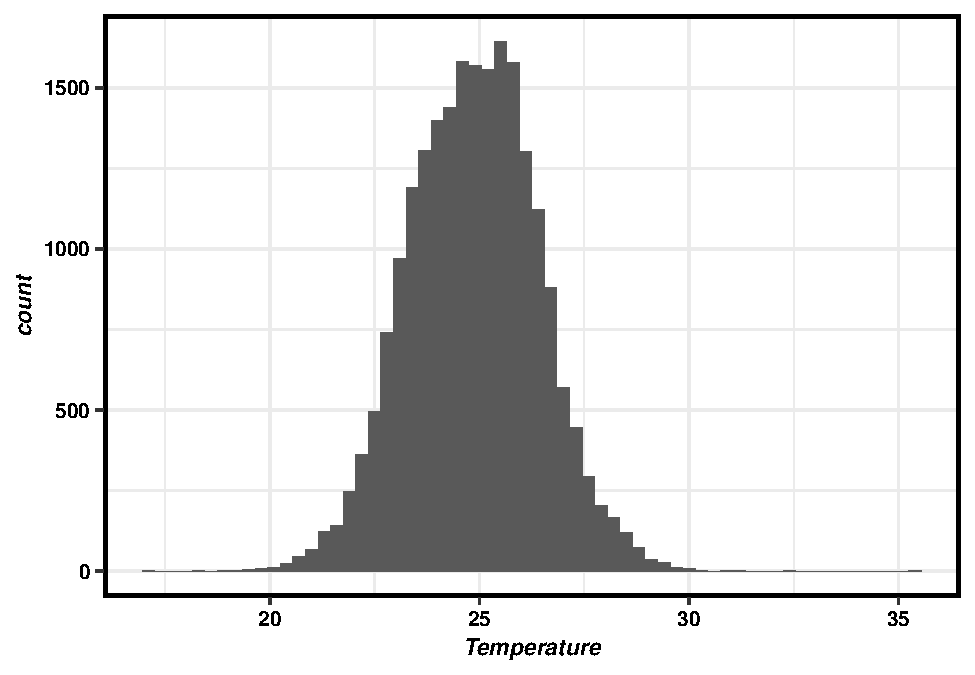
\includegraphics{Garcia_ENV872_Project_files/figure-latex/unnamed-chunk-21-1.pdf}

\subsection{QQNorm for Temperature}\label{qqnorm-for-temperature}

\begin{Shaded}
\begin{Highlighting}[]
 \KeywordTok{qqnorm}\NormalTok{(OahuDataClean2}\OperatorTok{$}\NormalTok{Temperature) }
\KeywordTok{qqline}\NormalTok{(OahuDataClean2}\OperatorTok{$}\NormalTok{Temperature)}
\end{Highlighting}
\end{Shaded}

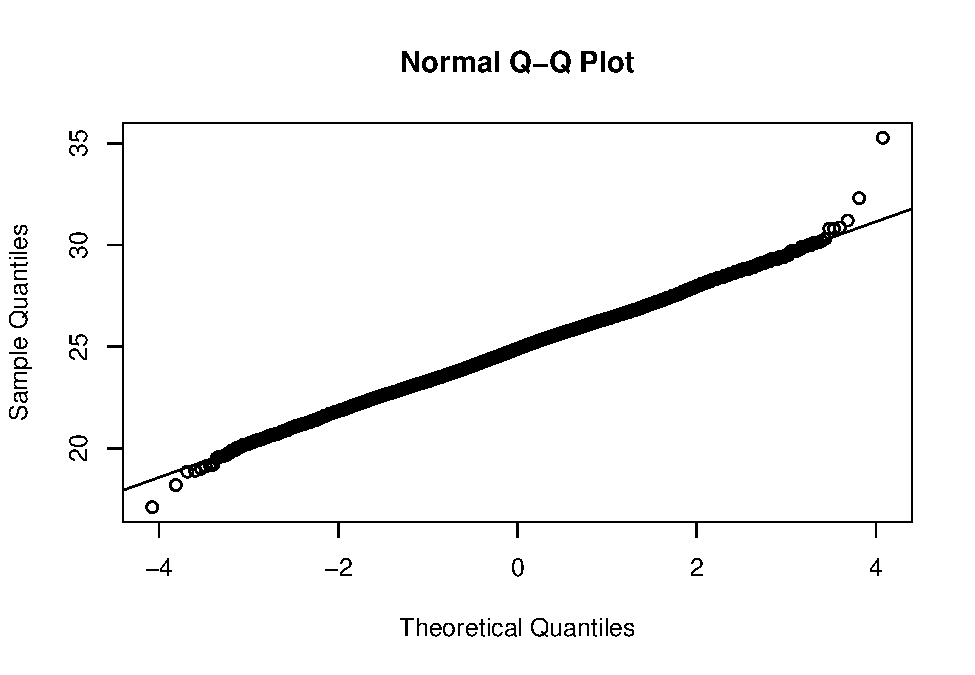
\includegraphics{Garcia_ENV872_Project_files/figure-latex/unnamed-chunk-22-1.pdf}

\subsection{LogTransform Temperature-doesn't look any
better}\label{logtransform-temperature-doesnt-look-any-better}

\begin{Shaded}
\begin{Highlighting}[]
\KeywordTok{qqnorm}\NormalTok{(}\KeywordTok{log}\NormalTok{(OahuDataClean2}\OperatorTok{$}\NormalTok{Temperature))}
\KeywordTok{qqline}\NormalTok{(}\KeywordTok{log}\NormalTok{(OahuDataClean2}\OperatorTok{$}\NormalTok{Temperature))}
\end{Highlighting}
\end{Shaded}

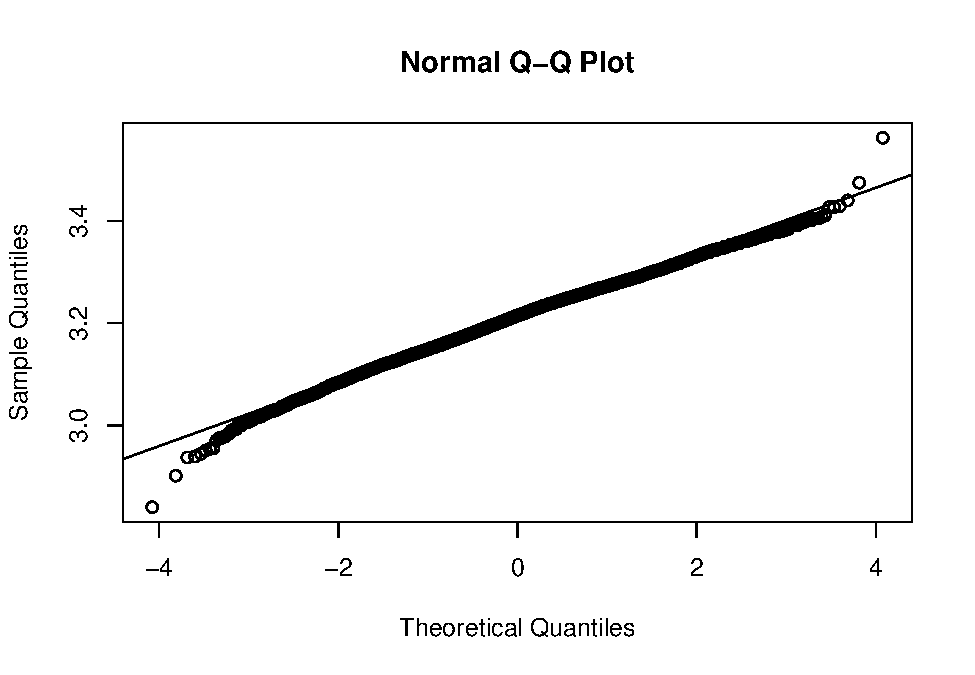
\includegraphics{Garcia_ENV872_Project_files/figure-latex/unnamed-chunk-23-1.pdf}

\subsection{Perform Shapiro Wilks Normality test for first 5,000
Temperature
observations}\label{perform-shapiro-wilks-normality-test-for-first-5000-temperature-observations}

\begin{Shaded}
\begin{Highlighting}[]
\KeywordTok{shapiro.test}\NormalTok{(OahuDataClean2}\OperatorTok{$}\NormalTok{Temperature[}\DecValTok{0}\OperatorTok{:}\DecValTok{5000}\NormalTok{])}
\end{Highlighting}
\end{Shaded}

\begin{verbatim}
## 
##  Shapiro-Wilk normality test
## 
## data:  OahuDataClean2$Temperature[0:5000]
## W = 0.99317, p-value = 9.529e-15
\end{verbatim}

\paragraph{Reject null hypothesis that Temperature is normally
distributed.}\label{reject-null-hypothesis-that-temperature-is-normally-distributed.}

\subsubsection{Summary of Temperature}\label{summary-of-temperature}

\begin{Shaded}
\begin{Highlighting}[]
\KeywordTok{summary}\NormalTok{(OahuDataClean2}\OperatorTok{$}\NormalTok{Temperature)}
\end{Highlighting}
\end{Shaded}

\begin{verbatim}
##    Min. 1st Qu.  Median    Mean 3rd Qu.    Max. 
##   17.11   23.80   24.90   24.87   25.92   35.27
\end{verbatim}

\subsection{Plot Temperature against
DO}\label{plot-temperature-against-do}

\begin{Shaded}
\begin{Highlighting}[]
\NormalTok{TempbyDO <-}\StringTok{ }
\StringTok{  }\KeywordTok{ggplot}\NormalTok{(OahuDataClean2, }\KeywordTok{aes}\NormalTok{(}\DataTypeTok{x =}\NormalTok{Temperature, }\DataTypeTok{y =}\NormalTok{DO)) }\OperatorTok{+}
\StringTok{  }\KeywordTok{geom_point}\NormalTok{(}\DataTypeTok{color=}\StringTok{"tomato3"}\NormalTok{, }\DataTypeTok{alpha=}\DecValTok{1}\NormalTok{, }\DataTypeTok{size=}\FloatTok{0.5}\NormalTok{) }\OperatorTok{+}
\StringTok{  }\KeywordTok{geom_smooth}\NormalTok{(}\DataTypeTok{method=}\NormalTok{lm, }\DataTypeTok{color=}\StringTok{"black"}\NormalTok{) }\OperatorTok{+}
\StringTok{  }\KeywordTok{labs}\NormalTok{(}\DataTypeTok{title=}\StringTok{"The Effect of Water Temperature on DO Concentrations across Oahu"}\NormalTok{, }\DataTypeTok{x=}\StringTok{"Water Temperature (degrees C)"}\NormalTok{, }\DataTypeTok{y=}\StringTok{"Dissolved Oxygen (mg/L)"}\NormalTok{)}
\KeywordTok{print}\NormalTok{(TempbyDO) }
\end{Highlighting}
\end{Shaded}

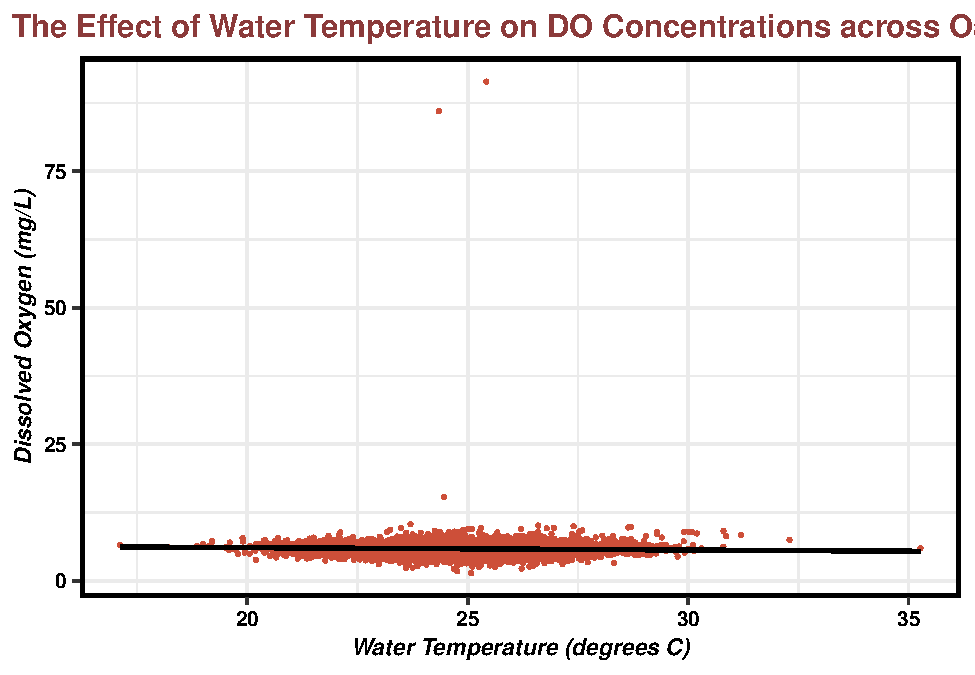
\includegraphics{Garcia_ENV872_Project_files/figure-latex/unnamed-chunk-26-1.pdf}

\subsection{pH}\label{ph}

\begin{Shaded}
\begin{Highlighting}[]
\KeywordTok{ggplot}\NormalTok{(OahuDataClean2) }\OperatorTok{+}
\StringTok{  }\KeywordTok{geom_histogram}\NormalTok{(}\KeywordTok{aes}\NormalTok{(}\DataTypeTok{x =}\NormalTok{pH))}\OperatorTok{+}
\StringTok{   }\KeywordTok{scale_x_continuous}\NormalTok{(}\DataTypeTok{limits =} \KeywordTok{c}\NormalTok{(}\DecValTok{0}\NormalTok{, }\DecValTok{12}\NormalTok{))}
\end{Highlighting}
\end{Shaded}

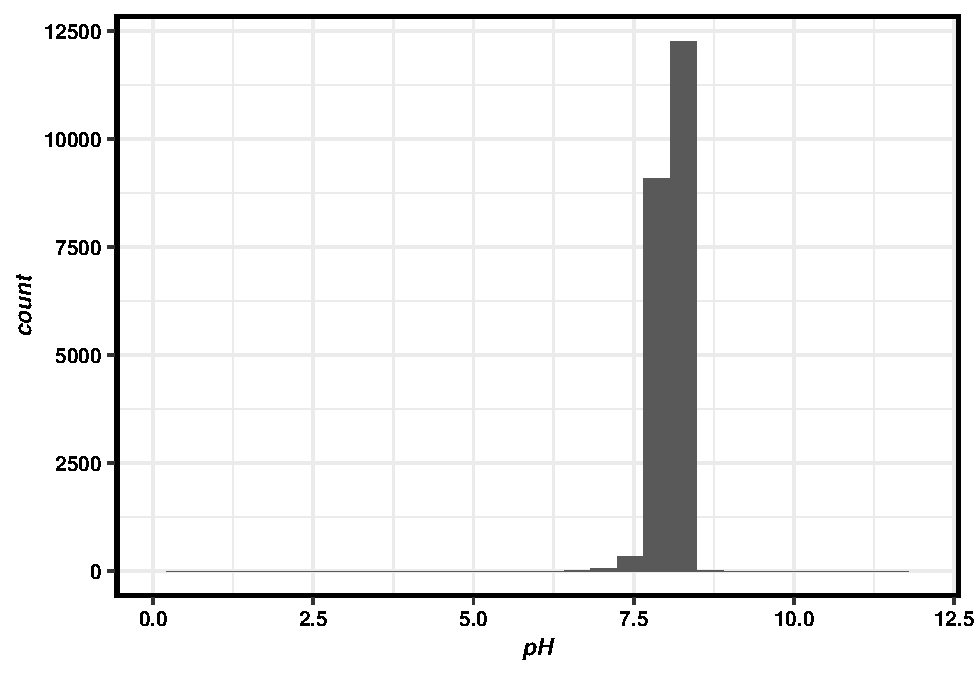
\includegraphics{Garcia_ENV872_Project_files/figure-latex/unnamed-chunk-27-1.pdf}

\subsection{QQNorm of pH}\label{qqnorm-of-ph}

\begin{Shaded}
\begin{Highlighting}[]
 \KeywordTok{qqnorm}\NormalTok{(OahuDataClean2}\OperatorTok{$}\NormalTok{pH) }
\KeywordTok{qqline}\NormalTok{(OahuDataClean2}\OperatorTok{$}\NormalTok{pH)}
\end{Highlighting}
\end{Shaded}

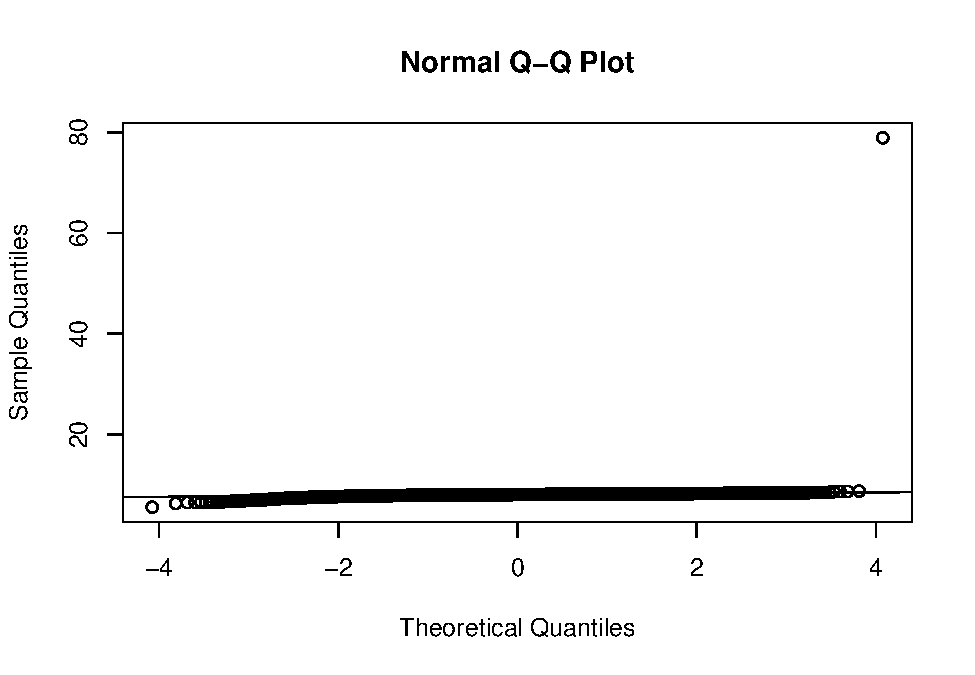
\includegraphics{Garcia_ENV872_Project_files/figure-latex/unnamed-chunk-28-1.pdf}

\subsection{Shapiro Wilks Test for pH}\label{shapiro-wilks-test-for-ph}

\begin{Shaded}
\begin{Highlighting}[]
\KeywordTok{shapiro.test}\NormalTok{(OahuDataClean2}\OperatorTok{$}\NormalTok{pH[}\DecValTok{0}\OperatorTok{:}\DecValTok{5000}\NormalTok{])}
\end{Highlighting}
\end{Shaded}

\begin{verbatim}
## 
##  Shapiro-Wilk normality test
## 
## data:  OahuDataClean2$pH[0:5000]
## W = 0.70546, p-value < 2.2e-16
\end{verbatim}

\subsubsection{Summary of pH}\label{summary-of-ph}

\begin{Shaded}
\begin{Highlighting}[]
\KeywordTok{summary}\NormalTok{(OahuDataClean2}\OperatorTok{$}\NormalTok{pH)}
\end{Highlighting}
\end{Shaded}

\begin{verbatim}
##    Min. 1st Qu.  Median    Mean 3rd Qu.    Max. 
##   5.570   8.000   8.080   8.064   8.150  78.900
\end{verbatim}

\subsubsection{Plot pH against DO}\label{plot-ph-against-do}

\begin{Shaded}
\begin{Highlighting}[]
\NormalTok{pHbyDO <-}\StringTok{ }
\StringTok{  }\KeywordTok{ggplot}\NormalTok{(OahuDataClean2, }\KeywordTok{aes}\NormalTok{(}\DataTypeTok{x =}\NormalTok{pH, }\DataTypeTok{y =}\NormalTok{DO)) }\OperatorTok{+}
\StringTok{  }\KeywordTok{geom_point}\NormalTok{(}\DataTypeTok{color=}\StringTok{"tomato3"}\NormalTok{, }\DataTypeTok{alpha=}\DecValTok{1}\NormalTok{, }\DataTypeTok{size=}\FloatTok{0.5}\NormalTok{) }\OperatorTok{+}
\StringTok{  }\KeywordTok{geom_smooth}\NormalTok{(}\DataTypeTok{method=}\NormalTok{lm, }\DataTypeTok{color=}\StringTok{"black"}\NormalTok{, }\DataTypeTok{se=}\OtherTok{FALSE}\NormalTok{) }\OperatorTok{+}
\StringTok{  }\KeywordTok{labs}\NormalTok{(}\DataTypeTok{title=}\StringTok{"The Effect of pH on DO Concentrations across Oahu"}\NormalTok{, }\DataTypeTok{x=}\StringTok{"pH"}\NormalTok{, }\DataTypeTok{y=}\StringTok{"Dissolved Oxygen (mg/L)"}\NormalTok{)}\OperatorTok{+}
\StringTok{   }\KeywordTok{scale_x_continuous}\NormalTok{(}\DataTypeTok{limits =} \KeywordTok{c}\NormalTok{(}\DecValTok{0}\NormalTok{, }\DecValTok{12}\NormalTok{))}
\KeywordTok{print}\NormalTok{(pHbyDO) }
\end{Highlighting}
\end{Shaded}

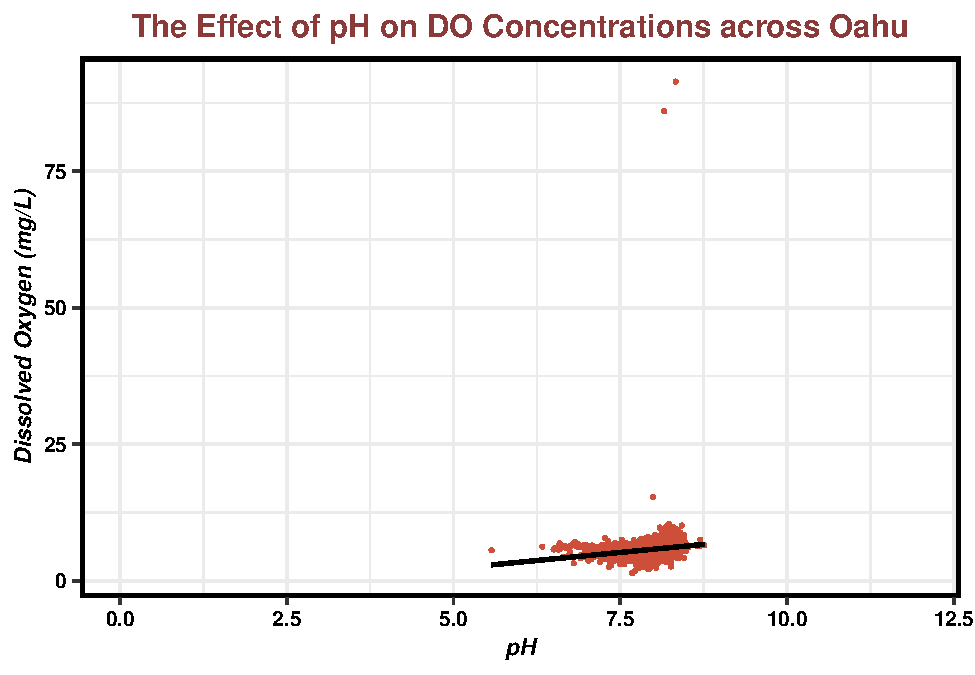
\includegraphics{Garcia_ENV872_Project_files/figure-latex/unnamed-chunk-31-1.pdf}

\subsection{Dissolved Oxygen
Concentrations}\label{dissolved-oxygen-concentrations}

\begin{Shaded}
\begin{Highlighting}[]
\KeywordTok{ggplot}\NormalTok{(OahuDataClean2) }\OperatorTok{+}
\StringTok{  }\KeywordTok{geom_histogram}\NormalTok{(}\KeywordTok{aes}\NormalTok{(}\DataTypeTok{x =}\NormalTok{DO)) }\OperatorTok{+}
\KeywordTok{scale_x_continuous}\NormalTok{(}\DataTypeTok{limits =} \KeywordTok{c}\NormalTok{(}\DecValTok{0}\NormalTok{, }\DecValTok{15}\NormalTok{))}
\end{Highlighting}
\end{Shaded}

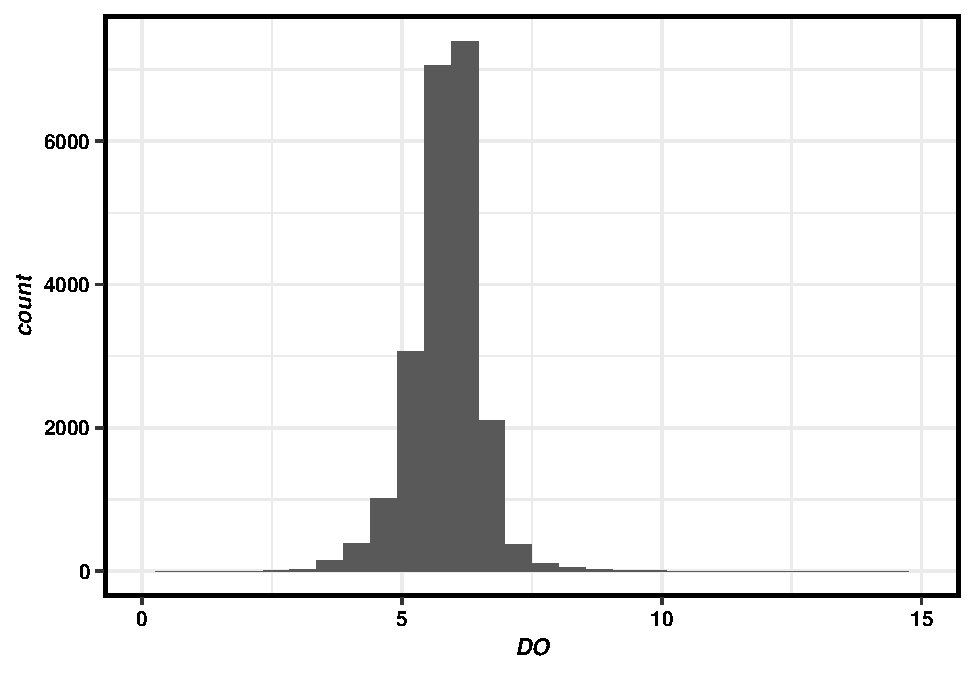
\includegraphics{Garcia_ENV872_Project_files/figure-latex/unnamed-chunk-32-1.pdf}

\subsection{QQNorm of DO}\label{qqnorm-of-do}

\begin{Shaded}
\begin{Highlighting}[]
 \KeywordTok{qqnorm}\NormalTok{(OahuDataClean2}\OperatorTok{$}\NormalTok{DO) }
\KeywordTok{qqline}\NormalTok{(OahuDataClean2}\OperatorTok{$}\NormalTok{DO)}
\end{Highlighting}
\end{Shaded}

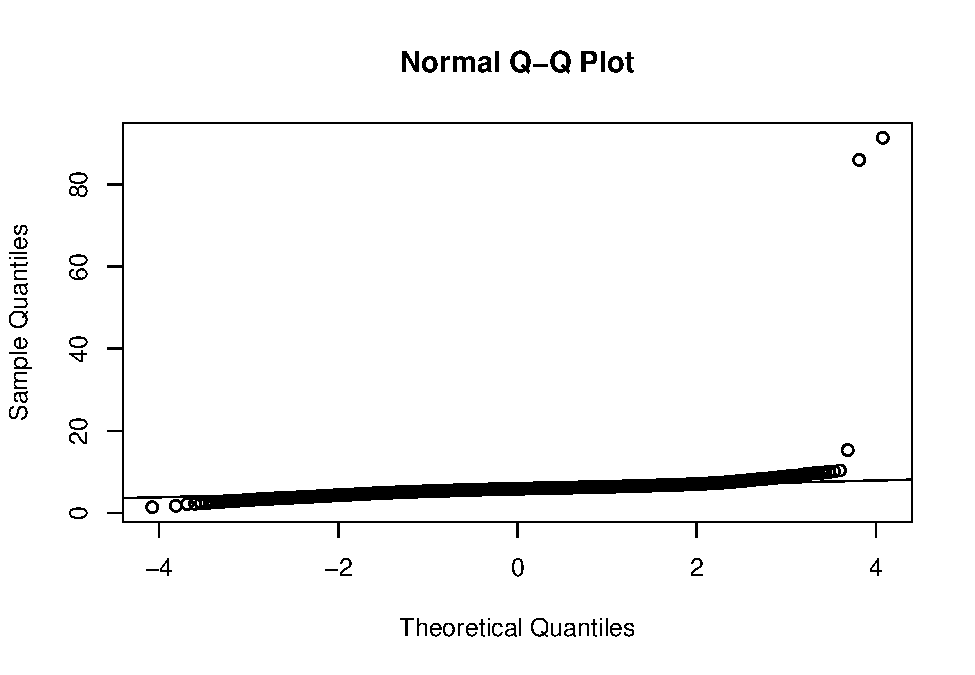
\includegraphics{Garcia_ENV872_Project_files/figure-latex/unnamed-chunk-33-1.pdf}

\subsubsection{Shapiro Wilks Test for
DO}\label{shapiro-wilks-test-for-do}

\begin{Shaded}
\begin{Highlighting}[]
\KeywordTok{shapiro.test}\NormalTok{(OahuDataClean2}\OperatorTok{$}\NormalTok{DO[}\DecValTok{0}\OperatorTok{:}\DecValTok{5000}\NormalTok{])}
\end{Highlighting}
\end{Shaded}

\begin{verbatim}
## 
##  Shapiro-Wilk normality test
## 
## data:  OahuDataClean2$DO[0:5000]
## W = 0.9109, p-value < 2.2e-16
\end{verbatim}

\subsection{Summary of DO}\label{summary-of-do}

\begin{Shaded}
\begin{Highlighting}[]
\KeywordTok{summary}\NormalTok{(OahuDataClean2}\OperatorTok{$}\NormalTok{DO)}
\end{Highlighting}
\end{Shaded}

\begin{verbatim}
##    Min. 1st Qu.  Median    Mean 3rd Qu.    Max. 
##   1.400   5.520   5.900   5.857   6.210  91.400
\end{verbatim}

\subsection{Percent Saturation of Dissolved
Oxygen}\label{percent-saturation-of-dissolved-oxygen}

\begin{Shaded}
\begin{Highlighting}[]
\KeywordTok{ggplot}\NormalTok{(OahuDataClean2) }\OperatorTok{+}
\StringTok{  }\KeywordTok{geom_histogram}\NormalTok{(}\KeywordTok{aes}\NormalTok{(}\DataTypeTok{x =}\NormalTok{DissolvedOxygenSaturation))}
\end{Highlighting}
\end{Shaded}

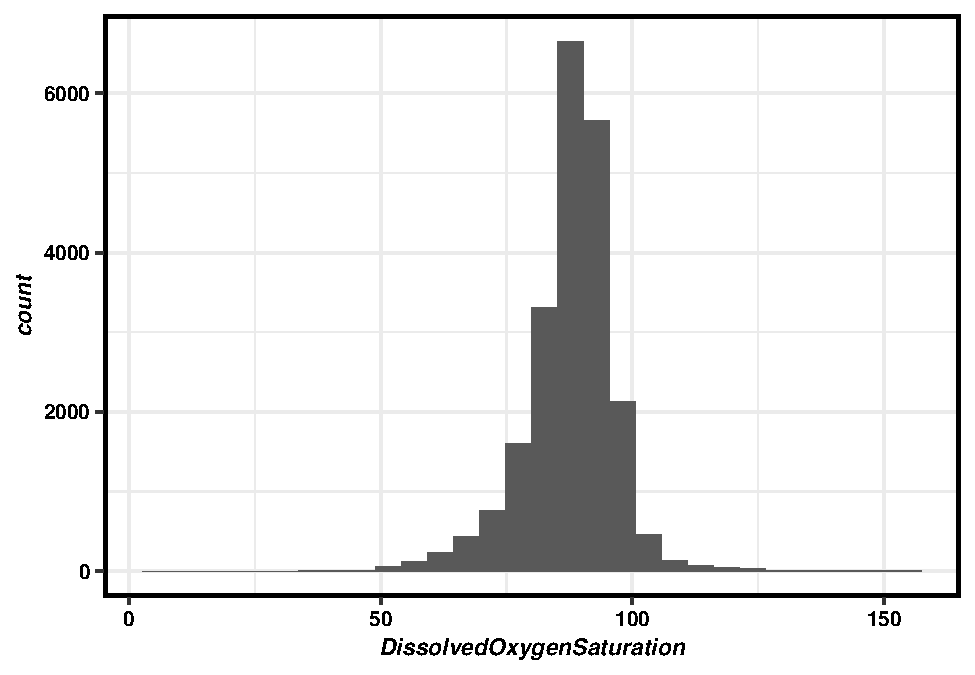
\includegraphics{Garcia_ENV872_Project_files/figure-latex/unnamed-chunk-36-1.pdf}

\subsection{QQnorm of Percent Saturation of Dissolved
Oxygen}\label{qqnorm-of-percent-saturation-of-dissolved-oxygen}

\begin{Shaded}
\begin{Highlighting}[]
\KeywordTok{qqnorm}\NormalTok{(OahuDataClean2}\OperatorTok{$}\NormalTok{DissolvedOxygenSaturation) }
\KeywordTok{qqline}\NormalTok{(OahuDataClean2}\OperatorTok{$}\NormalTok{DissolvedOxygenSaturation)}
\end{Highlighting}
\end{Shaded}

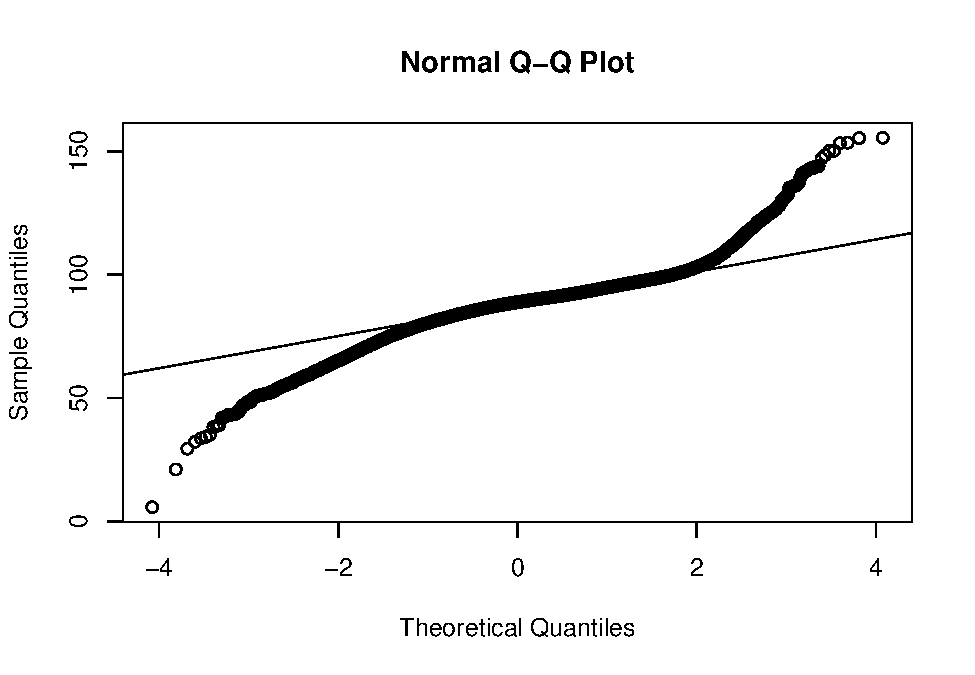
\includegraphics{Garcia_ENV872_Project_files/figure-latex/unnamed-chunk-37-1.pdf}

\subsection{Shapiro Test for Percent Saturation Dissolved
Oxygen}\label{shapiro-test-for-percent-saturation-dissolved-oxygen}

\begin{Shaded}
\begin{Highlighting}[]
\KeywordTok{shapiro.test}\NormalTok{(OahuDataClean2}\OperatorTok{$}\NormalTok{DissolvedOxygenSaturation[}\DecValTok{0}\OperatorTok{:}\DecValTok{5000}\NormalTok{])}
\end{Highlighting}
\end{Shaded}

\begin{verbatim}
## 
##  Shapiro-Wilk normality test
## 
## data:  OahuDataClean2$DissolvedOxygenSaturation[0:5000]
## W = 0.87819, p-value < 2.2e-16
\end{verbatim}

\subsubsection{Summary of Percent Saturation of Dissolved
Oxygen}\label{summary-of-percent-saturation-of-dissolved-oxygen}

\begin{Shaded}
\begin{Highlighting}[]
\KeywordTok{summary}\NormalTok{(OahuDataClean2}\OperatorTok{$}\NormalTok{DissolvedOxygenSaturation)}
\end{Highlighting}
\end{Shaded}

\begin{verbatim}
##    Min. 1st Qu.  Median    Mean 3rd Qu.    Max. 
##    5.79   83.80   88.90   87.76   92.60  155.50
\end{verbatim}

\subsection{Turbidity}\label{turbidity}

\begin{Shaded}
\begin{Highlighting}[]
\KeywordTok{ggplot}\NormalTok{(OahuDataClean2) }\OperatorTok{+}
\StringTok{  }\KeywordTok{geom_histogram}\NormalTok{(}\KeywordTok{aes}\NormalTok{(}\DataTypeTok{x =}\NormalTok{Turbidity)) }\OperatorTok{+}
\StringTok{   }\KeywordTok{scale_x_continuous}\NormalTok{(}\DataTypeTok{limits =} \KeywordTok{c}\NormalTok{(}\DecValTok{0}\NormalTok{, }\DecValTok{100}\NormalTok{))}
\end{Highlighting}
\end{Shaded}

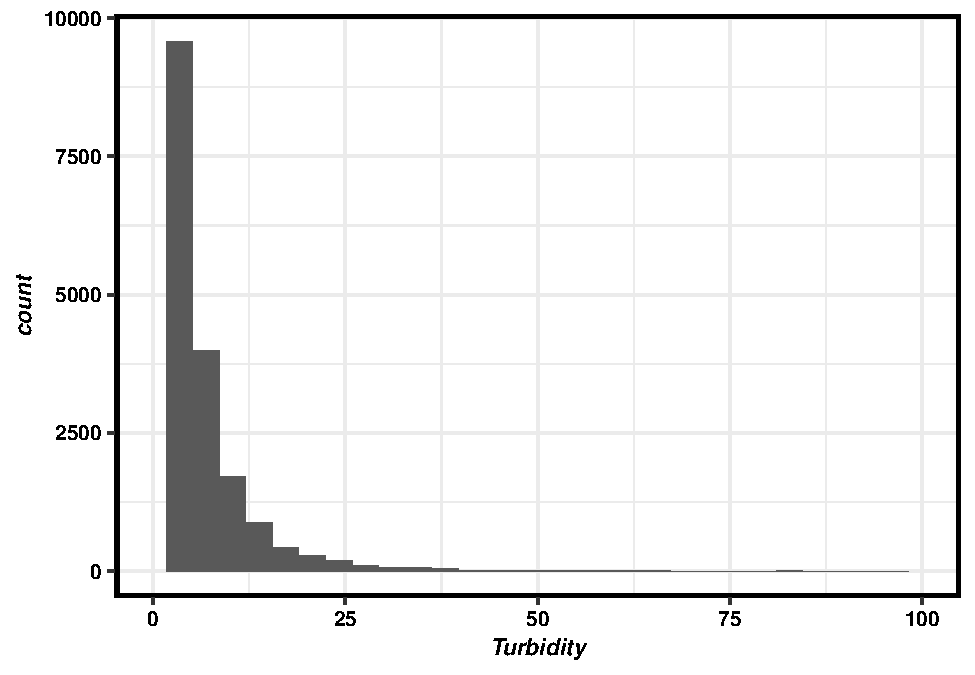
\includegraphics{Garcia_ENV872_Project_files/figure-latex/unnamed-chunk-40-1.pdf}

\subsection{QQNorm of Turbidity}\label{qqnorm-of-turbidity}

\begin{Shaded}
\begin{Highlighting}[]
\KeywordTok{qqnorm}\NormalTok{(OahuDataClean2}\OperatorTok{$}\NormalTok{Turbidity) }
\KeywordTok{qqline}\NormalTok{(OahuDataClean2}\OperatorTok{$}\NormalTok{Turbidity)}
\end{Highlighting}
\end{Shaded}

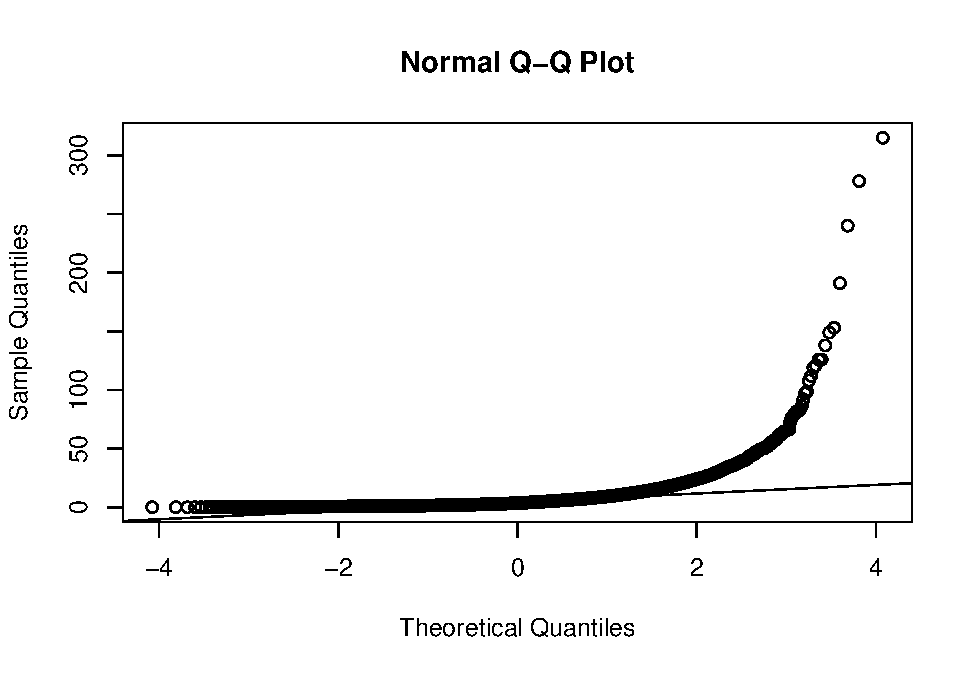
\includegraphics{Garcia_ENV872_Project_files/figure-latex/unnamed-chunk-41-1.pdf}

\subsubsection{Shapiro Test for
Turbidity}\label{shapiro-test-for-turbidity}

\begin{Shaded}
\begin{Highlighting}[]
\KeywordTok{shapiro.test}\NormalTok{(OahuDataClean2}\OperatorTok{$}\NormalTok{Turbidity[}\DecValTok{0}\OperatorTok{:}\DecValTok{5000}\NormalTok{])}
\end{Highlighting}
\end{Shaded}

\begin{verbatim}
## 
##  Shapiro-Wilk normality test
## 
## data:  OahuDataClean2$Turbidity[0:5000]
## W = 0.65218, p-value < 2.2e-16
\end{verbatim}

\subsubsection{Summary of Turbidity}\label{summary-of-turbidity}

\begin{Shaded}
\begin{Highlighting}[]
\KeywordTok{summary}\NormalTok{(OahuDataClean2}\OperatorTok{$}\NormalTok{Turbidity)}
\end{Highlighting}
\end{Shaded}

\begin{verbatim}
##    Min. 1st Qu.  Median    Mean 3rd Qu.    Max. 
##   0.100   1.990   3.640   5.779   6.930 315.000
\end{verbatim}

\subsection{Plot Turbidity against DO}\label{plot-turbidity-against-do}

\begin{Shaded}
\begin{Highlighting}[]
\NormalTok{TurbiditybyDO <-}\StringTok{ }
\StringTok{  }\KeywordTok{ggplot}\NormalTok{(OahuDataClean2, }\KeywordTok{aes}\NormalTok{(}\DataTypeTok{x =}\NormalTok{Turbidity, }\DataTypeTok{y =}\NormalTok{DO)) }\OperatorTok{+}
\StringTok{  }\KeywordTok{geom_point}\NormalTok{(}\DataTypeTok{color=}\StringTok{"tomato3"}\NormalTok{, }\DataTypeTok{alpha=}\DecValTok{1}\NormalTok{, }\DataTypeTok{size=}\FloatTok{0.5}\NormalTok{) }\OperatorTok{+}
\StringTok{  }\KeywordTok{geom_smooth}\NormalTok{(}\DataTypeTok{method=}\StringTok{"lm"}\NormalTok{, }\DataTypeTok{se=}\OtherTok{FALSE}\NormalTok{) }\OperatorTok{+}
\StringTok{   }\KeywordTok{scale_y_continuous}\NormalTok{(}\DataTypeTok{limits =} \KeywordTok{c}\NormalTok{(}\DecValTok{0}\NormalTok{, }\DecValTok{25}\NormalTok{)) }\OperatorTok{+}
\StringTok{  }
\StringTok{  }\KeywordTok{labs}\NormalTok{(}\DataTypeTok{title=}\StringTok{"The Effect of Turbidity on DO Concentrations across Oahu"}\NormalTok{, }\DataTypeTok{x=}\StringTok{"Turbidity (NTU)"}\NormalTok{, }\DataTypeTok{y=}\StringTok{"Dissolved Oxygen (mg/L)"}\NormalTok{)}
\KeywordTok{print}\NormalTok{(TurbiditybyDO) }
\end{Highlighting}
\end{Shaded}

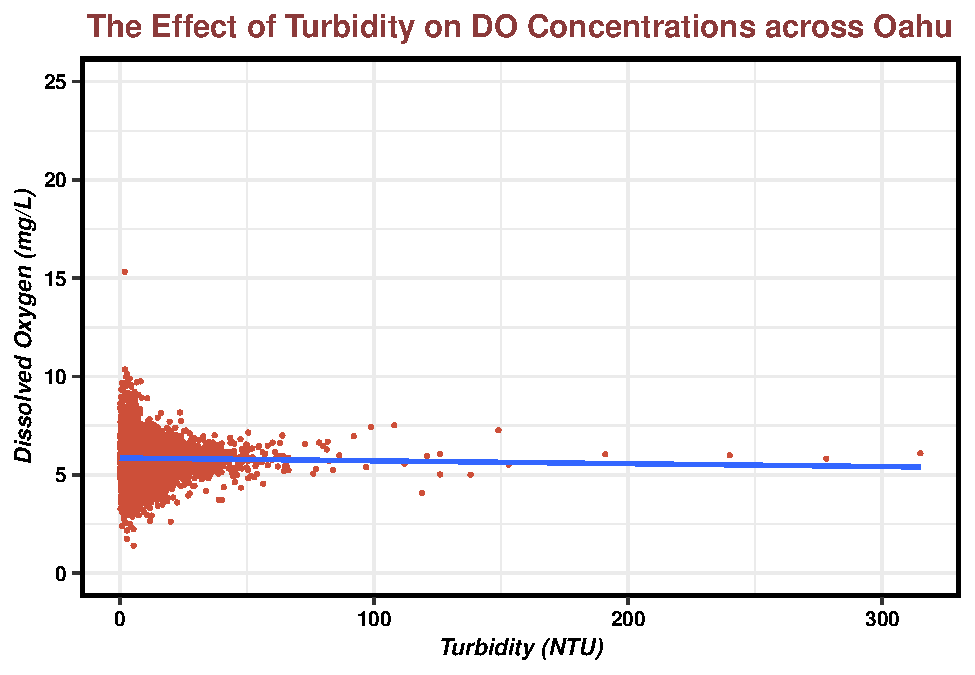
\includegraphics{Garcia_ENV872_Project_files/figure-latex/unnamed-chunk-44-1.pdf}

\subsection{Salinity}\label{salinity}

\begin{Shaded}
\begin{Highlighting}[]
\KeywordTok{ggplot}\NormalTok{(OahuDataClean2) }\OperatorTok{+}
\StringTok{  }\KeywordTok{geom_histogram}\NormalTok{(}\KeywordTok{aes}\NormalTok{(}\DataTypeTok{x =}\NormalTok{Salinity))}
\end{Highlighting}
\end{Shaded}

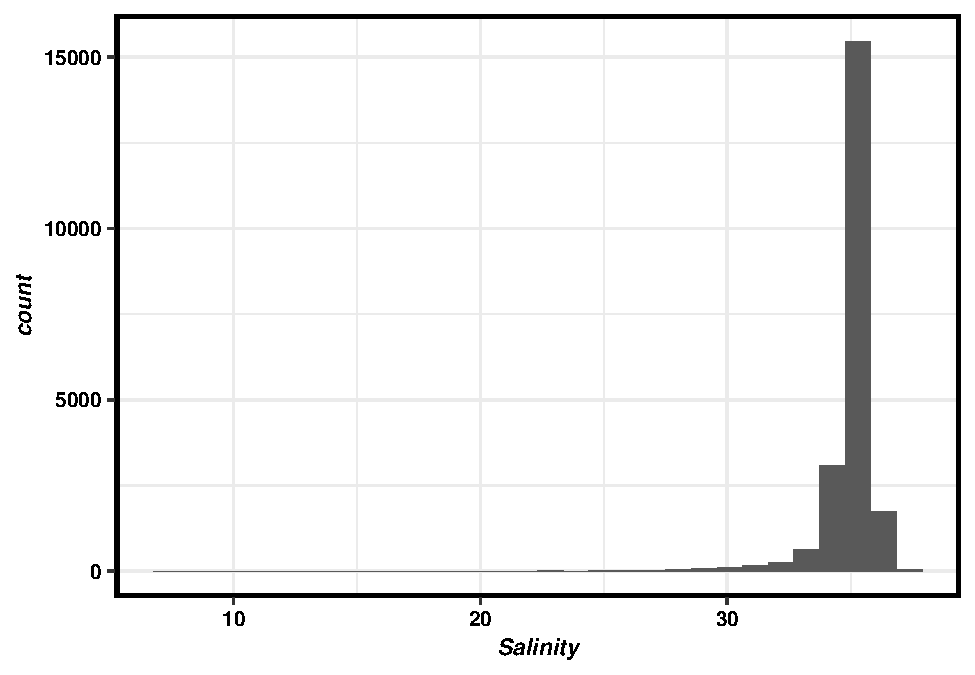
\includegraphics{Garcia_ENV872_Project_files/figure-latex/unnamed-chunk-45-1.pdf}

\subsection{QQNorm of Salinity}\label{qqnorm-of-salinity}

\begin{Shaded}
\begin{Highlighting}[]
\KeywordTok{qqnorm}\NormalTok{(OahuDataClean2}\OperatorTok{$}\NormalTok{Salinity) }
\KeywordTok{qqline}\NormalTok{(OahuDataClean2}\OperatorTok{$}\NormalTok{Salinity)}
\end{Highlighting}
\end{Shaded}

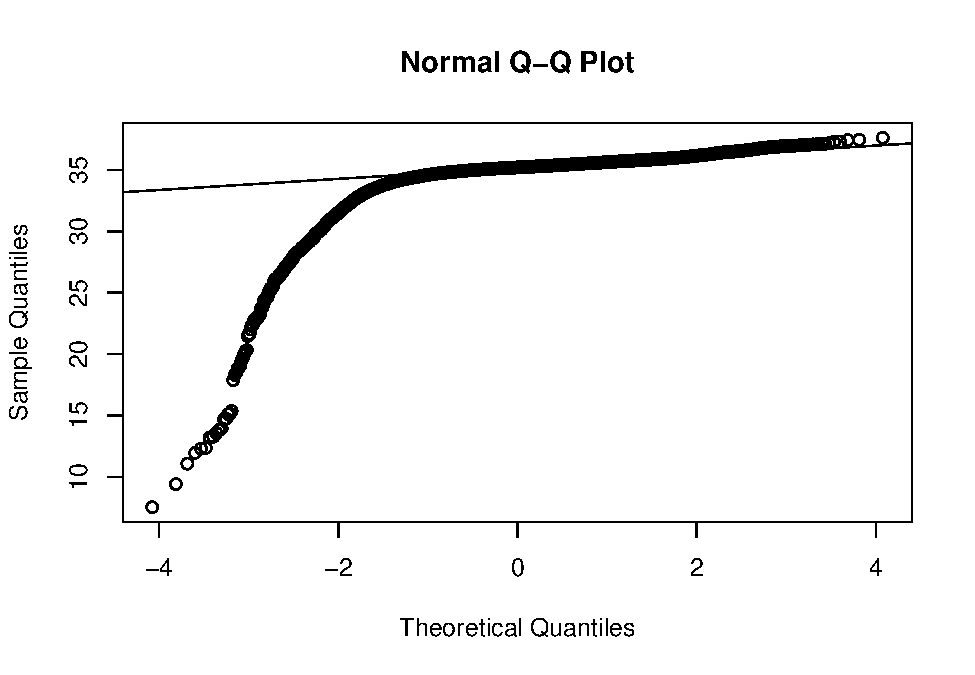
\includegraphics{Garcia_ENV872_Project_files/figure-latex/unnamed-chunk-46-1.pdf}

\subsection{Shapiro Test for Salinity}\label{shapiro-test-for-salinity}

\begin{Shaded}
\begin{Highlighting}[]
\KeywordTok{shapiro.test}\NormalTok{(OahuDataClean2}\OperatorTok{$}\NormalTok{Salinity[}\DecValTok{0}\OperatorTok{:}\DecValTok{5000}\NormalTok{])}
\end{Highlighting}
\end{Shaded}

\begin{verbatim}
## 
##  Shapiro-Wilk normality test
## 
## data:  OahuDataClean2$Salinity[0:5000]
## W = 0.52773, p-value < 2.2e-16
\end{verbatim}

\subsubsection{Summary of Salinity}\label{summary-of-salinity}

\begin{Shaded}
\begin{Highlighting}[]
\KeywordTok{summary}\NormalTok{(OahuDataClean2}\OperatorTok{$}\NormalTok{Salinity)}
\end{Highlighting}
\end{Shaded}

\begin{verbatim}
##    Min. 1st Qu.  Median    Mean 3rd Qu.    Max. 
##    7.52   34.87   35.20   34.96   35.48   37.62
\end{verbatim}

\subsection{Plot Salinity Against DO}\label{plot-salinity-against-do}

\begin{Shaded}
\begin{Highlighting}[]
\NormalTok{SalinitybyDO <-}\StringTok{ }
\StringTok{  }\KeywordTok{ggplot}\NormalTok{(OahuDataClean2, }\KeywordTok{aes}\NormalTok{(}\DataTypeTok{x =}\NormalTok{Salinity, }\DataTypeTok{y =}\NormalTok{DO)) }\OperatorTok{+}
\StringTok{  }\KeywordTok{geom_point}\NormalTok{(}\DataTypeTok{color=}\StringTok{"tomato3"}\NormalTok{, }\DataTypeTok{alpha=}\DecValTok{1}\NormalTok{, }\DataTypeTok{size=}\FloatTok{0.5}\NormalTok{) }\OperatorTok{+}
\StringTok{  }\KeywordTok{geom_smooth}\NormalTok{(}\DataTypeTok{method=}\NormalTok{lm, }\DataTypeTok{color=}\StringTok{"black"}\NormalTok{, }\DataTypeTok{se=}\OtherTok{FALSE}\NormalTok{) }\OperatorTok{+}
\StringTok{  }\KeywordTok{labs}\NormalTok{(}\DataTypeTok{title=}\StringTok{"The Effect of Salinity on DO Concentrations across Oahu"}\NormalTok{, }\DataTypeTok{x=}\StringTok{"Salinity (ppt)"}\NormalTok{, }\DataTypeTok{y=}\StringTok{"Dissolved Oxygen (mg/L)"}\NormalTok{)}
\KeywordTok{print}\NormalTok{(SalinitybyDO) }
\end{Highlighting}
\end{Shaded}

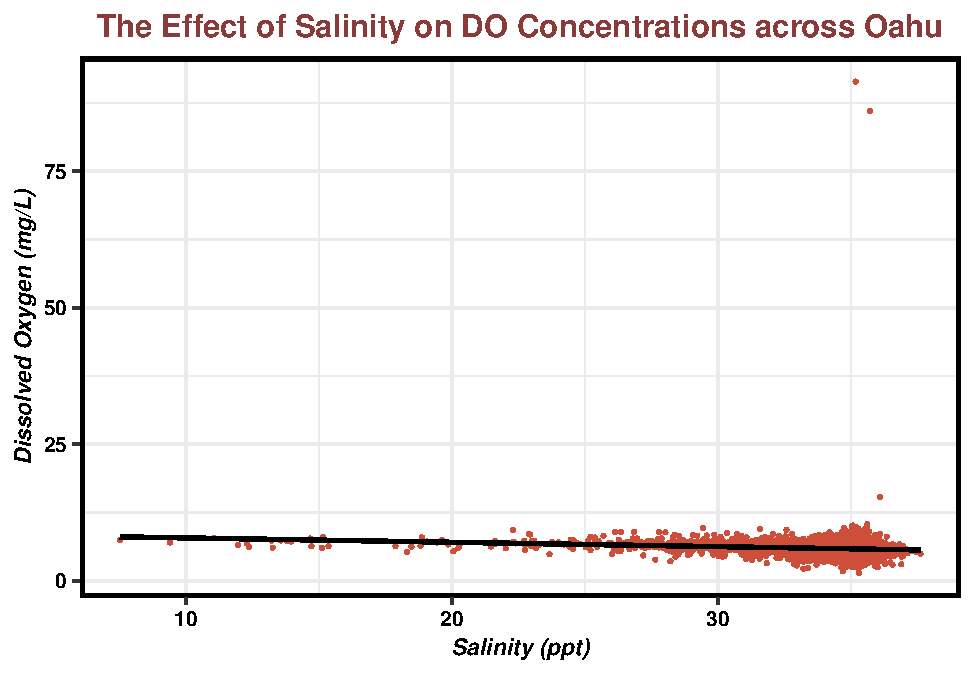
\includegraphics{Garcia_ENV872_Project_files/figure-latex/unnamed-chunk-49-1.pdf}

\subsection{Enterococcus}\label{enterococcus}

\begin{Shaded}
\begin{Highlighting}[]
\KeywordTok{ggplot}\NormalTok{(OahuDataClean2) }\OperatorTok{+}
\StringTok{  }\KeywordTok{geom_histogram}\NormalTok{(}\KeywordTok{aes}\NormalTok{(}\DataTypeTok{x =}\NormalTok{Enterococcus))}
\end{Highlighting}
\end{Shaded}

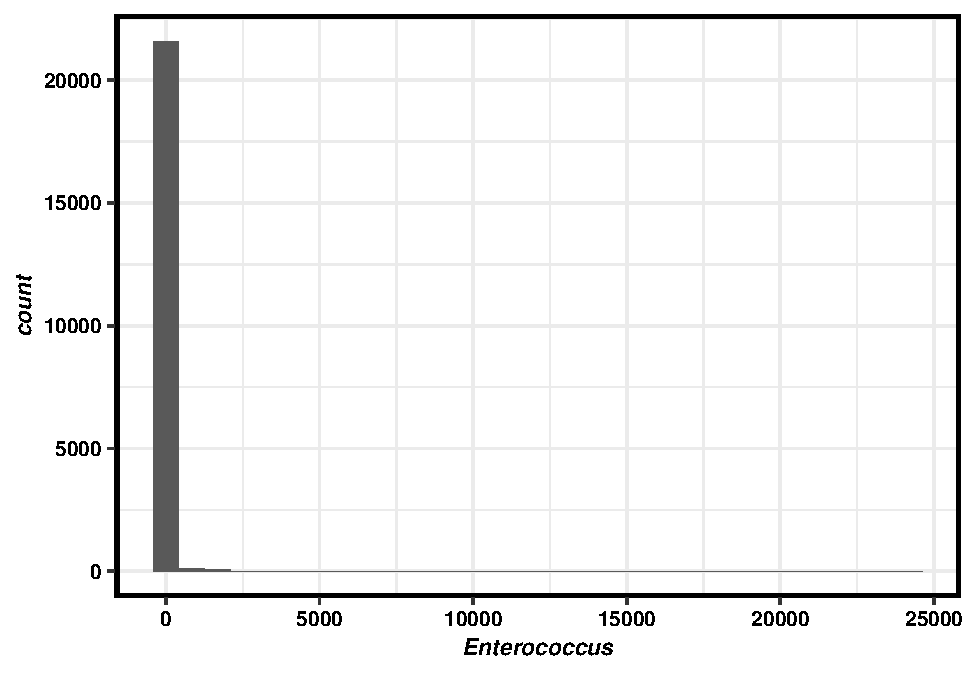
\includegraphics{Garcia_ENV872_Project_files/figure-latex/unnamed-chunk-50-1.pdf}

\subsection{QQNorm of Enterococcus}\label{qqnorm-of-enterococcus}

\begin{Shaded}
\begin{Highlighting}[]
\KeywordTok{qqnorm}\NormalTok{(OahuDataClean2}\OperatorTok{$}\NormalTok{Enterococcus) }
\KeywordTok{qqline}\NormalTok{(OahuDataClean2}\OperatorTok{$}\NormalTok{Enterococcus)}
\end{Highlighting}
\end{Shaded}

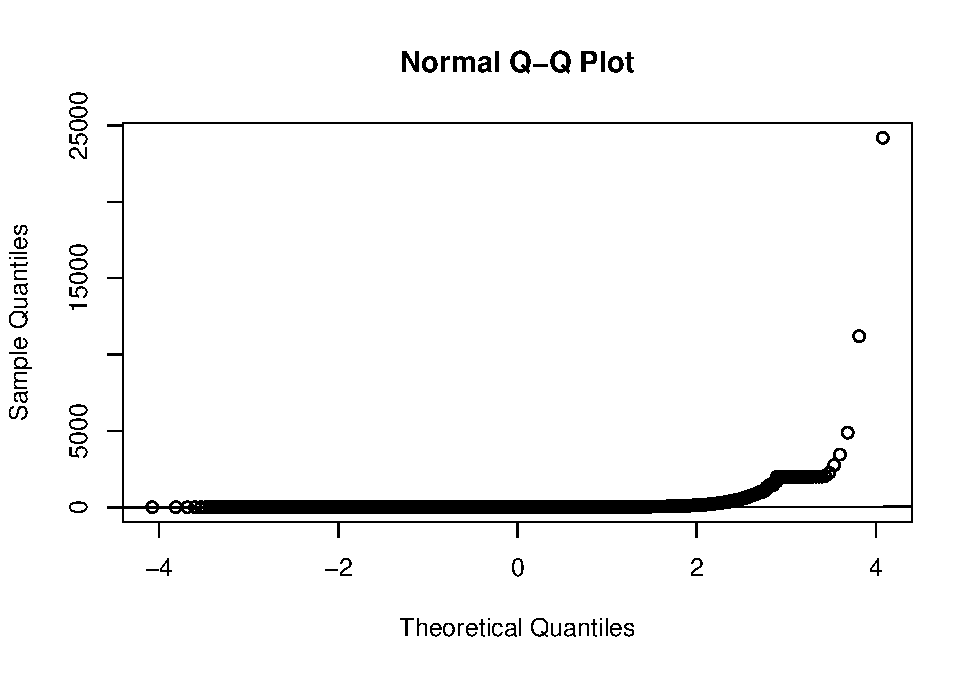
\includegraphics{Garcia_ENV872_Project_files/figure-latex/unnamed-chunk-51-1.pdf}

\subsection{Shapiro Test for
Enterococcus}\label{shapiro-test-for-enterococcus}

\begin{Shaded}
\begin{Highlighting}[]
\KeywordTok{shapiro.test}\NormalTok{(OahuDataClean2}\OperatorTok{$}\NormalTok{Enterococcus[}\DecValTok{0}\OperatorTok{:}\DecValTok{5000}\NormalTok{])}
\end{Highlighting}
\end{Shaded}

\begin{verbatim}
## 
##  Shapiro-Wilk normality test
## 
## data:  OahuDataClean2$Enterococcus[0:5000]
## W = 0.027629, p-value < 2.2e-16
\end{verbatim}

\subsection{Summary of Enterococcus}\label{summary-of-enterococcus}

\begin{Shaded}
\begin{Highlighting}[]
\KeywordTok{summary}\NormalTok{(OahuDataClean2}\OperatorTok{$}\NormalTok{Enterococcus)}
\end{Highlighting}
\end{Shaded}

\begin{verbatim}
##     Min.  1st Qu.   Median     Mean  3rd Qu.     Max. 
##     0.30     2.30     2.30    22.84    10.00 24196.00
\end{verbatim}

\subsubsection{Convert Date Column to a Date
Object}\label{convert-date-column-to-a-date-object}

\begin{Shaded}
\begin{Highlighting}[]
\NormalTok{OahuDataClean2}\OperatorTok{$}\NormalTok{Date<-}\KeywordTok{as.Date}\NormalTok{(OahuDataClean2}\OperatorTok{$}\NormalTok{Date, }\DataTypeTok{format=}\StringTok{"%m/%d/%y"}\NormalTok{)}
\end{Highlighting}
\end{Shaded}

\section{Correlation Plot of Data}\label{correlation-plot-of-data}

\begin{Shaded}
\begin{Highlighting}[]
\KeywordTok{ggpairs}\NormalTok{(OahuDataClean, }\DataTypeTok{columns=}\KeywordTok{c}\NormalTok{(}\DecValTok{9}\NormalTok{, }\DecValTok{13}\OperatorTok{:}\DecValTok{18}\NormalTok{), }\DataTypeTok{title=}\StringTok{"Correlation Plot of Oahu Water Quality Parameters"}\NormalTok{)}
\end{Highlighting}
\end{Shaded}

\includegraphics{Garcia_ENV872_Project_files/figure-latex/unnamed-chunk-55-1.pdf}

\section{Exploratory Boxplot showing Range of DO Concentrations by
Region in
Oahu}\label{exploratory-boxplot-showing-range-of-do-concentrations-by-region-in-oahu}

\begin{Shaded}
\begin{Highlighting}[]
\NormalTok{DOBoxplot<-}\KeywordTok{ggplot}\NormalTok{(OahuDataClean) }\OperatorTok{+}\StringTok{ }
\StringTok{  }\KeywordTok{geom_boxplot}\NormalTok{(}\KeywordTok{aes}\NormalTok{(}\DataTypeTok{x=}\NormalTok{Region, }\DataTypeTok{y=}\NormalTok{DO, }\DataTypeTok{fill=}\NormalTok{Region))  }\OperatorTok{+}
\StringTok{  }\KeywordTok{labs}\NormalTok{(}\DataTypeTok{title=}\StringTok{"Effect of Region on Range of Dissolved Oxygen Concentrations in Oahu"}\NormalTok{, }\DataTypeTok{x=}\StringTok{"Region in Oahu"}\NormalTok{, }\DataTypeTok{y=}\StringTok{"Dissolved Oxygen Concentration (mg/L)"}\NormalTok{) }\OperatorTok{+}
\KeywordTok{theme}\NormalTok{(}\DataTypeTok{legend.title =} \KeywordTok{element_text}\NormalTok{(}\DataTypeTok{colour=}\StringTok{"IndianRed"}\NormalTok{, }\DataTypeTok{size=}\DecValTok{16}\NormalTok{, }\DataTypeTok{face=}\StringTok{"bold"}\NormalTok{)) }\OperatorTok{+}\NormalTok{gabytheme }\OperatorTok{+}
\KeywordTok{scale_fill_brewer}\NormalTok{(}\DataTypeTok{palette=}\StringTok{"Set3"}\NormalTok{) }\OperatorTok{+}
\StringTok{  }\KeywordTok{scale_y_continuous}\NormalTok{(}\DataTypeTok{limits =} \KeywordTok{c}\NormalTok{(}\DecValTok{0}\NormalTok{, }\DecValTok{12}\NormalTok{))}
 \KeywordTok{print}\NormalTok{(DOBoxplot)}
\end{Highlighting}
\end{Shaded}

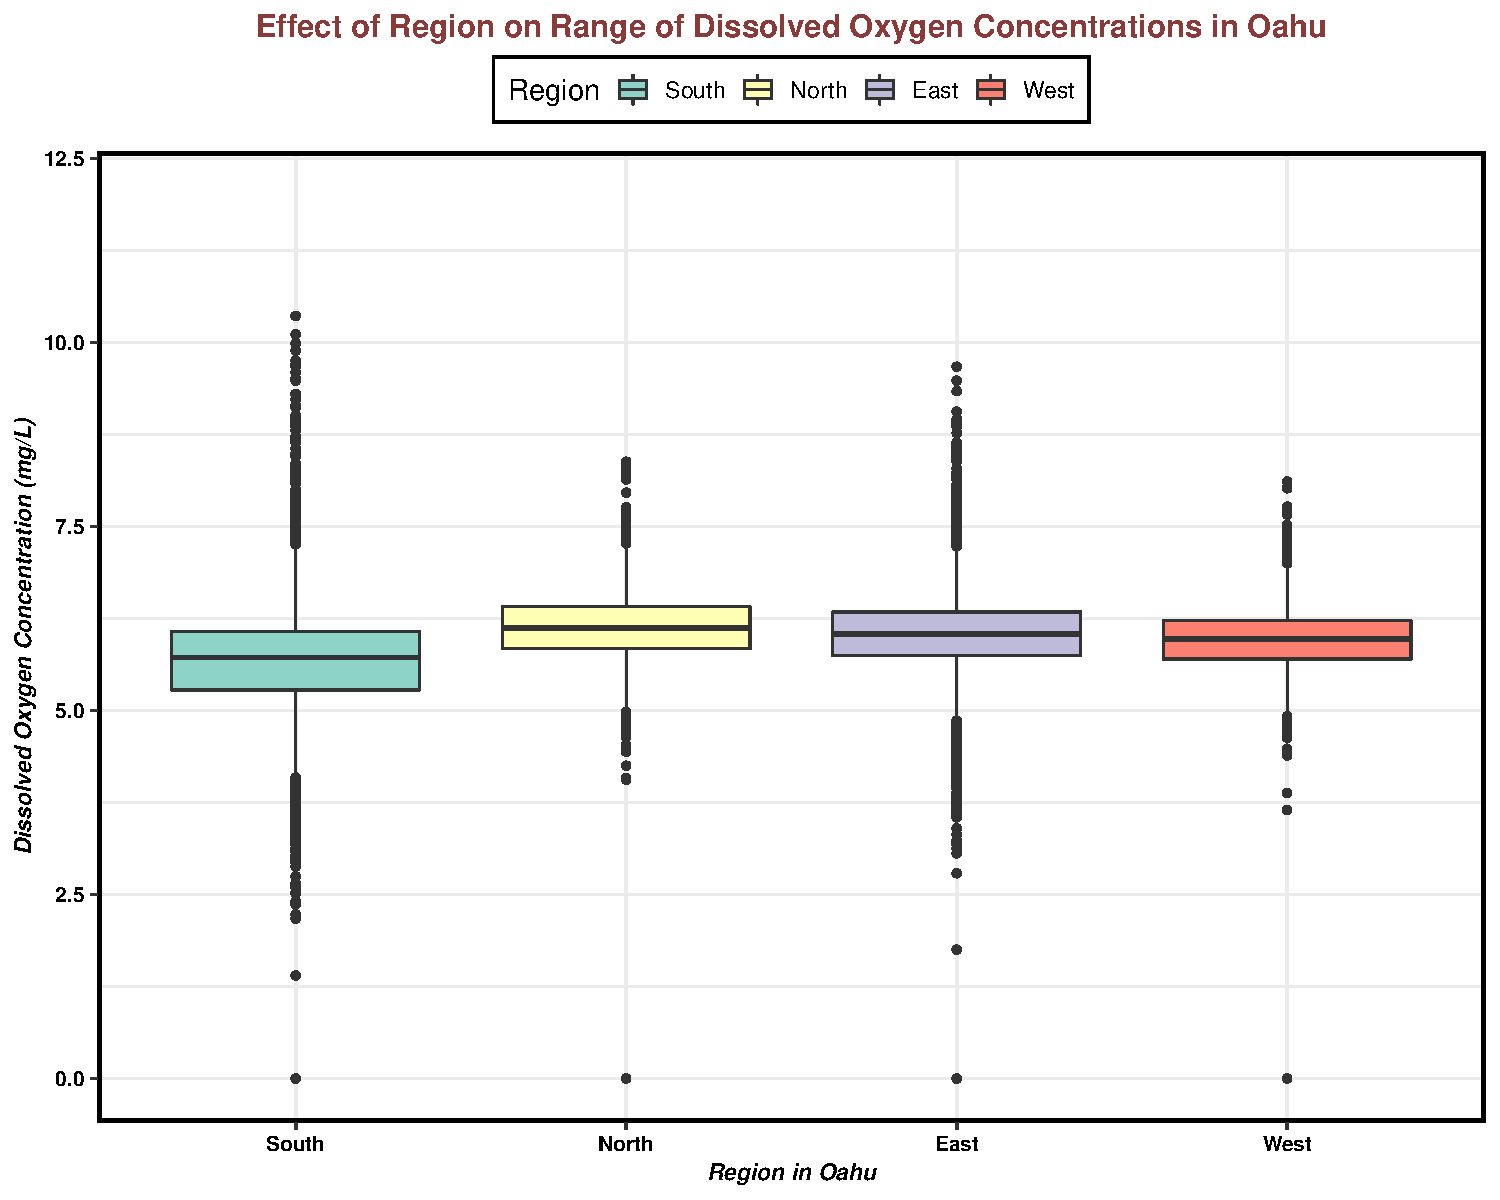
\includegraphics{Garcia_ENV872_Project_files/figure-latex/unnamed-chunk-56-1.pdf}

\newpage

\section{Statistical Analysis}\label{statistical-analysis}

\subsection{Full Maximal Model}\label{full-maximal-model}

\begin{Shaded}
\begin{Highlighting}[]
\KeywordTok{attach}\NormalTok{(OahuDataClean)}
\NormalTok{HawaiiModClean<-}\KeywordTok{lm}\NormalTok{(DO}\OperatorTok{~}\NormalTok{Enterococcus }\OperatorTok{+}\StringTok{ }\NormalTok{Temperature }\OperatorTok{+}\NormalTok{Salinity }\OperatorTok{+}\NormalTok{pH }\OperatorTok{+}\StringTok{ }\NormalTok{Turbidity }\OperatorTok{+}\StringTok{ }\NormalTok{CP.Result, }\DataTypeTok{data=}\NormalTok{OahuDataClean)}
\KeywordTok{summary}\NormalTok{(HawaiiModClean)}
\end{Highlighting}
\end{Shaded}

\begin{verbatim}
## 
## Call:
## lm(formula = DO ~ Enterococcus + Temperature + Salinity + pH + 
##     Turbidity + CP.Result, data = OahuDataClean)
## 
## Residuals:
##     Min      1Q  Median      3Q     Max 
## -11.649  -0.275   0.125   0.467  85.579 
## 
## Coefficients:
##                Estimate Std. Error t value Pr(>|t|)    
## (Intercept)   2.430e+00  1.262e-01  19.253  < 2e-16 ***
## Enterococcus  1.108e-04  4.419e-05   2.507   0.0122 *  
## Temperature   1.946e-02  4.737e-03   4.108 4.01e-05 ***
## Salinity      4.203e-02  3.205e-03  13.112  < 2e-16 ***
## pH            1.709e-01  8.990e-03  19.008  < 2e-16 ***
## Turbidity    -2.084e-03  1.134e-03  -1.837   0.0662 .  
## CP.Result    -1.602e-04  1.182e-03  -0.136   0.8922    
## ---
## Signif. codes:  0 '***' 0.001 '**' 0.01 '*' 0.05 '.' 0.1 ' ' 1
## 
## Residual standard error: 1.312 on 22903 degrees of freedom
## Multiple R-squared:  0.0397, Adjusted R-squared:  0.03944 
## F-statistic: 157.8 on 6 and 22903 DF,  p-value: < 2.2e-16
\end{verbatim}

\subsection{Remove Specific Heat
Parameter}\label{remove-specific-heat-parameter}

\begin{Shaded}
\begin{Highlighting}[]
\NormalTok{HawaiiModClean2<-}\KeywordTok{update}\NormalTok{(HawaiiModClean,.}\OperatorTok{~}\NormalTok{.}\OperatorTok{-}\NormalTok{CP.Result)}
\KeywordTok{summary}\NormalTok{(HawaiiModClean2)}
\end{Highlighting}
\end{Shaded}

\begin{verbatim}
## 
## Call:
## lm(formula = DO ~ Enterococcus + Temperature + Salinity + pH + 
##     Turbidity, data = OahuDataClean)
## 
## Residuals:
##     Min      1Q  Median      3Q     Max 
## -11.648  -0.275   0.125   0.467  85.579 
## 
## Coefficients:
##                Estimate Std. Error t value Pr(>|t|)    
## (Intercept)   2.430e+00  1.261e-01  19.262  < 2e-16 ***
## Enterococcus  1.087e-04  4.145e-05   2.623  0.00873 ** 
## Temperature   1.946e-02  4.737e-03   4.108    4e-05 ***
## Salinity      4.204e-02  3.203e-03  13.124  < 2e-16 ***
## pH            1.709e-01  8.989e-03  19.008  < 2e-16 ***
## Turbidity    -2.116e-03  1.110e-03  -1.906  0.05667 .  
## ---
## Signif. codes:  0 '***' 0.001 '**' 0.01 '*' 0.05 '.' 0.1 ' ' 1
## 
## Residual standard error: 1.312 on 22904 degrees of freedom
## Multiple R-squared:  0.03969,    Adjusted R-squared:  0.03948 
## F-statistic: 189.3 on 5 and 22904 DF,  p-value: < 2.2e-16
\end{verbatim}

\subsection{Remove Turbidity
Parameter}\label{remove-turbidity-parameter}

\begin{Shaded}
\begin{Highlighting}[]
\NormalTok{HawaiiModClean3<-}\KeywordTok{update}\NormalTok{(HawaiiModClean2,.}\OperatorTok{~}\NormalTok{.}\OperatorTok{-}\NormalTok{Turbidity)}
\KeywordTok{summary}\NormalTok{(HawaiiModClean3)}
\end{Highlighting}
\end{Shaded}

\begin{verbatim}
## 
## Call:
## lm(formula = DO ~ Enterococcus + Temperature + Salinity + pH, 
##     data = OahuDataClean)
## 
## Residuals:
##     Min      1Q  Median      3Q     Max 
## -11.639  -0.277   0.125   0.467  85.585 
## 
## Coefficients:
##               Estimate Std. Error t value Pr(>|t|)    
## (Intercept)  2.407e+00  1.256e-01  19.167  < 2e-16 ***
## Enterococcus 1.001e-04  4.121e-05   2.430   0.0151 *  
## Temperature  1.960e-02  4.737e-03   4.137 3.53e-05 ***
## Salinity     4.226e-02  3.201e-03  13.202  < 2e-16 ***
## pH           1.709e-01  8.990e-03  19.006  < 2e-16 ***
## ---
## Signif. codes:  0 '***' 0.001 '**' 0.01 '*' 0.05 '.' 0.1 ' ' 1
## 
## Residual standard error: 1.312 on 22905 degrees of freedom
## Multiple R-squared:  0.03954,    Adjusted R-squared:  0.03937 
## F-statistic: 235.7 on 4 and 22905 DF,  p-value: < 2.2e-16
\end{verbatim}

\subsection{AIC Test of all models}\label{aic-test-of-all-models}

\begin{Shaded}
\begin{Highlighting}[]
\KeywordTok{AIC}\NormalTok{(HawaiiModClean, HawaiiModClean2, HawaiiModClean3)}
\end{Highlighting}
\end{Shaded}

\begin{verbatim}
##                 df      AIC
## HawaiiModClean   8 77462.89
## HawaiiModClean2  7 77460.91
## HawaiiModClean3  6 77462.54
\end{verbatim}

\subsection{Partial F-test of all
Models}\label{partial-f-test-of-all-models}

\begin{Shaded}
\begin{Highlighting}[]
\KeywordTok{anova}\NormalTok{(HawaiiModClean, HawaiiModClean2, HawaiiModClean3)}
\end{Highlighting}
\end{Shaded}

\begin{verbatim}
## Analysis of Variance Table
## 
## Model 1: DO ~ Enterococcus + Temperature + Salinity + pH + Turbidity + 
##     CP.Result
## Model 2: DO ~ Enterococcus + Temperature + Salinity + pH + Turbidity
## Model 3: DO ~ Enterococcus + Temperature + Salinity + pH
##   Res.Df   RSS Df Sum of Sq      F  Pr(>F)  
## 1  22903 39416                              
## 2  22904 39416 -1   -0.0316 0.0184 0.89216  
## 3  22905 39423 -1   -6.2513 3.6324 0.05668 .
## ---
## Signif. codes:  0 '***' 0.001 '**' 0.01 '*' 0.05 '.' 0.1 ' ' 1
\end{verbatim}

\subsection{Check for Multicollinearity of Final
Model}\label{check-for-multicollinearity-of-final-model}

\begin{Shaded}
\begin{Highlighting}[]
\KeywordTok{vif}\NormalTok{(HawaiiModClean3)}
\end{Highlighting}
\end{Shaded}

\begin{verbatim}
## Enterococcus  Temperature     Salinity           pH 
##     1.012229     1.232857     1.279092     1.134850
\end{verbatim}

\subsubsection{Check Residuals of
HawaiiModClean3}\label{check-residuals-of-hawaiimodclean3}

\begin{Shaded}
\begin{Highlighting}[]
\KeywordTok{par}\NormalTok{(}\DataTypeTok{mfrow=}\KeywordTok{c}\NormalTok{(}\DecValTok{2}\NormalTok{,}\DecValTok{2}\NormalTok{))}
\KeywordTok{plot}\NormalTok{(HawaiiModClean3)}
\end{Highlighting}
\end{Shaded}

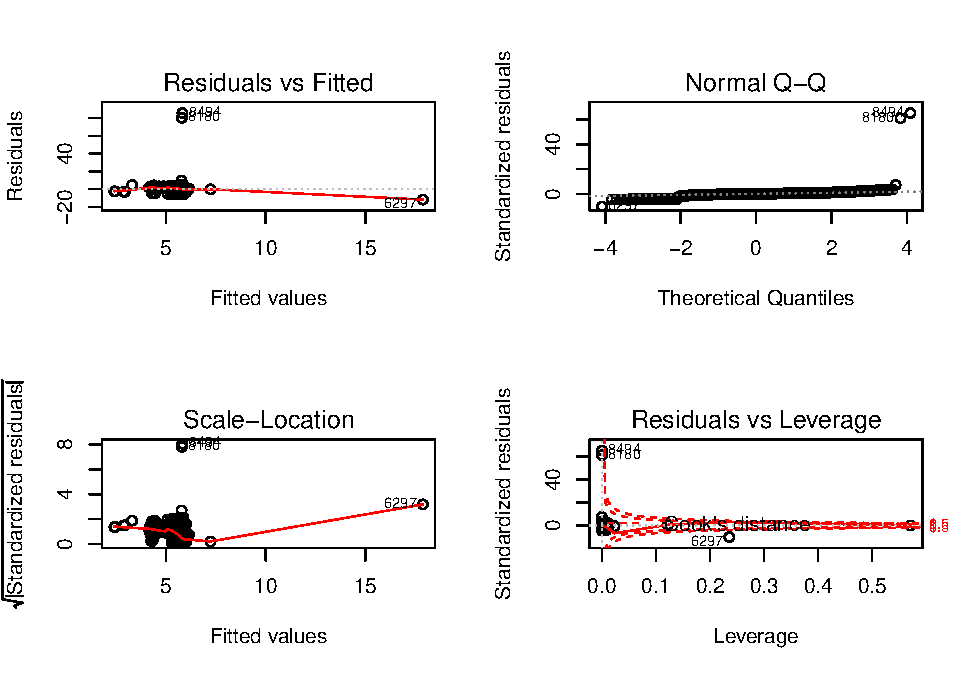
\includegraphics{Garcia_ENV872_Project_files/figure-latex/unnamed-chunk-63-1.pdf}

\section{Research question: Is there a trend over time in DO
concentrations by region in
Oahu?}\label{research-question-is-there-a-trend-over-time-in-do-concentrations-by-region-in-oahu}

\subsubsection{Split Dataset by Region (Use full
dataset)}\label{split-dataset-by-region-use-full-dataset}

\begin{Shaded}
\begin{Highlighting}[]
\NormalTok{HawaiiWaterCleanOahuNorth<-}\StringTok{ }\KeywordTok{filter}\NormalTok{(OahuDataClean, Region}\OperatorTok{==}\StringTok{ "North"}\NormalTok{)}
\NormalTok{HawaiiWaterCleanOahuSouth<-}\StringTok{ }\KeywordTok{filter}\NormalTok{(OahuDataClean, Region}\OperatorTok{==}\StringTok{ "South"}\NormalTok{)}
\NormalTok{HawaiiWaterCleanOahuEast<-}\StringTok{ }\KeywordTok{filter}\NormalTok{(OahuDataClean, Region}\OperatorTok{==}\StringTok{ "East"}\NormalTok{)}
\NormalTok{HawaiiWaterCleanOahuWest<-}\StringTok{ }\KeywordTok{filter}\NormalTok{(OahuDataClean, Region}\OperatorTok{==}\StringTok{ "West"}\NormalTok{)}
\end{Highlighting}
\end{Shaded}

\subsection{Run a Mann Kendall Test for North
Oahu}\label{run-a-mann-kendall-test-for-north-oahu}

\begin{Shaded}
\begin{Highlighting}[]
\KeywordTok{library}\NormalTok{(trend)}
\KeywordTok{mk.test}\NormalTok{(HawaiiWaterCleanOahuNorth}\OperatorTok{$}\NormalTok{DO)}
\end{Highlighting}
\end{Shaded}

\begin{verbatim}
## 
##  Mann-Kendall trend test
## 
## data:  HawaiiWaterCleanOahuNorth$DO
## z = -21.099, n = 2638, p-value < 2.2e-16
## alternative hypothesis: true S is not equal to 0
## sample estimates:
##             S          varS           tau 
## -9.531430e+05  2.040778e+09 -2.749711e-01
\end{verbatim}

\subsection{Run a Mann Kendall Test for South
Oahu}\label{run-a-mann-kendall-test-for-south-oahu}

\begin{Shaded}
\begin{Highlighting}[]
\KeywordTok{library}\NormalTok{(trend)}
\KeywordTok{mk.test}\NormalTok{(HawaiiWaterCleanOahuSouth}\OperatorTok{$}\NormalTok{DO)}
\end{Highlighting}
\end{Shaded}

\begin{verbatim}
## 
##  Mann-Kendall trend test
## 
## data:  HawaiiWaterCleanOahuSouth$DO
## z = -28.432, n = 12262, p-value < 2.2e-16
## alternative hypothesis: true S is not equal to 0
## sample estimates:
##             S          varS           tau 
## -1.286915e+07  2.048692e+11 -1.716364e-01
\end{verbatim}

\subsection{Run a Mann Kendall Test for East
Oahu}\label{run-a-mann-kendall-test-for-east-oahu}

\begin{Shaded}
\begin{Highlighting}[]
\KeywordTok{library}\NormalTok{(trend)}
\KeywordTok{mk.test}\NormalTok{(HawaiiWaterCleanOahuEast}\OperatorTok{$}\NormalTok{DO)}
\end{Highlighting}
\end{Shaded}

\begin{verbatim}
## 
##  Mann-Kendall trend test
## 
## data:  HawaiiWaterCleanOahuEast$DO
## z = -19.186, n = 4694, p-value < 2.2e-16
## alternative hypothesis: true S is not equal to 0
## sample estimates:
##             S          varS           tau 
## -2.056955e+06  1.149472e+10 -1.873351e-01
\end{verbatim}

\subsection{Run a Mann Kendall Test for West
Oahu}\label{run-a-mann-kendall-test-for-west-oahu}

\begin{Shaded}
\begin{Highlighting}[]
\KeywordTok{library}\NormalTok{(trend)}
\KeywordTok{mk.test}\NormalTok{(HawaiiWaterCleanOahuWest}\OperatorTok{$}\NormalTok{DO)}
\end{Highlighting}
\end{Shaded}

\begin{verbatim}
## 
##  Mann-Kendall trend test
## 
## data:  HawaiiWaterCleanOahuWest$DO
## z = -21.833, n = 3316, p-value < 2.2e-16
## alternative hypothesis: true S is not equal to 0
## sample estimates:
##             S          varS           tau 
## -1.389943e+06  4.052891e+09 -2.538011e-01
\end{verbatim}

For North Oahu, the z-value is 17.91, so we see a negative trend in DO
concentrations over time. The p-value is \textless{} 2.2e-16,so we
reject the null hypothesis that the data come from a population with
independent realizations and are identically distributed . For South
Oahu, the z-value is -28.477, so we see a negative trend in DO
concentrations over time. The p-value for South Oahu is listed as
9.14e-13, so we reject the null hypothesis that the data come from a
population with independent realizations and are identically
distributed. For East Oahu, the z-value is -23.022, and p-value is
\textless{} 2.2e-16, so we reject the null hypothesis that the data come
from a population with independent realizations and are identically
distributed; there is a negative trend in DO concentrations over time.
For West Oahu, the z-value is -21.849, so there is also a negative trend
in DO concentrations over time.

\section{North Oahu}\label{north-oahu}

\subsubsection{Arrange North Oahu Dataset by Date
(ascending)}\label{arrange-north-oahu-dataset-by-date-ascending}

\begin{Shaded}
\begin{Highlighting}[]
\NormalTok{HawaiiWaterCleanOahuNorth<-}\KeywordTok{arrange}\NormalTok{(HawaiiWaterCleanOahuNorth, Date)}
\end{Highlighting}
\end{Shaded}

\subsection{Pettit's Test for North
Oahu}\label{pettits-test-for-north-oahu}

\begin{Shaded}
\begin{Highlighting}[]
\KeywordTok{pettitt.test}\NormalTok{(HawaiiWaterCleanOahuNorth}\OperatorTok{$}\NormalTok{DO)}
\end{Highlighting}
\end{Shaded}

\begin{verbatim}
## 
##  Pettitt's test for single change-point detection
## 
## data:  HawaiiWaterCleanOahuNorth$DO
## U* = 508840, p-value < 2.2e-16
## alternative hypothesis: two.sided
## sample estimates:
## probable change point at time K 
##                            1716
\end{verbatim}

Because the p-value is \textless{}0.05, the change point is significant.
Given 1st change point for North Oahu is 1332, we scroll to observation
1332 in data set, so first change point occurred in 2009-01-12.

\subsection{Run a separate Mann-Kendall Test for Each Change
Point}\label{run-a-separate-mann-kendall-test-for-each-change-point}

\begin{Shaded}
\begin{Highlighting}[]
\KeywordTok{mk.test}\NormalTok{(HawaiiWaterCleanOahuNorth}\OperatorTok{$}\NormalTok{DO[}\DecValTok{1}\OperatorTok{:}\DecValTok{1331}\NormalTok{])}
\end{Highlighting}
\end{Shaded}

\begin{verbatim}
## 
##  Mann-Kendall trend test
## 
## data:  HawaiiWaterCleanOahuNorth$DO[1:1331]
## z = 10.561, n = 1331, p-value < 2.2e-16
## alternative hypothesis: true S is not equal to 0
## sample estimates:
##            S         varS          tau 
## 1.710250e+05 2.622598e+08 1.939526e-01
\end{verbatim}

\begin{Shaded}
\begin{Highlighting}[]
\KeywordTok{mk.test}\NormalTok{(HawaiiWaterCleanOahuNorth}\OperatorTok{$}\NormalTok{DO[}\DecValTok{1332}\OperatorTok{:}\DecValTok{2638}\NormalTok{])}
\end{Highlighting}
\end{Shaded}

\begin{verbatim}
## 
##  Mann-Kendall trend test
## 
## data:  HawaiiWaterCleanOahuNorth$DO[1332:2638]
## z = -11.825, n = 1307, p-value < 2.2e-16
## alternative hypothesis: true S is not equal to 0
## sample estimates:
##             S          varS           tau 
## -1.863460e+05  2.483412e+08 -2.190577e-01
\end{verbatim}

Second change point p-value\textless{}0.05, so there is a significant
second change point.

\section{What is the second change
point?}\label{what-is-the-second-change-point}

\begin{Shaded}
\begin{Highlighting}[]
\KeywordTok{pettitt.test}\NormalTok{(HawaiiWaterCleanOahuNorth}\OperatorTok{$}\NormalTok{DO[}\DecValTok{1332}\OperatorTok{:}\DecValTok{2638}\NormalTok{])  }
\end{Highlighting}
\end{Shaded}

\begin{verbatim}
## 
##  Pettitt's test for single change-point detection
## 
## data:  HawaiiWaterCleanOahuNorth$DO[1332:2638]
## U* = 157400, p-value < 2.2e-16
## alternative hypothesis: two.sided
## sample estimates:
## probable change point at time K 
##                             531
\end{verbatim}

1332 + 942=2274, so look at 2274 row in datatable to see second change
point. It happened on 2017-10-19.

\section{Check for a third change
point}\label{check-for-a-third-change-point}

\paragraph{Now split dataset into three
pieces}\label{now-split-dataset-into-three-pieces}

\begin{Shaded}
\begin{Highlighting}[]
\KeywordTok{mk.test}\NormalTok{(HawaiiWaterCleanOahuNorth}\OperatorTok{$}\NormalTok{DO[}\DecValTok{1332}\OperatorTok{:}\DecValTok{2273}\NormalTok{])  }
\end{Highlighting}
\end{Shaded}

\begin{verbatim}
## 
##  Mann-Kendall trend test
## 
## data:  HawaiiWaterCleanOahuNorth$DO[1332:2273]
## z = -11.017, n = 942, p-value < 2.2e-16
## alternative hypothesis: true S is not equal to 0
## sample estimates:
##             S          varS           tau 
## -1.062570e+05  9.301715e+07 -2.405171e-01
\end{verbatim}

\begin{Shaded}
\begin{Highlighting}[]
\KeywordTok{mk.test}\NormalTok{(HawaiiWaterCleanOahuNorth}\OperatorTok{$}\NormalTok{DO[}\DecValTok{2274}\OperatorTok{:}\DecValTok{2638}\NormalTok{])  }
\end{Highlighting}
\end{Shaded}

\begin{verbatim}
## 
##  Mann-Kendall trend test
## 
## data:  HawaiiWaterCleanOahuNorth$DO[2274:2638]
## z = -0.60241, n = 365, p-value = 0.5469
## alternative hypothesis: true S is not equal to 0
## sample estimates:
##             S          varS           tau 
## -1.404000e+03  5.424163e+06 -2.122081e-02
\end{verbatim}

If z-score is positive, it's a positive trend in DO concentrations over
time. If z-score is negative, it is a negative trend in DO
concentrations over time. There is a significant trend for
rows:2856:3271 because the p-value is below 0.05, so there is a third
changepoint.

\section{What is third change point?}\label{what-is-third-change-point}

\begin{Shaded}
\begin{Highlighting}[]
\KeywordTok{pettitt.test}\NormalTok{(HawaiiWaterCleanOahuNorth}\OperatorTok{$}\NormalTok{DO[}\DecValTok{2274}\OperatorTok{:}\DecValTok{2638}\NormalTok{])  }
\end{Highlighting}
\end{Shaded}

\begin{verbatim}
## 
##  Pettitt's test for single change-point detection
## 
## data:  HawaiiWaterCleanOahuNorth$DO[2274:2638]
## U* = 3555, p-value = 0.4223
## alternative hypothesis: two.sided
## sample estimates:
## probable change point at time K 
##                             115
\end{verbatim}

2274+215=2489--\textgreater{}Third change point happened on 2018-11-29

\subsubsection{Change Date to be a date
object}\label{change-date-to-be-a-date-object}

\begin{Shaded}
\begin{Highlighting}[]
\NormalTok{HawaiiWaterCleanOahuNorth}\OperatorTok{$}\NormalTok{Date<-}\KeywordTok{as.Date}\NormalTok{(HawaiiWaterCleanOahuNorth}\OperatorTok{$}\NormalTok{Date, }\DataTypeTok{format =} \StringTok{"%m/%d/%y"}\NormalTok{)}
\end{Highlighting}
\end{Shaded}

\section{Time Series of DO Concentrations in North Oahu with
Changepoints}\label{time-series-of-do-concentrations-in-north-oahu-with-changepoints}

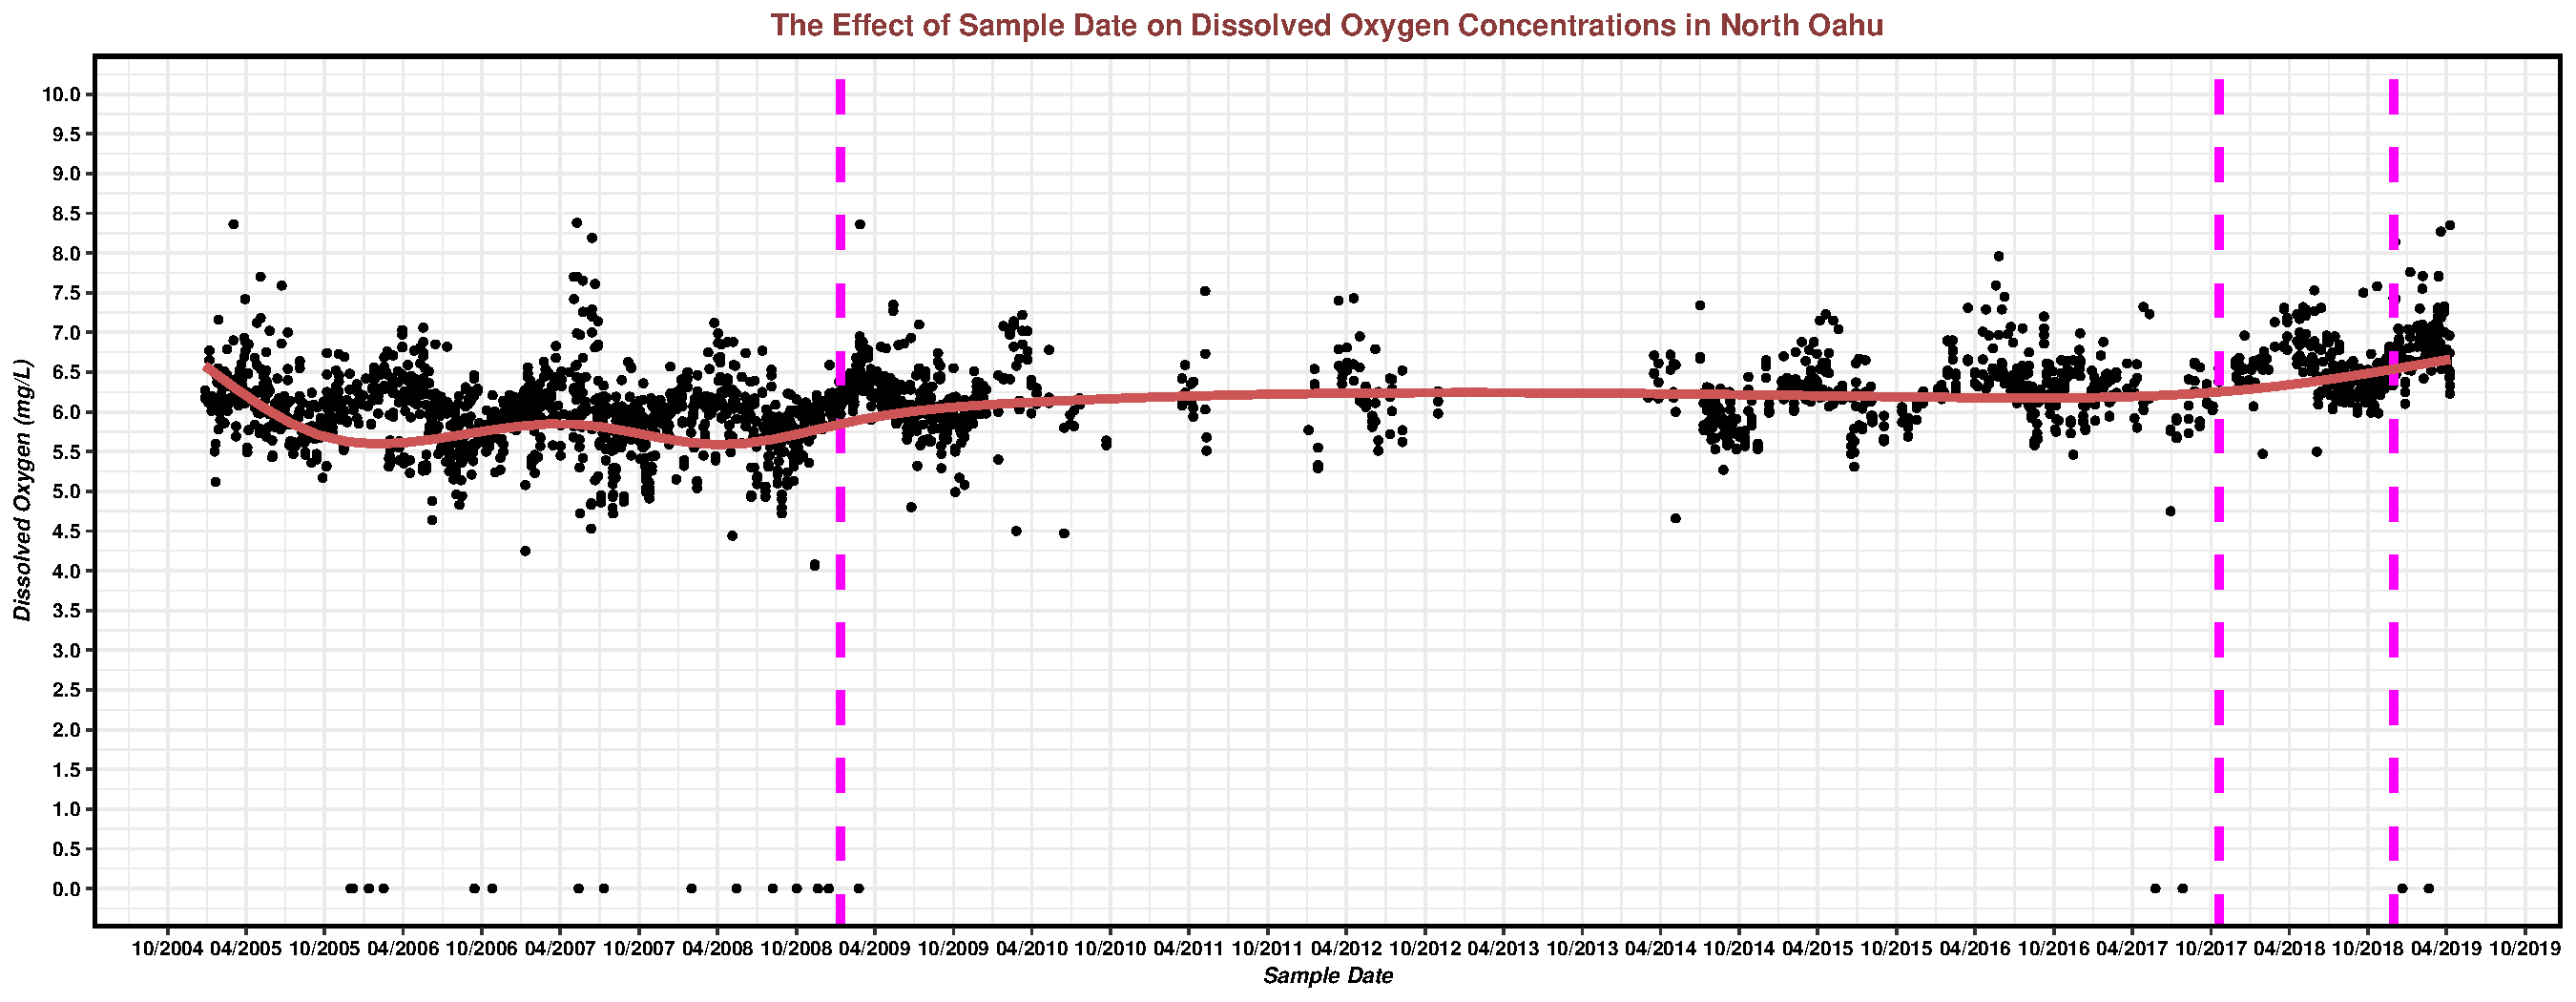
\includegraphics{Garcia_ENV872_Project_files/figure-latex/North Oahu-1.pdf}

\section{South Oahu}\label{south-oahu}

\subsubsection{Change Date to be a date
object}\label{change-date-to-be-a-date-object-1}

\begin{Shaded}
\begin{Highlighting}[]
\NormalTok{HawaiiWaterCleanOahuSouth}\OperatorTok{$}\NormalTok{Date<-}\KeywordTok{as.Date}\NormalTok{(HawaiiWaterCleanOahuSouth}\OperatorTok{$}\NormalTok{Date, }\DataTypeTok{format =} \StringTok{"%m/%d/%y"}\NormalTok{)}
\end{Highlighting}
\end{Shaded}

\subsubsection{Arrange South Oahu Dataset by Date
(ascending)}\label{arrange-south-oahu-dataset-by-date-ascending}

\begin{Shaded}
\begin{Highlighting}[]
\NormalTok{HawaiiWaterCleanOahuSouth<-dplyr}\OperatorTok{::}\KeywordTok{arrange}\NormalTok{(HawaiiWaterCleanOahuSouth, Date)}
\end{Highlighting}
\end{Shaded}

\subsection{Pettit's Test for South
Oahu}\label{pettits-test-for-south-oahu}

\begin{Shaded}
\begin{Highlighting}[]
\KeywordTok{pettitt.test}\NormalTok{(HawaiiWaterCleanOahuSouth}\OperatorTok{$}\NormalTok{DO)}
\end{Highlighting}
\end{Shaded}

\begin{verbatim}
## 
##  Pettitt's test for single change-point detection
## 
## data:  HawaiiWaterCleanOahuSouth$DO
## U* = 12103000, p-value < 2.2e-16
## alternative hypothesis: two.sided
## sample estimates:
## probable change point at time K 
##                            9303
\end{verbatim}

Because the p-value is \textless{}0.05, the change point is significant.
Given 1st change point for South Oahu is 9303, we scroll to observation
9303 in data set, so first change point occurred in 2012-12-12

\subsection{Run a separate Mann-Kendall Test for Each Change
Point}\label{run-a-separate-mann-kendall-test-for-each-change-point-1}

\begin{Shaded}
\begin{Highlighting}[]
\KeywordTok{mk.test}\NormalTok{(HawaiiWaterCleanOahuSouth}\OperatorTok{$}\NormalTok{DO[}\DecValTok{1}\OperatorTok{:}\DecValTok{9302}\NormalTok{])}
\end{Highlighting}
\end{Shaded}

\begin{verbatim}
## 
##  Mann-Kendall trend test
## 
## data:  HawaiiWaterCleanOahuSouth$DO[1:9302]
## z = -2.1972, n = 9302, p-value = 0.02801
## alternative hypothesis: true S is not equal to 0
## sample estimates:
##             S          varS           tau 
## -6.571130e+05  8.944082e+10 -1.523163e-02
\end{verbatim}

\begin{Shaded}
\begin{Highlighting}[]
\KeywordTok{mk.test}\NormalTok{(HawaiiWaterCleanOahuSouth}\OperatorTok{$}\NormalTok{DO[}\DecValTok{9303}\OperatorTok{:}\DecValTok{12262}\NormalTok{])}
\end{Highlighting}
\end{Shaded}

\begin{verbatim}
## 
##  Mann-Kendall trend test
## 
## data:  HawaiiWaterCleanOahuSouth$DO[9303:12262]
## z = 26.793, n = 2960, p-value < 2.2e-16
## alternative hypothesis: true S is not equal to 0
## sample estimates:
##            S         varS          tau 
## 1.438590e+06 2.882930e+09 3.293585e-01
\end{verbatim}

p-value for {[}9303:12262{]} is significant, so run a Pettit's Test for
second change point

\subsection{What is second change
point?}\label{what-is-second-change-point}

\begin{Shaded}
\begin{Highlighting}[]
\KeywordTok{pettitt.test}\NormalTok{(HawaiiWaterCleanOahuSouth}\OperatorTok{$}\NormalTok{DO[}\DecValTok{9303}\OperatorTok{:}\DecValTok{12262}\NormalTok{])}
\end{Highlighting}
\end{Shaded}

\begin{verbatim}
## 
##  Pettitt's test for single change-point detection
## 
## data:  HawaiiWaterCleanOahuSouth$DO[9303:12262]
## U* = 1287300, p-value < 2.2e-16
## alternative hypothesis: two.sided
## sample estimates:
## probable change point at time K 
##                            1922
\end{verbatim}

9303 + 1922=11235, scroll to observation 11225 in data set, so second
change point occurred in 2017-11-28

\subsection{Run another Mann-Kendall to check for second change
point}\label{run-another-mann-kendall-to-check-for-second-change-point}

\paragraph{Now split dataset into three
pieces}\label{now-split-dataset-into-three-pieces-1}

\begin{Shaded}
\begin{Highlighting}[]
\KeywordTok{mk.test}\NormalTok{(HawaiiWaterCleanOahuSouth}\OperatorTok{$}\NormalTok{DO[}\DecValTok{9303}\OperatorTok{:}\DecValTok{11224}\NormalTok{])   }
\end{Highlighting}
\end{Shaded}

\begin{verbatim}
## 
##  Mann-Kendall trend test
## 
## data:  HawaiiWaterCleanOahuSouth$DO[9303:11224]
## z = 3.5054, n = 1922, p-value = 0.000456
## alternative hypothesis: true S is not equal to 0
## sample estimates:
##            S         varS          tau 
## 9.849200e+04 7.894562e+08 5.352165e-02
\end{verbatim}

\begin{Shaded}
\begin{Highlighting}[]
\KeywordTok{mk.test}\NormalTok{(HawaiiWaterCleanOahuSouth}\OperatorTok{$}\NormalTok{DO[}\DecValTok{11225}\OperatorTok{:}\DecValTok{12262}\NormalTok{])  }
\end{Highlighting}
\end{Shaded}

\begin{verbatim}
## 
##  Mann-Kendall trend test
## 
## data:  HawaiiWaterCleanOahuSouth$DO[11225:12262]
## z = 4.7353, n = 1038, p-value = 2.187e-06
## alternative hypothesis: true S is not equal to 0
## sample estimates:
##            S         varS          tau 
## 5.282400e+04 1.244360e+08 9.844092e-02
\end{verbatim}

Because p\textless{}0.05, there is a significant change point in rows
{[}11225:12262{]}

\subsection{Third Change Point}\label{third-change-point}

\begin{Shaded}
\begin{Highlighting}[]
\KeywordTok{pettitt.test}\NormalTok{(HawaiiWaterCleanOahuSouth}\OperatorTok{$}\NormalTok{DO[}\DecValTok{11225}\OperatorTok{:}\DecValTok{12262}\NormalTok{])}
\end{Highlighting}
\end{Shaded}

\begin{verbatim}
## 
##  Pettitt's test for single change-point detection
## 
## data:  HawaiiWaterCleanOahuSouth$DO[11225:12262]
## U* = 81125, p-value = 9.591e-16
## alternative hypothesis: two.sided
## sample estimates:
## probable change point at time K 
##                             692
\end{verbatim}

11225+ 692=11917--\textgreater{}third change point occurred 2018-12-04

\section{Time Series of DO Concentrations in South Oahu with
Changepoints}\label{time-series-of-do-concentrations-in-south-oahu-with-changepoints}

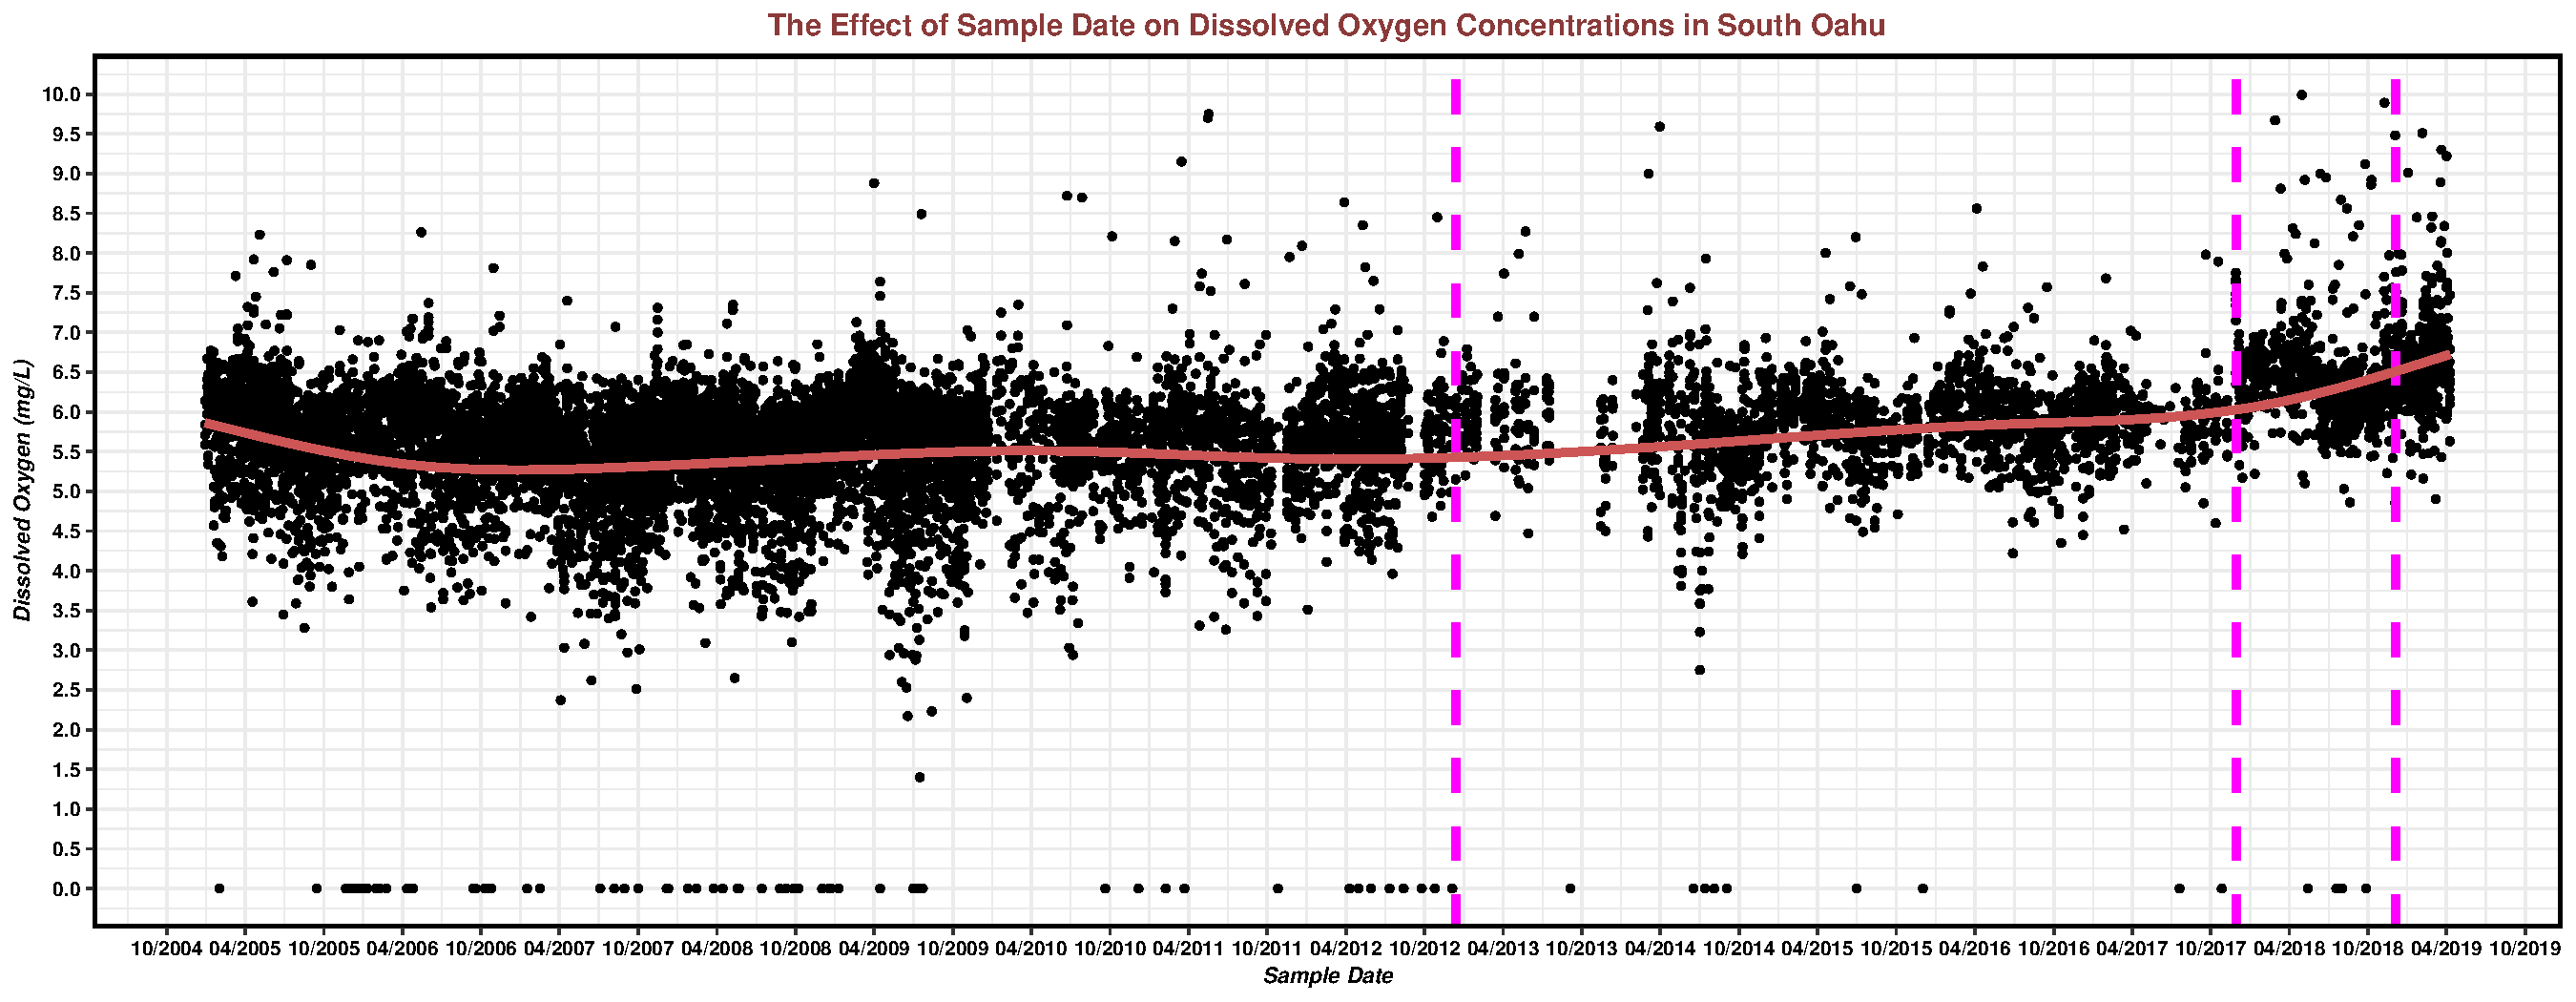
\includegraphics{Garcia_ENV872_Project_files/figure-latex/South Oahu-1.pdf}

\section{West Oahu}\label{west-oahu}

\subsubsection{Change Date to be a date
object}\label{change-date-to-be-a-date-object-2}

\begin{Shaded}
\begin{Highlighting}[]
\NormalTok{HawaiiWaterCleanOahuWest}\OperatorTok{$}\NormalTok{Date<-}\KeywordTok{as.Date}\NormalTok{(HawaiiWaterCleanOahuWest}\OperatorTok{$}\NormalTok{Date, }\DataTypeTok{format =} \StringTok{"%m/%d/%y"}\NormalTok{)}
\end{Highlighting}
\end{Shaded}

\subsubsection{Arrange West Oahu Dataset by Date
(ascending)}\label{arrange-west-oahu-dataset-by-date-ascending}

\begin{Shaded}
\begin{Highlighting}[]
\NormalTok{HawaiiWaterCleanOahuWest<-dplyr}\OperatorTok{::}\KeywordTok{arrange}\NormalTok{(HawaiiWaterCleanOahuWest, Date)}
\end{Highlighting}
\end{Shaded}

\subsection{Pettit's Test for West
Oahu}\label{pettits-test-for-west-oahu}

\begin{Shaded}
\begin{Highlighting}[]
\KeywordTok{pettitt.test}\NormalTok{(HawaiiWaterCleanOahuWest}\OperatorTok{$}\NormalTok{DO)}
\end{Highlighting}
\end{Shaded}

\begin{verbatim}
## 
##  Pettitt's test for single change-point detection
## 
## data:  HawaiiWaterCleanOahuWest$DO
## U* = 1180500, p-value < 2.2e-16
## alternative hypothesis: two.sided
## sample estimates:
## probable change point at time K 
##                            1752
\end{verbatim}

Because the p-value is \textless{}0.05, the change point is significant.
Given 1st change point for West Oahu is 1752, we scroll to observation
1752 in data set, so first change point occurred in 2009-01-20

\subsection{Run a separate Mann-Kendall Test for Each Change
Point}\label{run-a-separate-mann-kendall-test-for-each-change-point-2}

\begin{Shaded}
\begin{Highlighting}[]
\KeywordTok{mk.test}\NormalTok{(HawaiiWaterCleanOahuWest}\OperatorTok{$}\NormalTok{DO[}\DecValTok{1}\OperatorTok{:}\DecValTok{1751}\NormalTok{])}
\end{Highlighting}
\end{Shaded}

\begin{verbatim}
## 
##  Mann-Kendall trend test
## 
## data:  HawaiiWaterCleanOahuWest$DO[1:1751]
## z = -5.4424, n = 1751, p-value = 5.258e-08
## alternative hypothesis: true S is not equal to 0
## sample estimates:
##             S          varS           tau 
## -1.329730e+05  5.969618e+08 -8.712235e-02
\end{verbatim}

\begin{Shaded}
\begin{Highlighting}[]
\KeywordTok{mk.test}\NormalTok{(HawaiiWaterCleanOahuWest}\OperatorTok{$}\NormalTok{DO[}\DecValTok{1752}\OperatorTok{:}\DecValTok{3316}\NormalTok{])}
\end{Highlighting}
\end{Shaded}

\begin{verbatim}
## 
##  Mann-Kendall trend test
## 
## data:  HawaiiWaterCleanOahuWest$DO[1752:3316]
## z = 16.683, n = 1565, p-value < 2.2e-16
## alternative hypothesis: true S is not equal to 0
## sample estimates:
##            S         varS          tau 
## 3.444320e+05 4.262618e+08 2.825216e-01
\end{verbatim}

p-value for {[}1752:3316{]} is significant, so run a Pettit's Test for
second change point

\subsection{What is second change
point?}\label{what-is-second-change-point-1}

\begin{Shaded}
\begin{Highlighting}[]
\KeywordTok{pettitt.test}\NormalTok{(HawaiiWaterCleanOahuWest}\OperatorTok{$}\NormalTok{DO[}\DecValTok{1752}\OperatorTok{:}\DecValTok{3316}\NormalTok{])}
\end{Highlighting}
\end{Shaded}

\begin{verbatim}
## 
##  Pettitt's test for single change-point detection
## 
## data:  HawaiiWaterCleanOahuWest$DO[1752:3316]
## U* = 318050, p-value < 2.2e-16
## alternative hypothesis: two.sided
## sample estimates:
## probable change point at time K 
##                            1118
\end{verbatim}

1752+ 1118=2870, scroll to observation 2870 in data set, so second
change point occurred in 2017-11-29

\subsection{Run another Mann-Kendall to check for third change
point}\label{run-another-mann-kendall-to-check-for-third-change-point}

\paragraph{Now split dataset into three
pieces}\label{now-split-dataset-into-three-pieces-2}

\begin{Shaded}
\begin{Highlighting}[]
\KeywordTok{mk.test}\NormalTok{(HawaiiWaterCleanOahuWest}\OperatorTok{$}\NormalTok{DO[}\DecValTok{1752}\OperatorTok{:}\DecValTok{2869}\NormalTok{])   }
\end{Highlighting}
\end{Shaded}

\begin{verbatim}
## 
##  Mann-Kendall trend test
## 
## data:  HawaiiWaterCleanOahuWest$DO[1752:2869]
## z = 0.52501, n = 1118, p-value = 0.5996
## alternative hypothesis: true S is not equal to 0
## sample estimates:
##            S         varS          tau 
## 6.547000e+03 1.554565e+08 1.053231e-02
\end{verbatim}

\begin{Shaded}
\begin{Highlighting}[]
\KeywordTok{mk.test}\NormalTok{(HawaiiWaterCleanOahuWest}\OperatorTok{$}\NormalTok{DO[}\DecValTok{2870}\OperatorTok{:}\DecValTok{3316}\NormalTok{])}
\end{Highlighting}
\end{Shaded}

\begin{verbatim}
## 
##  Mann-Kendall trend test
## 
## data:  HawaiiWaterCleanOahuWest$DO[2870:3316]
## z = 6.2852, n = 447, p-value = 3.275e-10
## alternative hypothesis: true S is not equal to 0
## sample estimates:
##            S         varS          tau 
## 1.983200e+04 9.955371e+06 1.998033e-01
\end{verbatim}

Because p\textless{}0.05, there is a significant change point in rows
{[}2870:3316{]}

\subsection{Third Change Point}\label{third-change-point-1}

\begin{Shaded}
\begin{Highlighting}[]
\KeywordTok{pettitt.test}\NormalTok{(HawaiiWaterCleanOahuWest}\OperatorTok{$}\NormalTok{DO[}\DecValTok{2870}\OperatorTok{:}\DecValTok{3316}\NormalTok{])}
\end{Highlighting}
\end{Shaded}

\begin{verbatim}
## 
##  Pettitt's test for single change-point detection
## 
## data:  HawaiiWaterCleanOahuWest$DO[2870:3316]
## U* = 30386, p-value < 2.2e-16
## alternative hypothesis: two.sided
## sample estimates:
## probable change point at time K 
##                             273
\end{verbatim}

Third change point is 2870+ 273=3143, which happened on 2018-11-14

\section{Time Series of DO Concentrations in West Oahu with
Changepoints}\label{time-series-of-do-concentrations-in-west-oahu-with-changepoints}

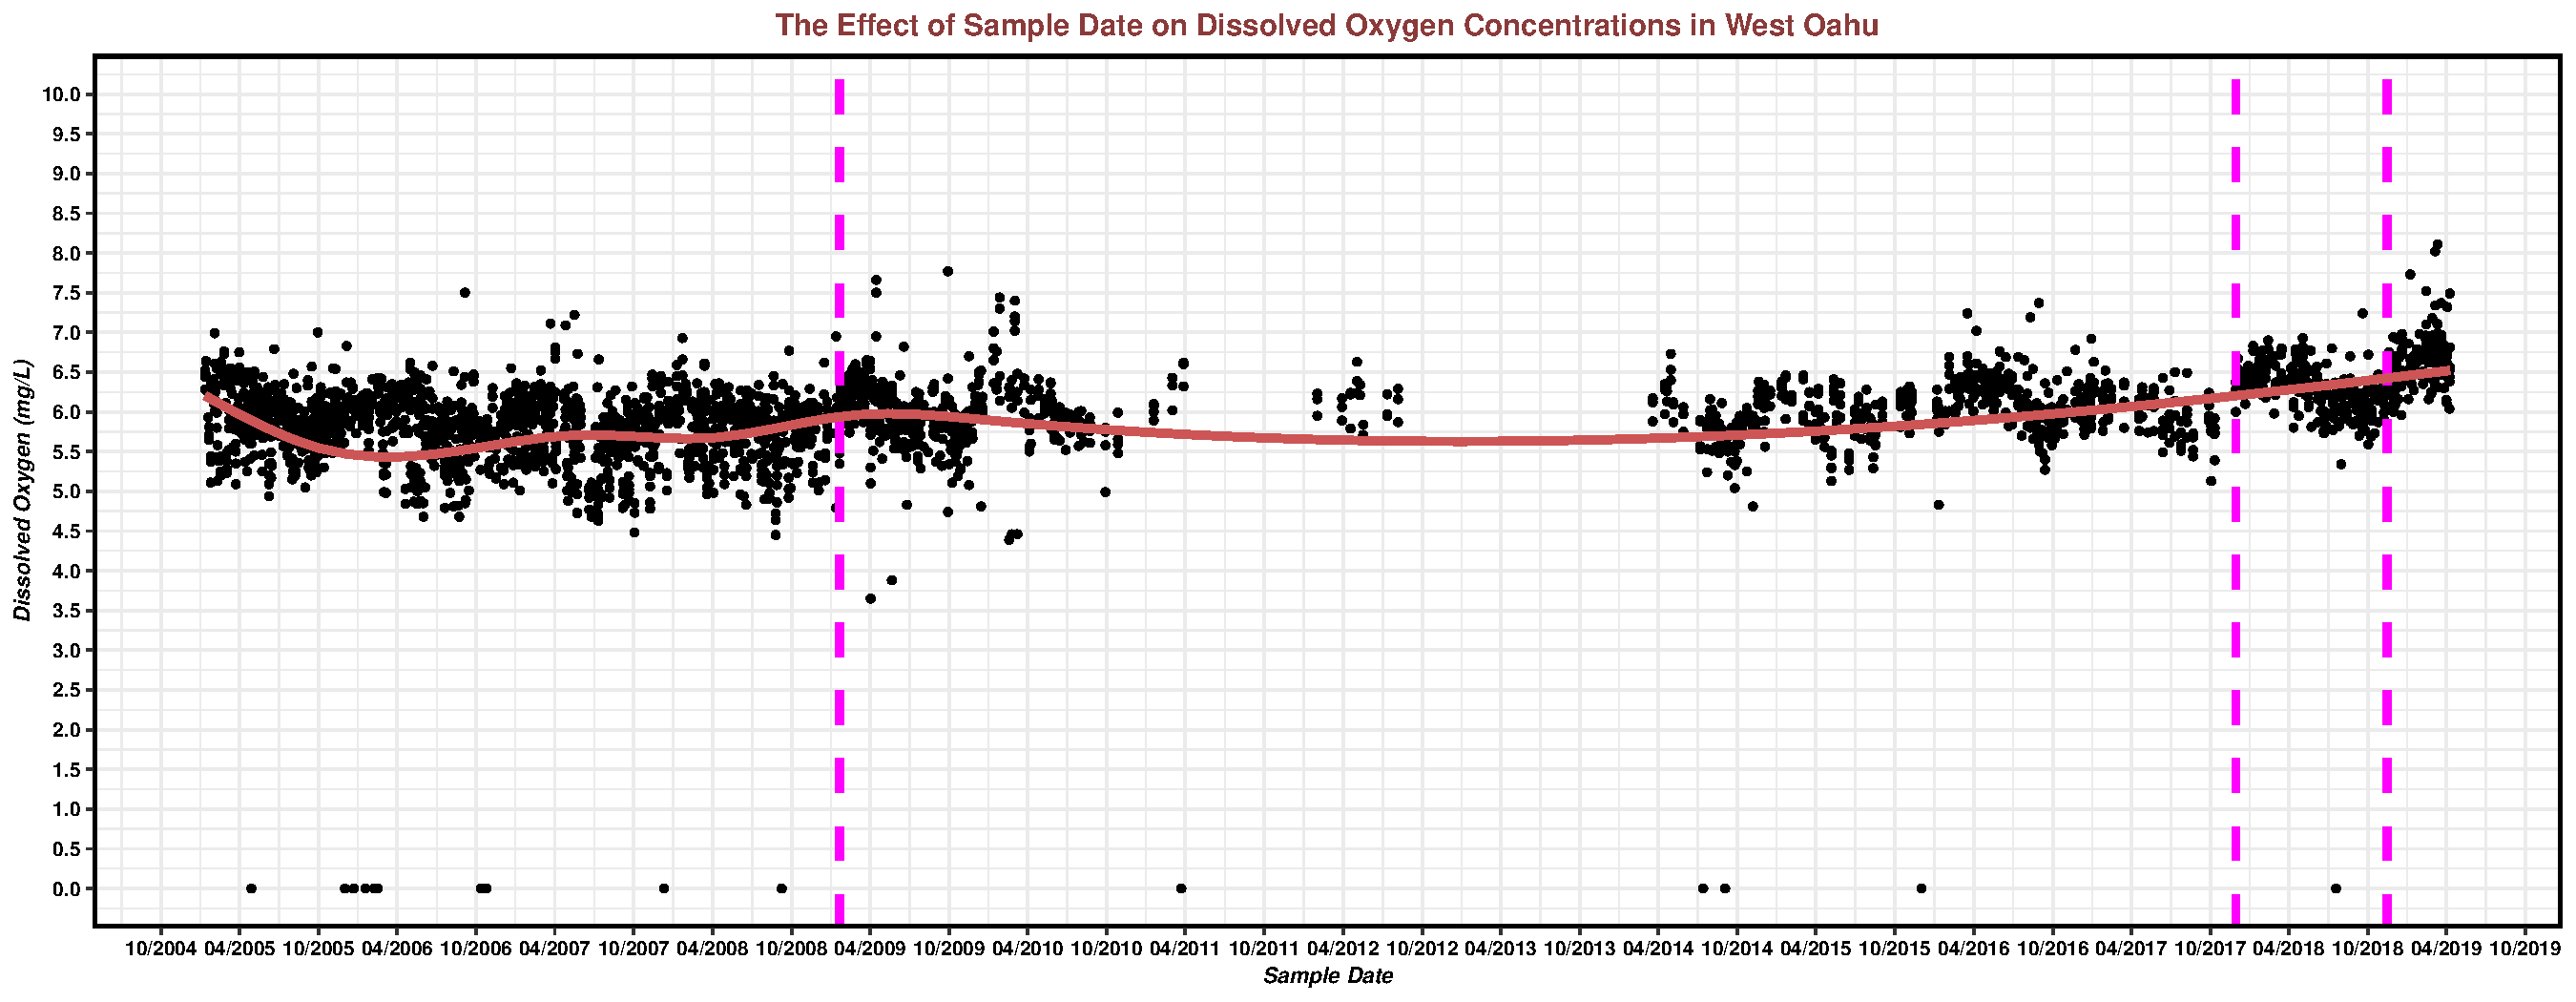
\includegraphics{Garcia_ENV872_Project_files/figure-latex/West Oahu-1.pdf}

\section{East Oahu}\label{east-oahu}

\subsubsection{Change Date to be a date
object}\label{change-date-to-be-a-date-object-3}

\begin{Shaded}
\begin{Highlighting}[]
\NormalTok{HawaiiWaterCleanOahuEast}\OperatorTok{$}\NormalTok{Date<-}\KeywordTok{as.Date}\NormalTok{(HawaiiWaterCleanOahuEast}\OperatorTok{$}\NormalTok{Date, }\DataTypeTok{format =} \StringTok{"%m/%d/%y"}\NormalTok{)}
\end{Highlighting}
\end{Shaded}

\subsubsection{Arrange East Oahu Dataset by Date
(ascending)}\label{arrange-east-oahu-dataset-by-date-ascending}

\begin{Shaded}
\begin{Highlighting}[]
\NormalTok{HawaiiWaterCleanOahuEast<-dplyr}\OperatorTok{::}\KeywordTok{arrange}\NormalTok{(HawaiiWaterCleanOahuEast, Date)}
\end{Highlighting}
\end{Shaded}

\subsection{Pettit's Test for East
Oahu}\label{pettits-test-for-east-oahu}

\begin{Shaded}
\begin{Highlighting}[]
\KeywordTok{pettitt.test}\NormalTok{(HawaiiWaterCleanOahuEast}\OperatorTok{$}\NormalTok{DO)}
\end{Highlighting}
\end{Shaded}

\begin{verbatim}
## 
##  Pettitt's test for single change-point detection
## 
## data:  HawaiiWaterCleanOahuEast$DO
## U* = 1848000, p-value < 2.2e-16
## alternative hypothesis: two.sided
## sample estimates:
## probable change point at time K 
##                            3549
\end{verbatim}

Because the p-value is \textless{}0.05, the change point is significant.
Given 1st change point for East Oahu is 3549, we scroll to observation
3549 in data set, so first change point occurred in 2014-11-17

\subsection{Run a separate Mann-Kendall Test for Each Change
Point}\label{run-a-separate-mann-kendall-test-for-each-change-point-3}

\begin{Shaded}
\begin{Highlighting}[]
\KeywordTok{mk.test}\NormalTok{(HawaiiWaterCleanOahuEast}\OperatorTok{$}\NormalTok{DO[}\DecValTok{1}\OperatorTok{:}\DecValTok{3548}\NormalTok{])}
\end{Highlighting}
\end{Shaded}

\begin{verbatim}
## 
##  Mann-Kendall trend test
## 
## data:  HawaiiWaterCleanOahuEast$DO[1:3548]
## z = -0.1326, n = 3548, p-value = 0.8945
## alternative hypothesis: true S is not equal to 0
## sample estimates:
##             S          varS           tau 
## -9.344000e+03  4.964278e+09 -1.490000e-03
\end{verbatim}

\begin{Shaded}
\begin{Highlighting}[]
\KeywordTok{mk.test}\NormalTok{(HawaiiWaterCleanOahuEast}\OperatorTok{$}\NormalTok{DO[}\DecValTok{3549}\OperatorTok{:}\DecValTok{4694}\NormalTok{])}
\end{Highlighting}
\end{Shaded}

\begin{verbatim}
## 
##  Mann-Kendall trend test
## 
## data:  HawaiiWaterCleanOahuEast$DO[3549:4694]
## z = 17.055, n = 1146, p-value < 2.2e-16
## alternative hypothesis: true S is not equal to 0
## sample estimates:
##            S         varS          tau 
## 2.206860e+05 1.674337e+08 3.375283e-01
\end{verbatim}

p-value for {[}3549:4694{]} is significant, so run a Pettit's Test

\subsection{What is second change
point?}\label{what-is-second-change-point-2}

\begin{Shaded}
\begin{Highlighting}[]
\KeywordTok{pettitt.test}\NormalTok{(HawaiiWaterCleanOahuEast}\OperatorTok{$}\NormalTok{DO[}\DecValTok{3549}\OperatorTok{:}\DecValTok{4694}\NormalTok{])}
\end{Highlighting}
\end{Shaded}

\begin{verbatim}
## 
##  Pettitt's test for single change-point detection
## 
## data:  HawaiiWaterCleanOahuEast$DO[3549:4694]
## U* = 198770, p-value < 2.2e-16
## alternative hypothesis: two.sided
## sample estimates:
## probable change point at time K 
##                             614
\end{verbatim}

3549+ 614=4163, so look at 4163th row-\textgreater{} second change point
occurred on 2017-11-27

\section{Run another Mann-Kendall for the third change
point}\label{run-another-mann-kendall-for-the-third-change-point}

\paragraph{Now split dataset into three
pieces}\label{now-split-dataset-into-three-pieces-3}

\begin{Shaded}
\begin{Highlighting}[]
\KeywordTok{mk.test}\NormalTok{(HawaiiWaterCleanOahuEast}\OperatorTok{$}\NormalTok{DO[}\DecValTok{3549}\OperatorTok{:}\DecValTok{4162}\NormalTok{])   }
\end{Highlighting}
\end{Shaded}

\begin{verbatim}
## 
##  Mann-Kendall trend test
## 
## data:  HawaiiWaterCleanOahuEast$DO[3549:4162]
## z = 0.56625, n = 614, p-value = 0.5712
## alternative hypothesis: true S is not equal to 0
## sample estimates:
##            S         varS          tau 
## 2.876000e+03 2.577866e+07 1.534538e-02
\end{verbatim}

\begin{Shaded}
\begin{Highlighting}[]
\KeywordTok{mk.test}\NormalTok{(HawaiiWaterCleanOahuEast}\OperatorTok{$}\NormalTok{DO[}\DecValTok{4163}\OperatorTok{:}\DecValTok{4694}\NormalTok{])  }
\end{Highlighting}
\end{Shaded}

\begin{verbatim}
## 
##  Mann-Kendall trend test
## 
## data:  HawaiiWaterCleanOahuEast$DO[4163:4694]
## z = 4.6476, n = 532, p-value = 3.359e-06
## alternative hypothesis: true S is not equal to 0
## sample estimates:
##            S         varS          tau 
## 1.903600e+04 1.677464e+07 1.353027e-01
\end{verbatim}

Because p\textless{}0.05, there is a significant change point in rows
{[}4163:4694{]}

\subsection{Third Change Point}\label{third-change-point-2}

\begin{Shaded}
\begin{Highlighting}[]
\KeywordTok{pettitt.test}\NormalTok{(HawaiiWaterCleanOahuEast}\OperatorTok{$}\NormalTok{DO[}\DecValTok{4163}\OperatorTok{:}\DecValTok{4694}\NormalTok{])}
\end{Highlighting}
\end{Shaded}

\begin{verbatim}
## 
##  Pettitt's test for single change-point detection
## 
## data:  HawaiiWaterCleanOahuEast$DO[4163:4694]
## U* = 34049, p-value < 2.2e-16
## alternative hypothesis: two.sided
## sample estimates:
## probable change point at time K 
##                             351
\end{verbatim}

Third change point is 4163+ 351=4514, which happened on 2018-12-04

\section{Time Series of DO Concentrations in East Oahu with
Changepoints}\label{time-series-of-do-concentrations-in-east-oahu-with-changepoints}

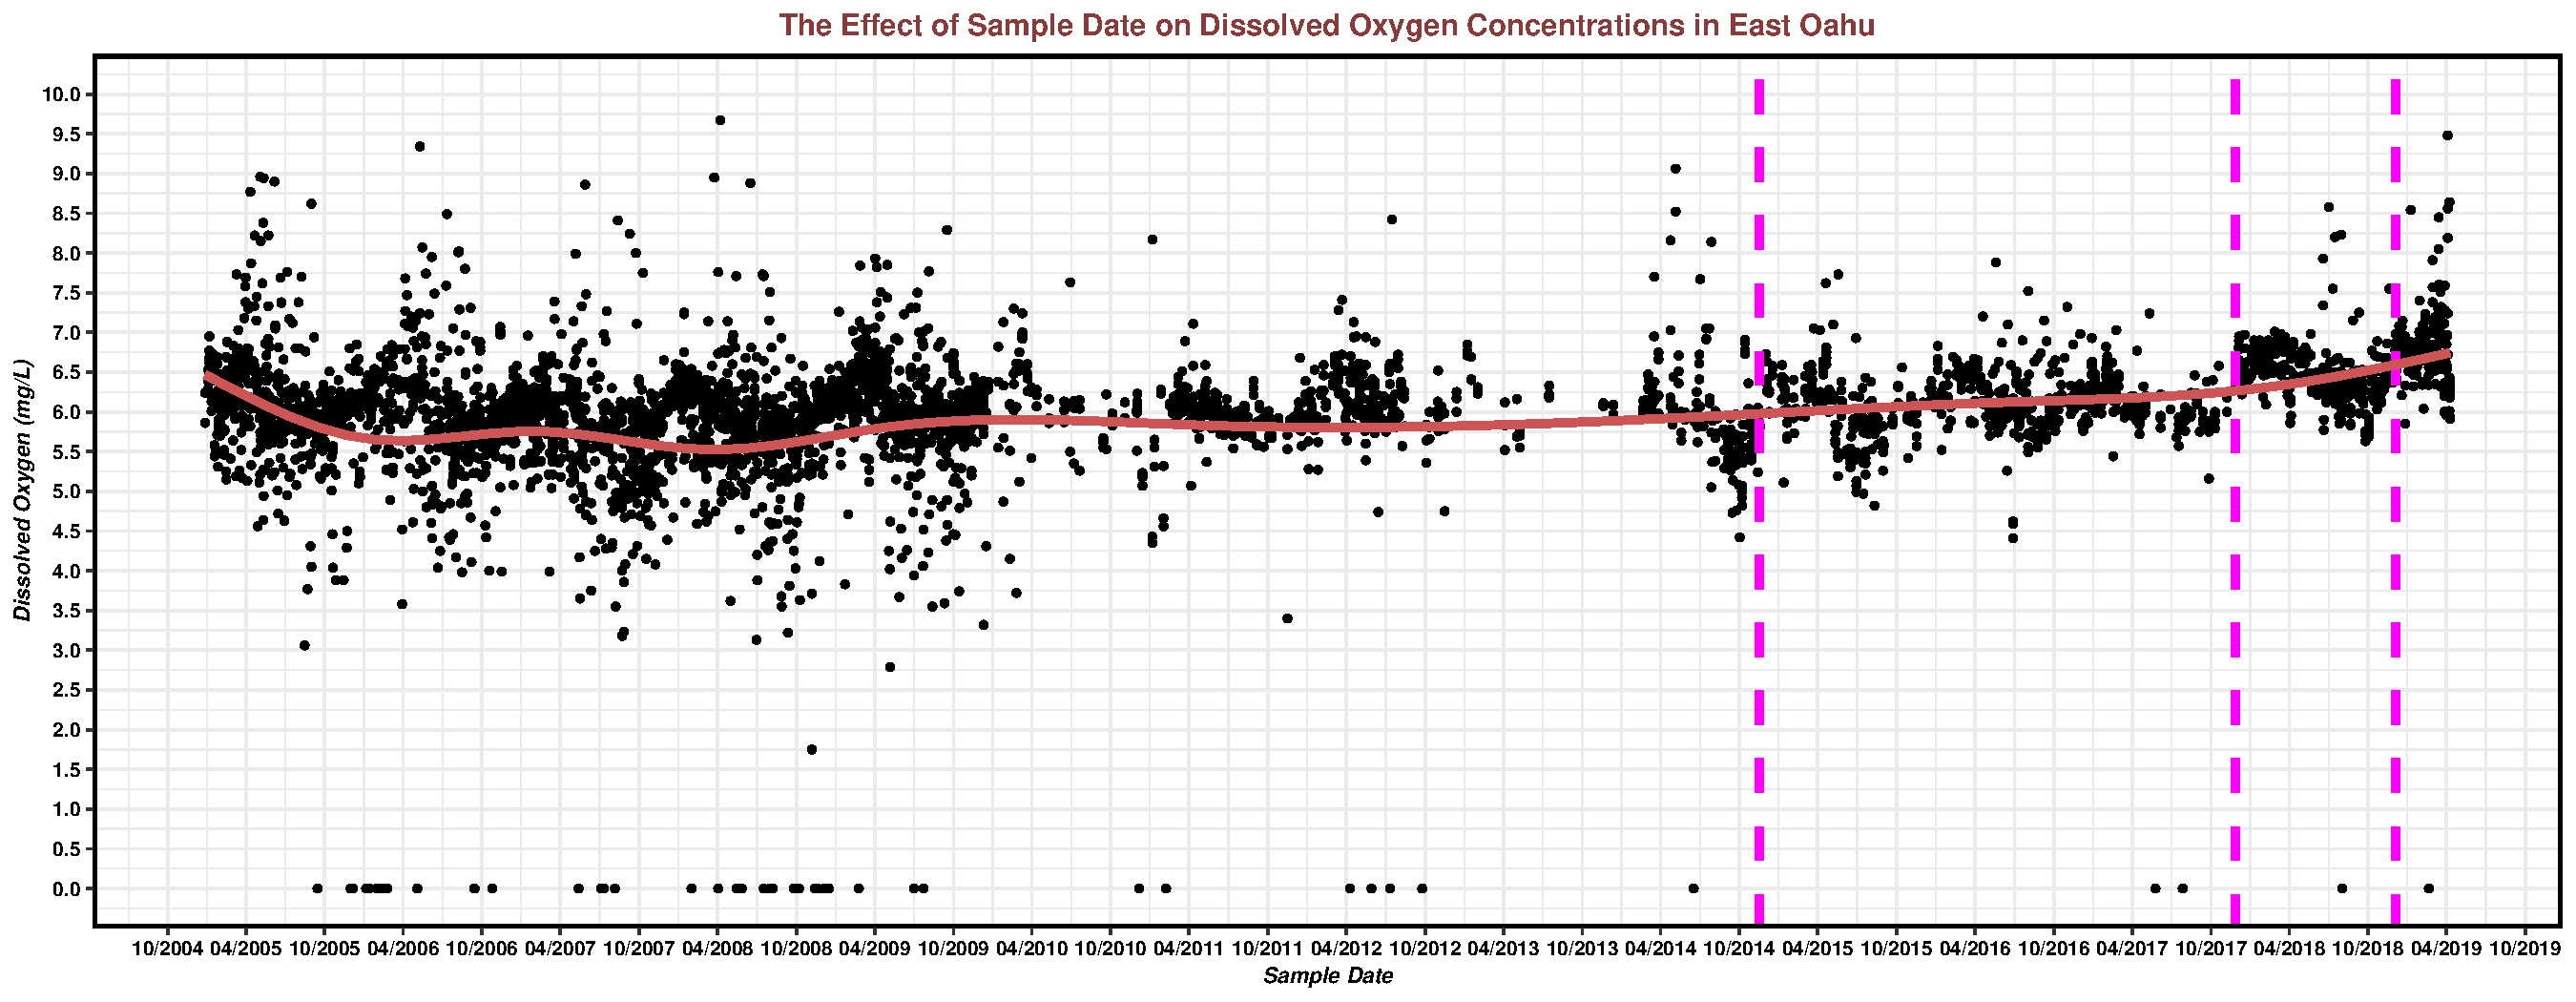
\includegraphics{Garcia_ENV872_Project_files/figure-latex/East Oahu-1.pdf}

\section{Effect of Sample Date on Dissolved Oxygen
Concentration}\label{effect-of-sample-date-on-dissolved-oxygen-concentration}

\subsubsection{Change Date to Date
Object}\label{change-date-to-date-object}

\begin{Shaded}
\begin{Highlighting}[]
\NormalTok{OahuDataClean}\OperatorTok{$}\NormalTok{Date<-}\KeywordTok{as.Date}\NormalTok{(OahuDataClean}\OperatorTok{$}\NormalTok{Date,}\DataTypeTok{format =} \StringTok{"%m/%d/%y"}\NormalTok{)}
\end{Highlighting}
\end{Shaded}

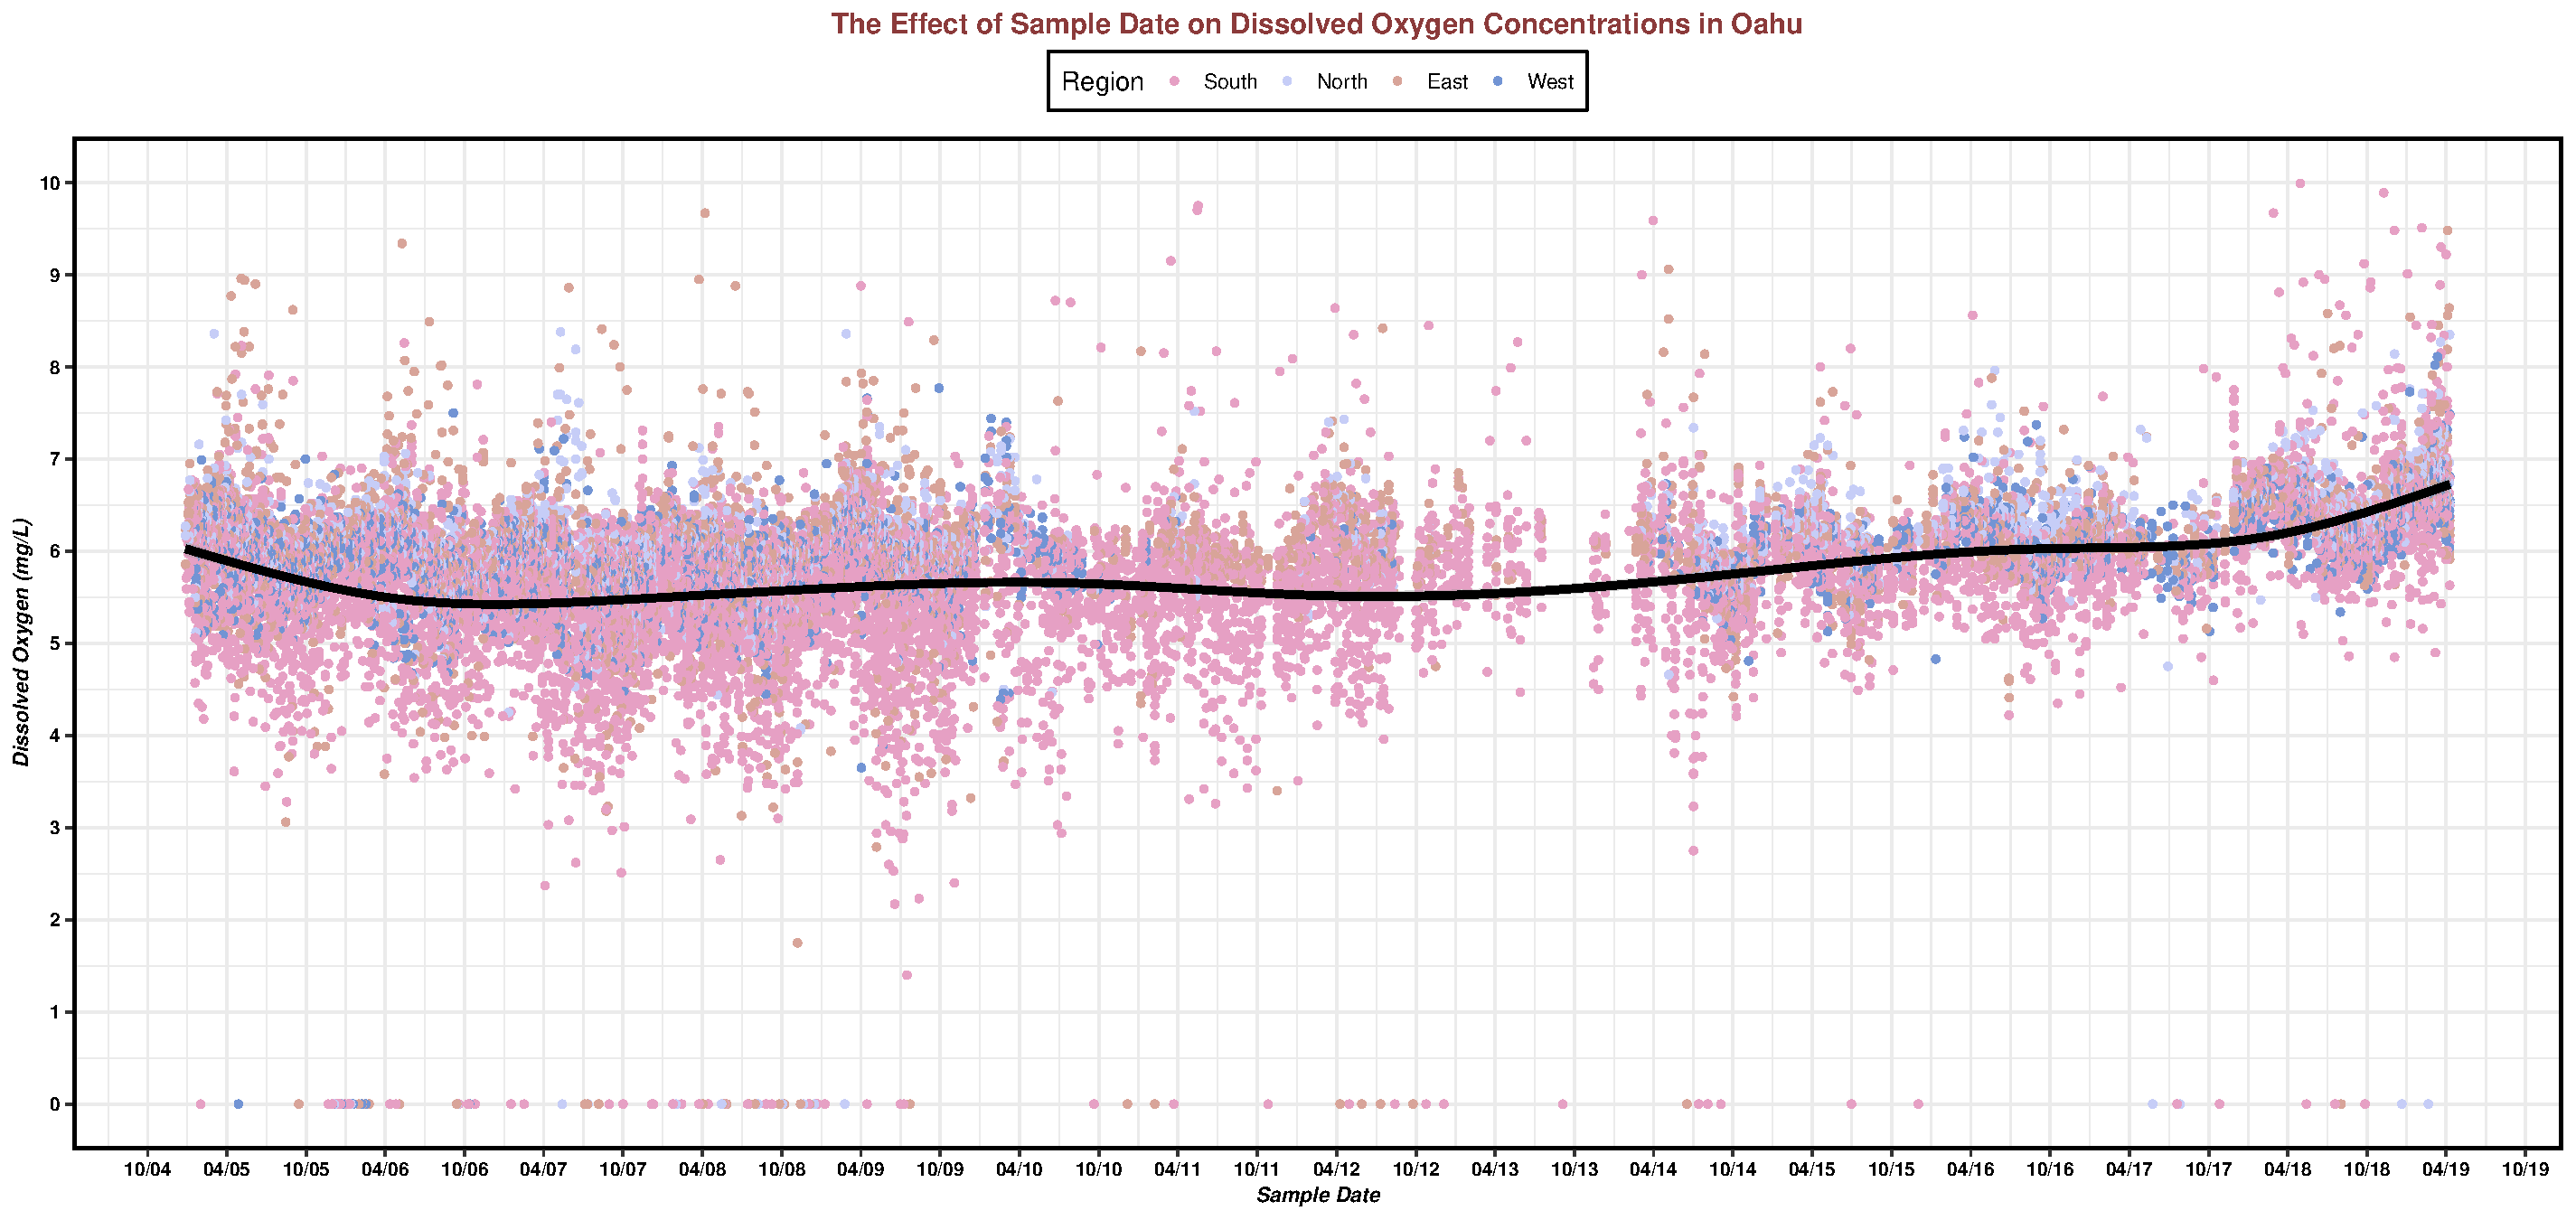
\includegraphics{Garcia_ENV872_Project_files/figure-latex/DO-1.pdf}

\section{Effect of Sample Date on Water Temperature in
Oahu}\label{effect-of-sample-date-on-water-temperature-in-oahu}

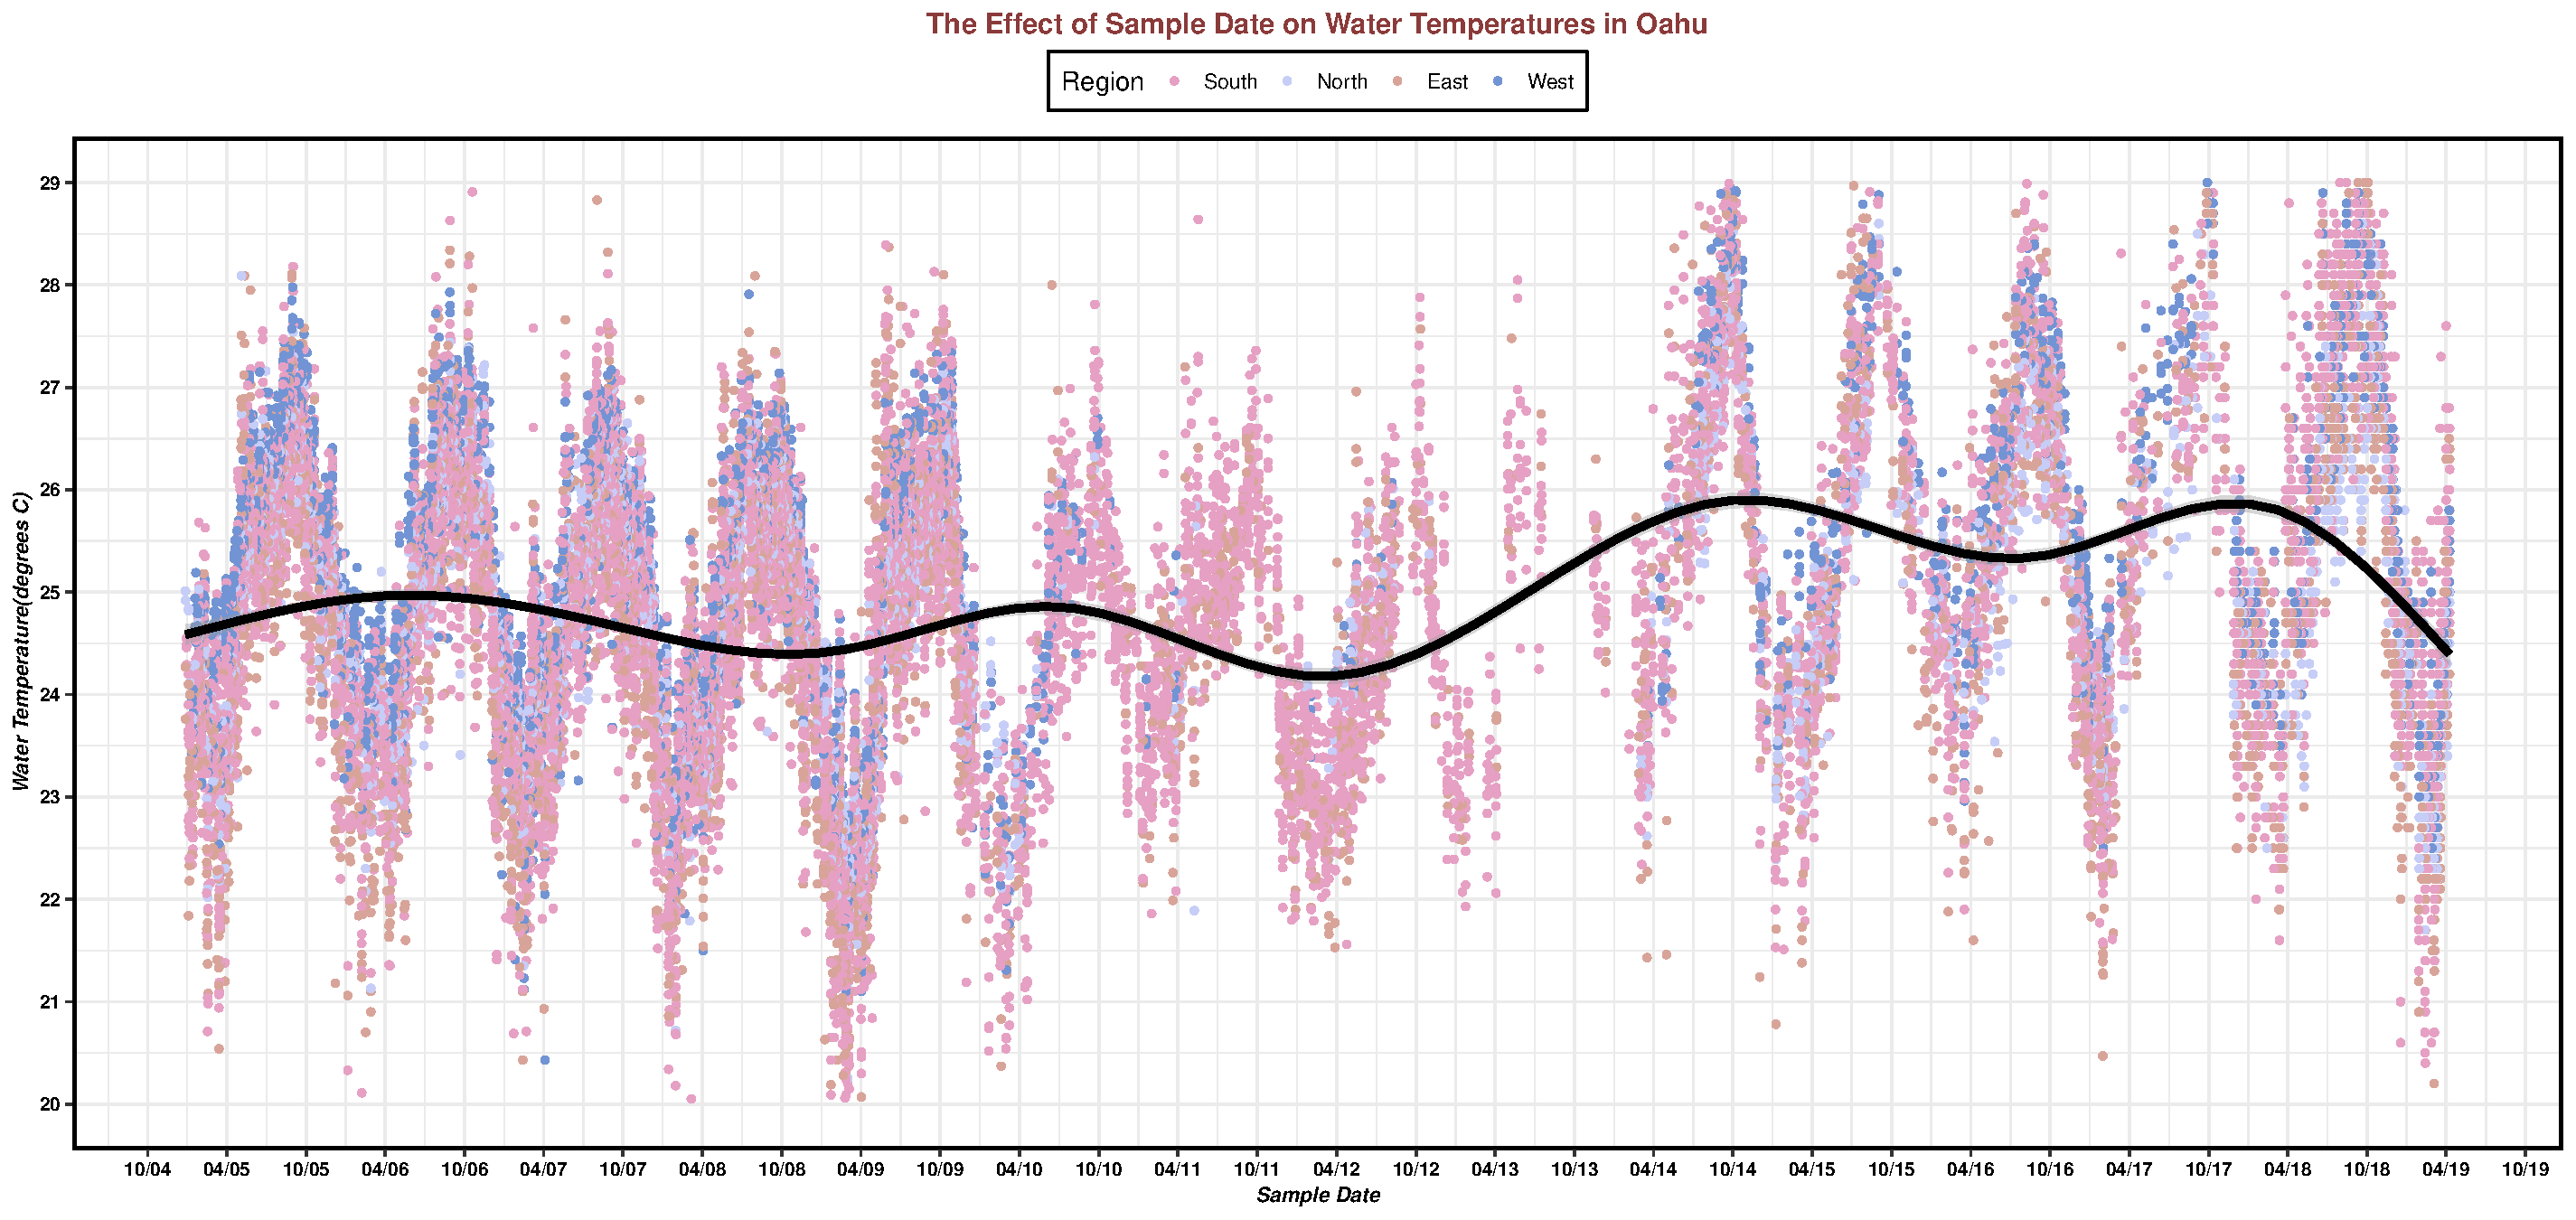
\includegraphics{Garcia_ENV872_Project_files/figure-latex/Temp-1.pdf}

\section{Effect of Sample Date on pH in
Oahu}\label{effect-of-sample-date-on-ph-in-oahu}

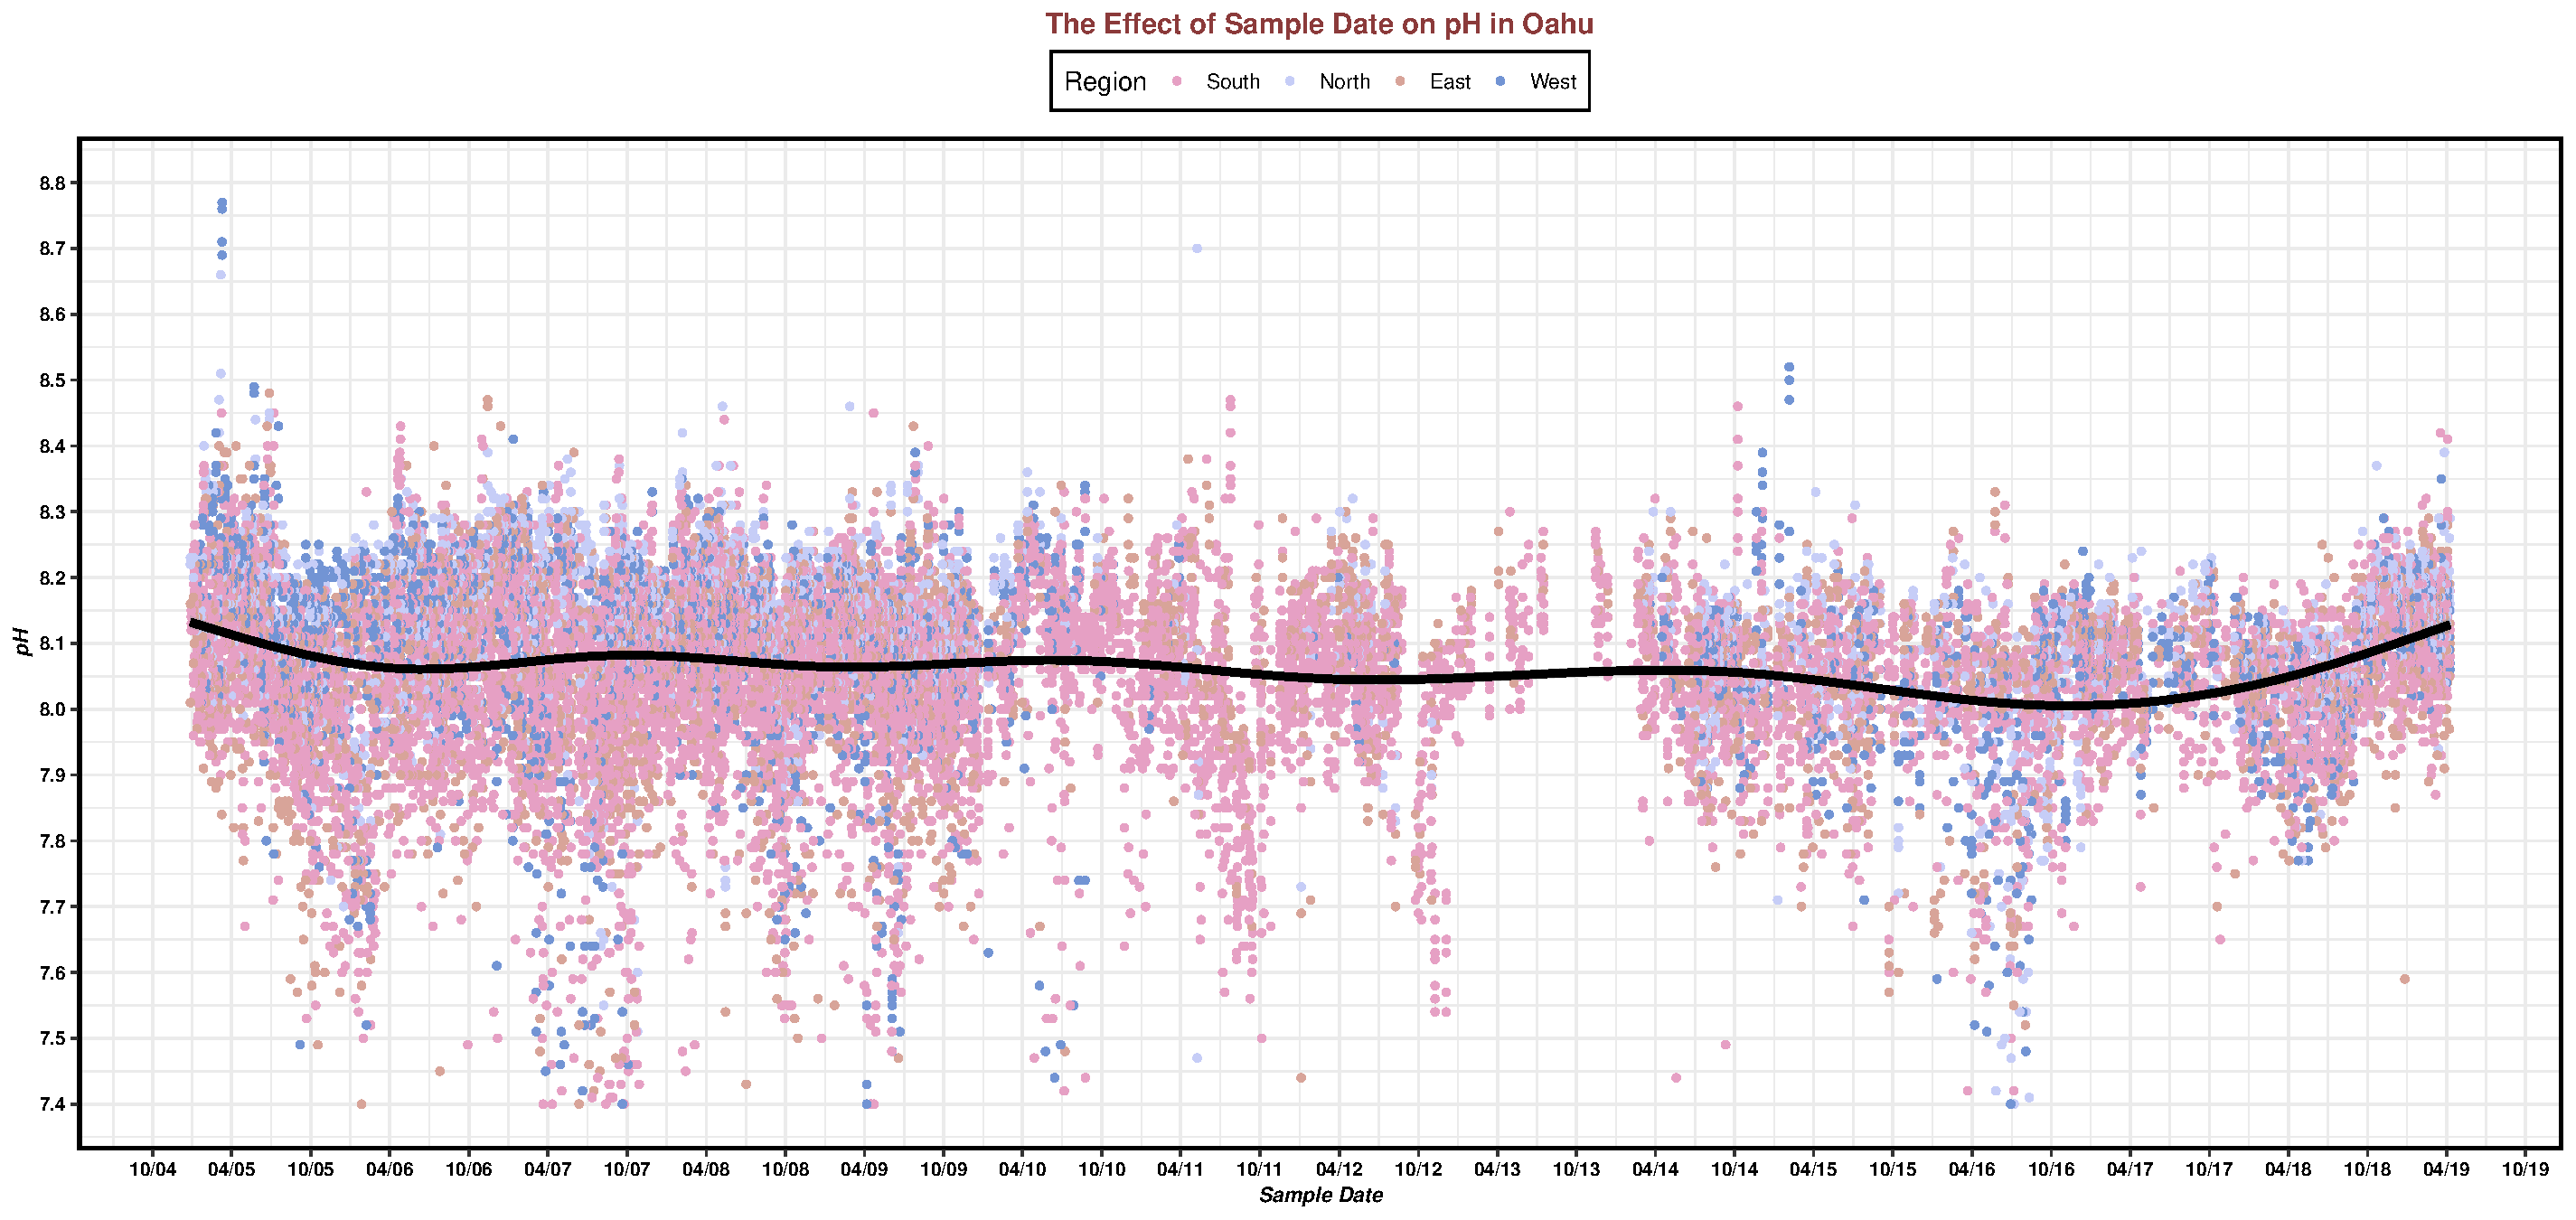
\includegraphics{Garcia_ENV872_Project_files/figure-latex/pH-1.pdf}

\section{Effect of Sample Date on Salinity in
Oahu}\label{effect-of-sample-date-on-salinity-in-oahu}

\begin{Shaded}
\begin{Highlighting}[]
\KeywordTok{library}\NormalTok{(wesanderson)}
\NormalTok{OahuSalinityPlot<-}\KeywordTok{ggplot}\NormalTok{(OahuDataClean, }\KeywordTok{aes}\NormalTok{(}\DataTypeTok{x =}\NormalTok{ Date, }\DataTypeTok{y =}\NormalTok{Salinity, }\DataTypeTok{color =}\NormalTok{ Region)) }\OperatorTok{+}\StringTok{ }
\StringTok{  }\KeywordTok{geom_point}\NormalTok{(}\DataTypeTok{alpha=}\DecValTok{1}\NormalTok{) }\OperatorTok{+}
\KeywordTok{scale_color_manual}\NormalTok{(}\DataTypeTok{values=}\KeywordTok{wes_palette}\NormalTok{(}\DataTypeTok{name=}\StringTok{"GrandBudapest2"}\NormalTok{)) }\OperatorTok{+}
\StringTok{  }\NormalTok{##geom_vline(xintercept=as.Date("2004-08-16"),color="253494", origin= "1970-01-01", lty=2) + ###First Change Point for North Oahu }
\StringTok{ }\NormalTok{## geom_vline(xintercept=as.Date("2005-08-17"), color="253494", origin= "1970-01-01", lty=2)  ###Second Change Point for North Oahu }

\StringTok{  }\KeywordTok{geom_smooth}\NormalTok{(}\KeywordTok{aes}\NormalTok{(}\DataTypeTok{x =}\NormalTok{ Date, }\DataTypeTok{y =}\NormalTok{Salinity, }\DataTypeTok{span=}\FloatTok{0.1}\NormalTok{), }\DataTypeTok{color=}\StringTok{"black"}\NormalTok{, }\DataTypeTok{linetype=}\DecValTok{1}\NormalTok{, }\DataTypeTok{size=}\DecValTok{2}\NormalTok{) }\OperatorTok{+}
\StringTok{  }\KeywordTok{labs}\NormalTok{(}\DataTypeTok{title=}\StringTok{"The Effect of Sample Date on Salinity in Oahu"}\NormalTok{, }
       \DataTypeTok{x=}\StringTok{"Sample Date"}\NormalTok{,}
       \DataTypeTok{y=}\StringTok{"Salinity (ppt)"}\NormalTok{) }\OperatorTok{+}

\StringTok{ }\KeywordTok{scale_x_date}\NormalTok{(}\DataTypeTok{labels =} \KeywordTok{date_format}\NormalTok{(}\StringTok{"%m/%y"}\NormalTok{), }\DataTypeTok{breaks =} \KeywordTok{date_breaks}\NormalTok{(}\StringTok{"6 month"}\NormalTok{)) }\OperatorTok{+}
\KeywordTok{scale_y_continuous}\NormalTok{(}\DataTypeTok{limits=}\KeywordTok{c}\NormalTok{(}\DecValTok{0}\NormalTok{,}\DecValTok{40}\NormalTok{), }\DataTypeTok{breaks=}\KeywordTok{seq}\NormalTok{(}\DecValTok{0}\NormalTok{, }\DecValTok{40}\NormalTok{, }\DataTypeTok{by =} \DecValTok{5}\NormalTok{))}


\NormalTok{OahuSalinityPlot}
\end{Highlighting}
\end{Shaded}

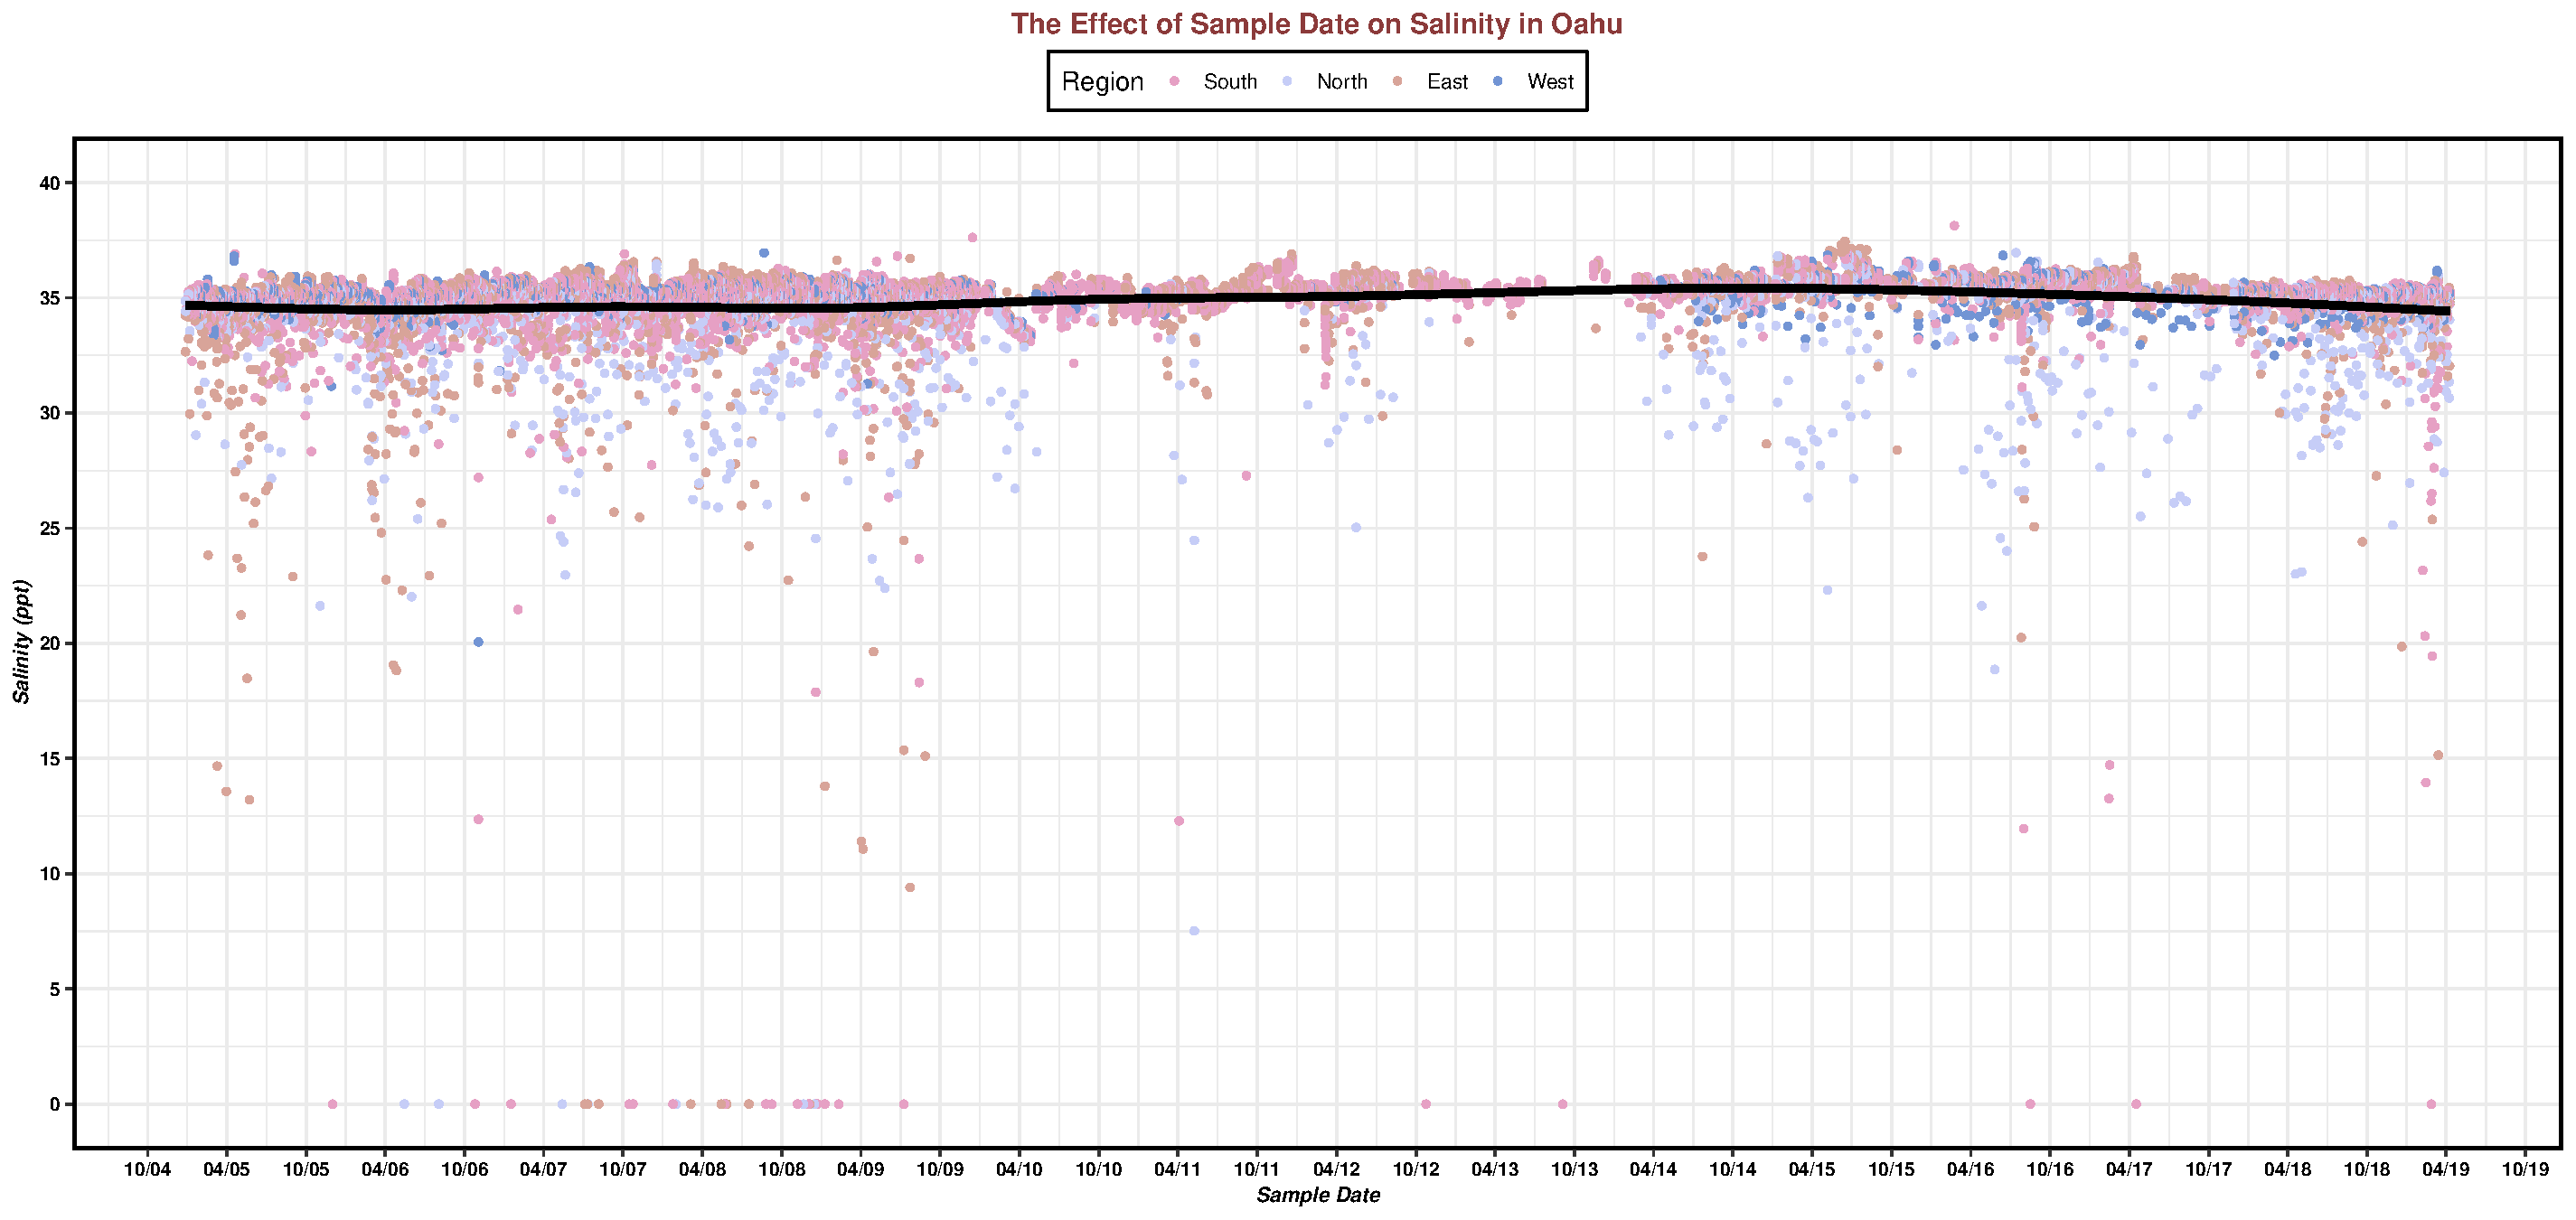
\includegraphics{Garcia_ENV872_Project_files/figure-latex/Salinity-1.pdf}

\section{Comparison of pH, DO and Temperature over Time in
Oahu}\label{comparison-of-ph-do-and-temperature-over-time-in-oahu}

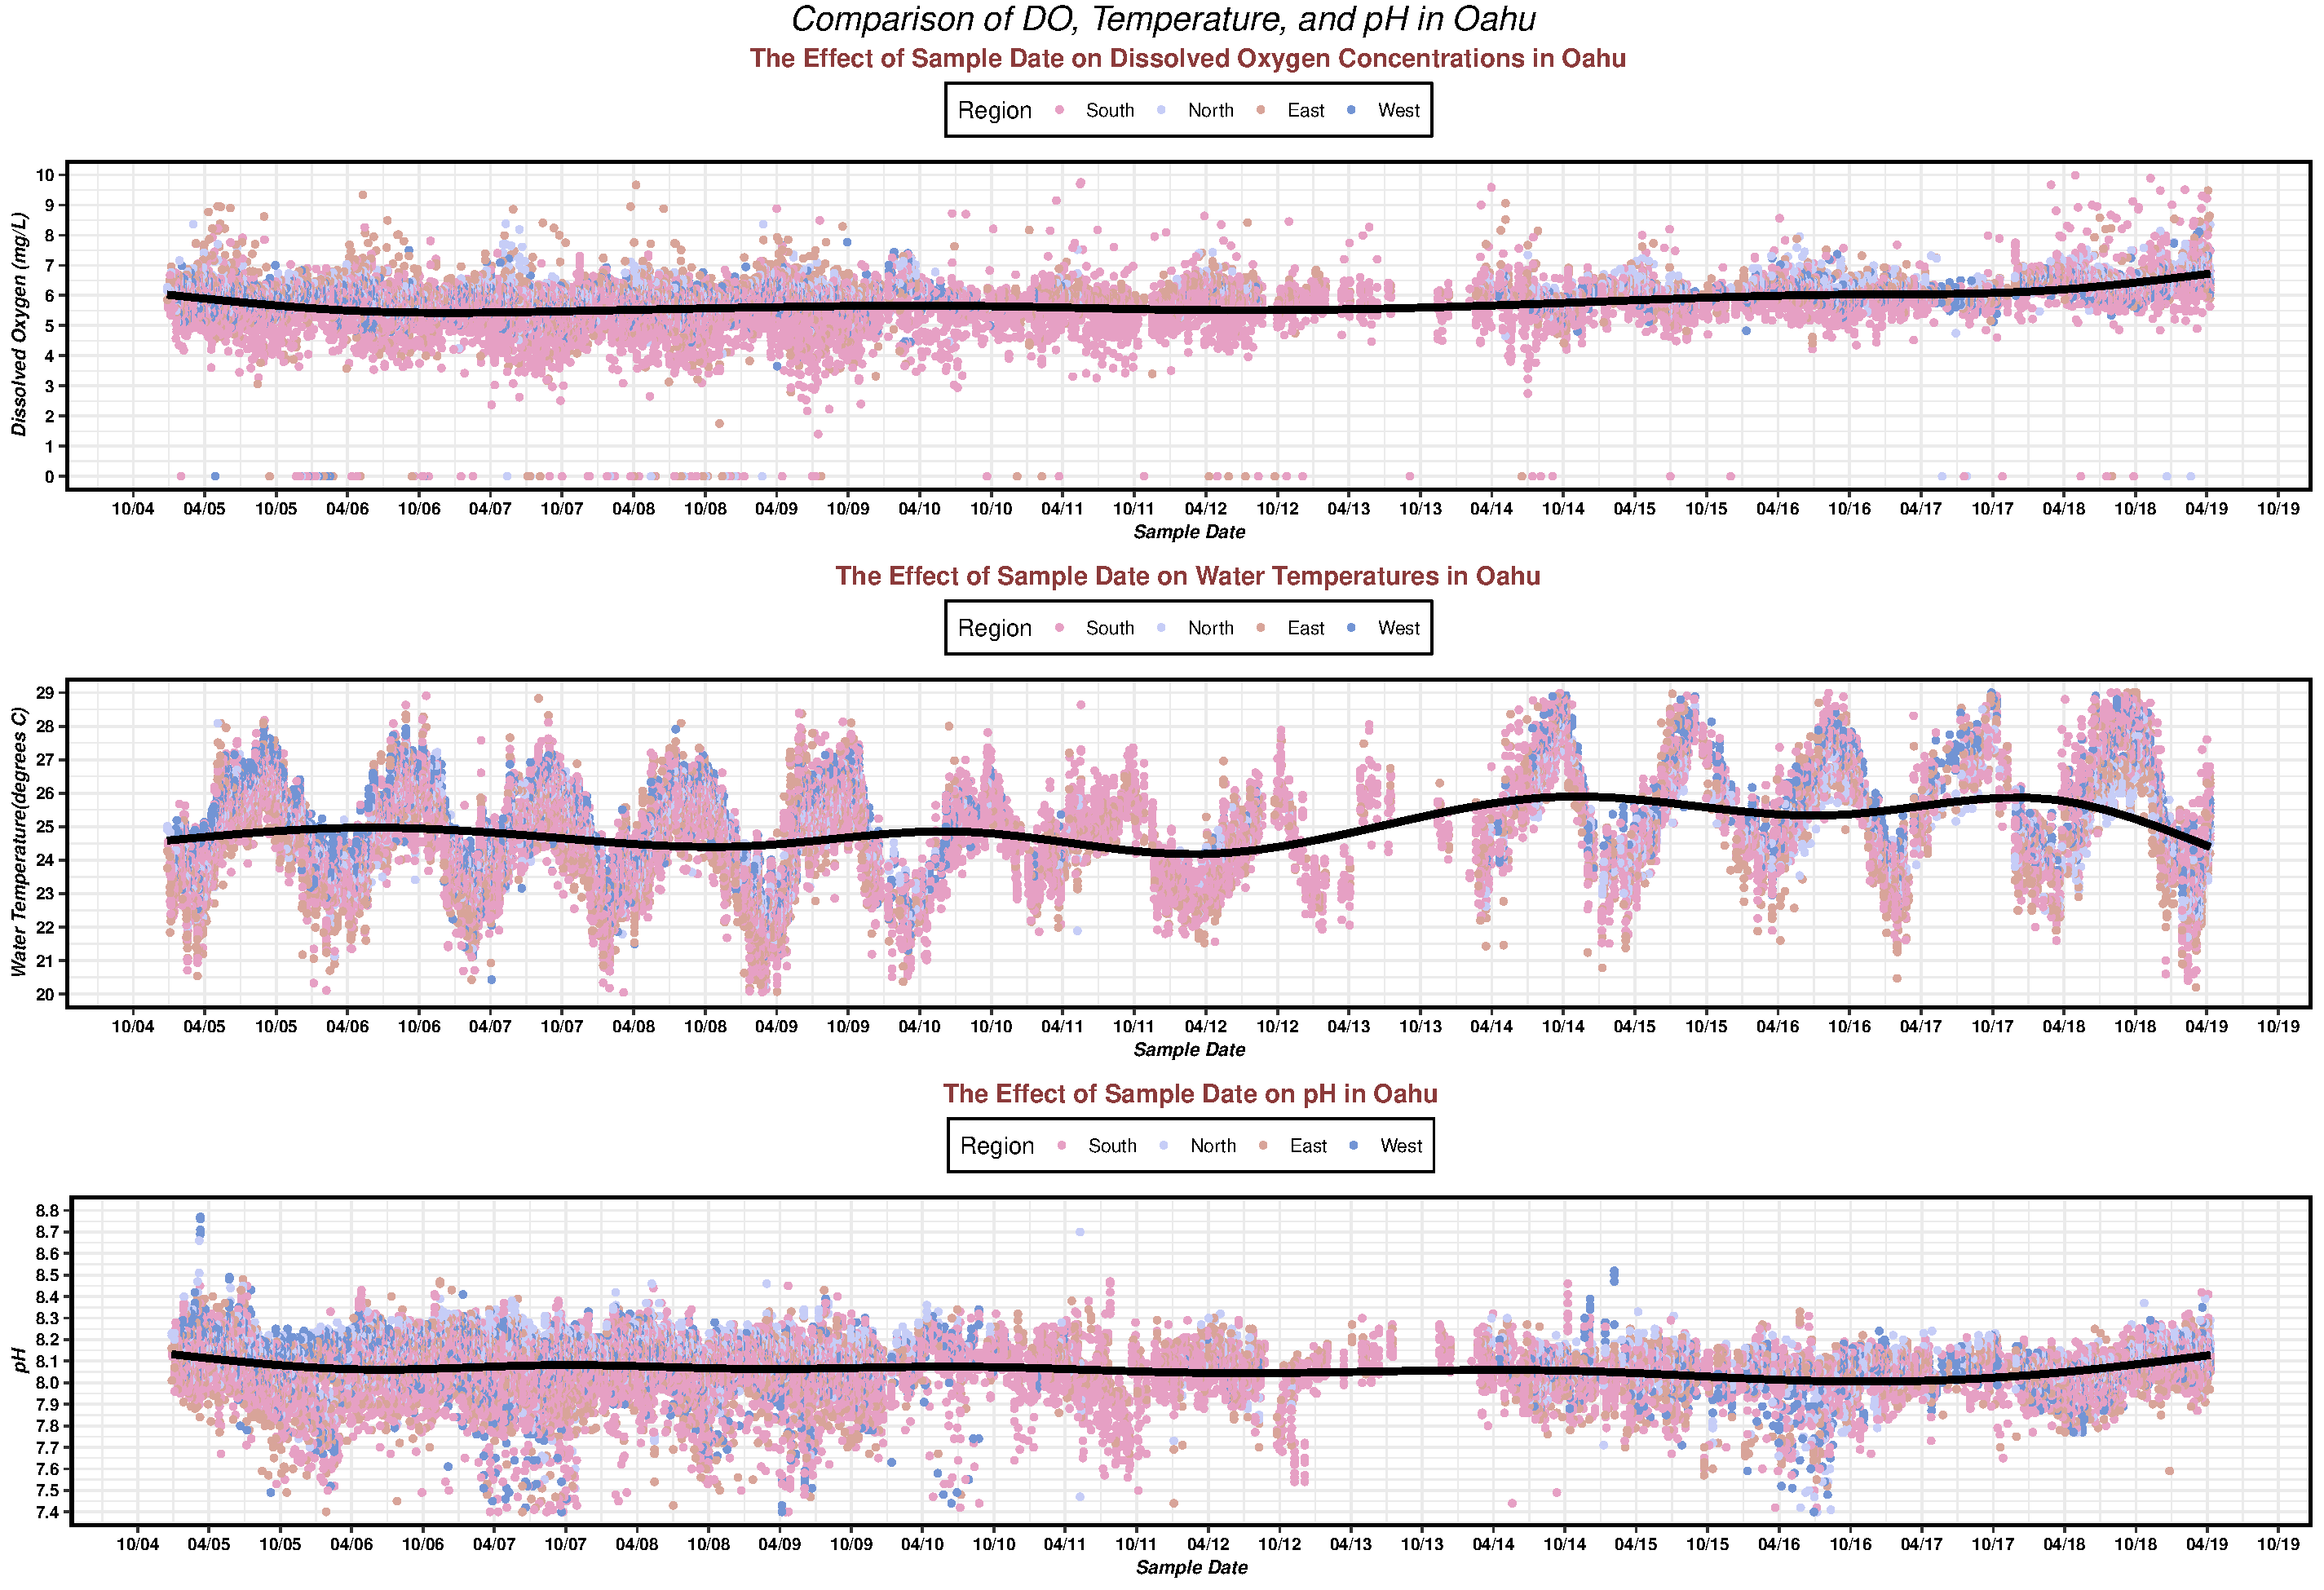
\includegraphics{Garcia_ENV872_Project_files/figure-latex/unnamed-chunk-98-1.pdf}

\section{Spatial Analysis}\label{spatial-analysis}

\subsection{Compute Mean DO, Mean Temp, and Mean Salinity by Oahu Sample
Location}\label{compute-mean-do-mean-temp-and-mean-salinity-by-oahu-sample-location}

\begin{Shaded}
\begin{Highlighting}[]
\NormalTok{OahuDataCleanAvg<-OahuDataClean}\OperatorTok\StringTok{ }
\StringTok{   }\KeywordTok{group_by}\NormalTok{(LocationName, LocationIdentifier, Region, LatDecDeg, LongDecDeg) }\OperatorTok\StringTok{ }
\StringTok{  }\KeywordTok{summarize}\NormalTok{(}\DataTypeTok{meanDO=} \KeywordTok{mean}\NormalTok{(DO),}
            \DataTypeTok{meanTemp =} \KeywordTok{mean}\NormalTok{(Temperature),}
            \DataTypeTok{meanTurbidity=}\KeywordTok{mean}\NormalTok{(Turbidity)) }
\end{Highlighting}
\end{Shaded}

\section{Summary and Conclusions}\label{summary-and-conclusions-1}

Using exploratory plots, I found that the data is not normally
distributed, like most environmental datasets. As seen by my exploratory
plots, some of my variables were right skewed with some extreme values
and outliers. However, assumptions of multiple linear regression are
independence of error terms, homoscedasticity(constant variance) of
errors, normality of the error distribution, explanatory variables are
fixed, and no perfect multicollinearity. I decided to proceed with a
multiple linear regression, as my residual errors looked fine. The
maximal model is HawaiiModClean with all relevant independent variables
included. Using my GGPairs Bivariate scatterplots for all variable
combinations allowed me to look at the correlation coefficients between
each variable combination, to ensure there is no multicollinearity
between the independent variables, and the independent and dependent
variables are linearly correlated. Enterococcus and DO have almost no
correlation: 0.005. Temperature and DO have a low positive correlation:
0.104. Salinity and DO have a low positive correlation: 0.147. pH and DO
have a low positive correlation: 0.169. Turbidity and DO have almost no
correlation: -0.019. Percent Saturation DO and DO are multicollineated
because they are related variables, so I did not include Percent
Saturation of DO in my analysis.

I used the stepwise reduction methodto remove the least significant
independent variables from the maximal model until only the independent
variables with a significant effect on dissolved oxygen concentrations
were left, leaving the most parsimonious model HawaiiModClean3. An AIC
test was done comparing our final reduced model to our fuller models to
determine a goodness of fit score. Our final reduced model had an AIC
score 77790.15. While this wasn't the lowest model score, it was within
three points of the next score, and Turbidity was not statistically
significant with a p-value \textgreater{}0.05, so I removed it. My
multiple linear regression found that the explanatory parameters of
temperature, pH, salinity, and Enterococci concentrations were
significant predictors of dissolved oxygen concentrations in Oahu. A VIF
test found that none of these parameters suffered from
multicollinearity. The following are their respective statistics:
Temperature (p=4.34e-05, t=4.09), Enterococcus (t=2.42, p=0.015),
Salinity (t=13.096, p\textless{}2e-16), and pH(t=19.03,
p\textless{}2e-16). Based on the model coefficients, a one degree
Celsius increase in temperature will result in an increase in dissolved
oxygen concentrations by 0.02 mg/L. A one ppt increase in Salinity will
result in an increase in dissolved oxygen concentrations by 0.042 mg/L.
A one unit increase in pH will result in an increase in dissolved oxygen
concentrations by 0.17 mg/L. A one unit increase in Enterococcus will
result in an increase in dissolved oyxgen concentrations by 9.99e-5
mg/L. (Linear Regression; p\textless{}0.05, df=15,449, Rsqaured=0.04).
The linear equation for my regression is Dissolved Oxygen=2.42 +
0.02(Temperature)+0.042(Salinity) + 0.17(pH) +9.99e-5(Enterococcus) + E.
If I had more time, I would have researched interactions between these
parameters to see which interactions would have been the most beneficial
to include in my maximal model. My model only explains 4\% of the
variability of the data around its mean, and perhaps certain
interactions would account for more of the variability.

If I had more available parameters in my data such as phosphorus and
nitrate concentrations, they might explain more of the variability in my
dataset that my multiple linear regression failed to explain. Phoshorus
and nitrate often end up in water bodies as runoff from
agriculture/anthropogenic activity and deplete the dissolved oxygen
necessary for aerobic activity in water bodies. Because Honolulu (the
capital of Hawaii) is on the South coast of Oahu, I surmise that DO
concentrations would be lower on the south coast if I was able to
include phosphorus and nitrate measurements in my data. In addition, if
I had data on marine organisms (that use up oxygen) or ocean
circulation/stratification, that would also explain more of the
variability.

My second research question concerned whether dissolved oxygen
concentrations varied spatially across the North, South, East, and West
coasts of Oahu. An exploratory boxplot showed that the median of DO
concentrations on the South Coast was slightly lower than the median DO
Concentrations of the North, West, and East coasts. Honolulu is located
on the South coast and several samples were taken by the capital city,
but this is not enough evidence to draw a conclusion.


\end{document}
